% =============================================================================
% APPENDIX IE: CORE-EIT: Emergent Intervention Theory
% =============================================================================
% Module: BCM2_13_INT9250 (Interventionsbaukasten - Theoretical Foundation)
% Category: CORE
% Version: 3.8 (January 2026) - Added Intervention Specification Schema (EIT-EMP-3-D4)
%          v3.7: Added Scope-Mechanism Affinity Matrix (EIT-EMP-3-D2-EXT)
%          v3.6: Added Scope Level Emergence (EIT-EMP-3), Theorem EIT-T16
%          v3.5: Added EMERGE Algorithm (EIT-EMP-2), Extended Gamma Emergence
%          v3.4: Added γ_ij Complementarity Matrix (EIT-EMP-1)
%          v3.3: Added Central Question (Grundfrage) section
%          v3.2: Added 10 TODOs (TODO-IE-1 to TODO-IE-10) for Chapter 17-20 support
%          v3.1: Added explicit axiom type annotations (structural/empirical/theoretical)
%          per SSOT epistemology definition. Full axiom system (15 axioms), theorem system (12 theorems),
%          Critical Foundations, Open Issues sections for SSOT compliance
% Status: Final
% Language: English
%
% PURPOSE: This appendix formalizes the Emergent Intervention Theory (EIT),
% providing the theoretical foundation for intervention design. It establishes
% that interventions exist in a continuous 9-dimensional space, with "types"
% as emergent clusters rather than ontological primitives.
%
% SEPARATION OF CONCERNS:
% - IE (this appendix): Foundational theory (Axioms, Emergence Modes, Data Requirements)
% - HHH (METHOD-TOOLKIT): Operational tools (20-Field Schema, A1-A8, LLMMC protocols)
%
% =============================================================================

% -----------------------------------------------------------------------------
% HEADER BLOCK (Required)
% -----------------------------------------------------------------------------

\begin{tcolorbox}[colback=gray!5!white, colframe=gray!75!black,
    title=Appendix Header: IE CORE-EIT]

\begin{tabular}{@{}ll@{}}
\textbf{Code:} & IE \\
\textbf{Category:} & CORE (Fundamental Theory) \\
\textbf{Full Name:} & CORE-EIT: Emergent Intervention Theory \\
\textbf{Module:} & BCM2\_13\_INT9250 (Interventionsbaukasten) \\
\textbf{Version:} & 3.8 (January 2026) \\
\textbf{Status:} & Final \\
\textbf{Language:} & English \\
\end{tabular}

\vspace{0.5em}
\textbf{Purpose:} Formalizes the \textbf{Emergent Intervention Theory (EIT)}:
The theoretical foundation showing that interventions exist in a continuous
9-dimensional space $[0,1]^9$, with heuristic clusters (A1--A8) as emergent
clusters. Defines emergence modes (E-Full, E-Partial, E-None) and the
data-confidence relationship that governs mode selection.

\textbf{Relationship to HHH:} This appendix provides the \textit{theory};
Appendix HHH (METHOD-TOOLKIT) provides the \textit{operational tools}.

\end{tcolorbox}

% =============================================================================
% CROSS-REFERENCE STRUCTURE
% =============================================================================
%
% CHAPTER LINKAGE (Required):
% - Primary Chapter: Chapter 17: Intervention Foundations
% - Secondary Chapters: Ch. 18 (Journey), Ch. 19 (Segments), Ch. 20 (Portfolios)
%
% DEPENDENCIES (what this appendix REQUIRES):
% - Appendix AAA (CORE-WHO): Welfare hierarchy for target level
% - Appendix C (CORE-WHAT): FEPSDE dimensions for utility targeting
% - Appendix B (CORE-HOW): Complementarity for γ-structure
% - Appendix V (CORE-WHEN): Context framework for Ψ-dependence
% - Appendix BBB (CORE-WHERE): Parameter sources
% - Appendix AU (CORE-AWARE): Awareness function
% - Appendix AV (CORE-READY): Willingness function
% - Appendix AW (CORE-STAGE): Journey phase definitions
% - Appendix HI (CORE-HIERARCHY): Decision hierarchy
%
% DEPENDENTS (what REQUIRES this appendix):
% - Appendix HHH (METHOD-TOOLKIT): Operational implementation
% - Appendix EEE (METHOD-DESIGN): Model design workflow
% - Chapters 17-20: Intervention Design block
%
% =============================================================================

% -----------------------------------------------------------------------------
% CHAPTER-APPENDIX LINKAGE BOX
% -----------------------------------------------------------------------------

\begin{tcolorbox}[colback=purple!5!white, colframe=purple!75!black,
    title=Chapter Linkage]

\textbf{Primary Chapter:} Chapter 17: Intervention Foundations

\vspace{0.3em}
\textbf{Die Kernfrage von Kapitel 17:}
\begin{quote}
\textit{``Welcher Interventions-Mix maximiert die Wahrscheinlichkeit einer nachhaltigen Verhaltensänderung für dieses Segment in diesem Kontext?''}
\end{quote}

\textbf{Explizite Verknüpfung --- Was Kapitel 17 fragt $\to$ Was IE liefert:}

\vspace{0.5em}
\begin{center}
\small
\begin{tabular}{p{4.5cm}p{4cm}p{3cm}}
\toprule
\textbf{Kapitel 17 Frage} & \textbf{IE Konstrukt} & \textbf{IE Referenz} \\
\midrule
\multicolumn{3}{l}{\textit{Grundlagen: Wie beschreiben wir Interventionen?}} \\
\midrule
Wie formalisieren wir eine Intervention? & $\vec{I} \in [0,1]^k$ (kontinuierlicher Raum) & Axiom IE-A1 \\
Gibt es eine optimale Taxonomie? & Nein: Vektoren emergieren aus Kontext & IE-CONJ-1 \\
Wie hängt das mit 10C zusammen? & $k$ Dimensionen aus 10C abgeleitet & Definition IE-D1 \\
\midrule
\multicolumn{3}{l}{\textit{Optimierung: Wie finden wir den besten Mix?}} \\
\midrule
Was ist das Optimierungsziel? & $\max E(\vec{I} | \vec{S}_0, \Psi)$ & Central Question \\
Wann Optimierung, wann Heuristik? & E-Full / E-Partial / E-None & Theorem IE-T4 \\
Wie bestimmen wir den Modus? & Data Sufficiency Score $D_{\text{suff}}$ & Definition IE-D3 \\
\midrule
\multicolumn{3}{l}{\textit{Portfolios: Wie kombinieren wir Interventionen?}} \\
\midrule
Wirken Interventionen zusammen? & Crowding $\gamma_{ij}$ (komplementär/substitutiv) & TODO-IE-3 \\
Wann Crowding-Out Risiko? & $\gamma < 0$ bei Intrinsic-Extrinsic Konflikt & Theorem IE-T5 \\
\midrule
\multicolumn{3}{l}{\textit{Innovation: Können wir neue Typen entdecken?}} \\
\midrule
Gibt es unentdeckte Kategorien? & Ja: Emergent Typology Hypothesis & IE-CONJ-1 \\
Wie finden wir sie? & Clusteranalyse auf Interventions-Outcomes & Research Program \\
Historisches Vorbild? & Nudging (2008) = eine entdeckte Kategorie & Nudging Parallel \\
\bottomrule
\end{tabular}
\end{center}

\vspace{0.5em}
\textbf{Section-Level Mapping:}
\begin{itemize}[nosep]
\item Section 17.2: 10C Status Quo Assessment $\leftrightarrow$ This Appendix Section~\ref{sec:ie-status-quo}
\item Section 17.3: Continuous Intervention Space $\leftrightarrow$ This Appendix Section~\ref{sec:ie-axioms}
\item Section 17.4: Emergent Clusters A1--A8 $\leftrightarrow$ This Appendix Section~\ref{sec:ie-clusters}
\item Section 17.5: Emergence Mode Selection $\leftrightarrow$ Section~\ref{sec:ie-emergence-modes}
\item Section 17.6: Complementarity \& Crowding $\leftrightarrow$ Section~\ref{subsec:gamma-matrix}
\end{itemize}

\textbf{Secondary Chapters:}
\begin{itemize}[nosep]
\item \textbf{Chapter 7: Non-Concavity and Fit} --- Why $\gamma > 0$ creates emergence ($K$ vs $Q$)
\item \textbf{Chapter 16: $P_{\text{eff}}$ Output} --- How emergence feeds $\alpha_{\text{BCJ}}$, $\beta_{\text{BCS}}$
\item Chapter 18: Journey-Integrated Interventions --- Axiom EIT-4 (Journey Emergence)
\item Chapter 19: Segment-Specific Interventions --- Segment-Multiplier Emergence
\item Chapter 20: Intervention Portfolios --- Emergence Modes (E-Full/Partial/None), \textbf{Hierarchical Portfolio Optimization} (Sec.\ 20-hierarchical: Strategic/Tactical/Operative mit C1--C6 Constraints)
\end{itemize}

\textbf{Relationship to HHH:}
\begin{itemize}[nosep]
\item This appendix (IE): \textbf{Theory} --- Axioms, Emergence, Data Requirements
\item Appendix HHH: \textbf{Operations} --- 20-Field Schema, A1--A8, LLMMC protocols
\end{itemize}

\end{tcolorbox}

%------------------------------------------------------------------------------
% VISUAL FLOW: Chapter 17 → IE
%------------------------------------------------------------------------------

\begin{tcolorbox}[colback=blue!5!white, colframe=blue!50!black,
    title=\textbf{Kapitel 17 Workflow $\to$ IE Konstrukte}]

\textbf{Der Entscheidungsfluss:}

\begin{verbatim}
KAPITEL 17 FRAGE                    IE ANTWORT
================                    ==========

[1] "Wer ist das Segment?"
         |
         v
    S₀ = 10C Diagnose -----------> IE-A1: Status Quo Vector
         |
         v
[2] "Wie viele Daten haben wir?"
         |
         v
    D_suff berechnen -------------> IE-D3: Data Sufficiency Score
         |
         +---> D > 0.7? ----------> E-FULL: Optimierung in [0,1]^k
         |
         +---> 0.4 ≤ D ≤ 0.7? ---> E-PARTIAL: Prototyp + Anpassung
         |
         +---> D < 0.4? ---------> E-NONE: Vereinfachte Heuristik
         |
         v
[3] "Was ist der optimale Mix?"
         |
         v
    I⃗* = argmax E(I⃗|S₀,Ψ) -------> IE Central Question
         |
         v
[4] "Gibt es Crowding-Out?"
         |
         v
    γ_ij Matrix prüfen -----------> IE-T5: Complementarity Theorem
         |
         v
[5] "Gibt es bessere Typen?"
         |
         v
    Cluster-Analyse? ------------> IE-CONJ-1: Emergent Typology
         |                         (Research Program "Next Nudging")
         v
    INTERVENTION DESIGN
\end{verbatim}

\textbf{Paradigmenwechsel:}
\begin{center}
\begin{tabular}{p{5cm}p{6cm}}
\toprule
\textbf{Traditionell (Kap. 17 alt)} & \textbf{Mit IE (Kap. 17 neu)} \\
\midrule
``Wähle aus Katalog'' & ``Verstehe Kontext $\to$ Vektor emergiert'' \\
Taxonomie = Input & Taxonomie = Output (oder Heuristik) \\
8 diskrete Optionen & Kontinuierlicher Raum \\
Kombinatorik: $2^8 = 256$ & Optimierung: $\argmax$ \\
Statisch: Feste Kategorien & Dynamisch: Vektoren emergieren \\
\bottomrule
\end{tabular}
\end{center}

\end{tcolorbox}

% -----------------------------------------------------------------------------
% CHAPTER TITLE + LABEL
% -----------------------------------------------------------------------------

\chapter{CORE-EIT: Emergent Intervention Theory}
\label{app:ie-eit}

% -----------------------------------------------------------------------------
% ABSTRACT
% -----------------------------------------------------------------------------

\begin{abstract}
What is the theoretical structure of behavioral interventions? This appendix formalizes the \textbf{Emergent Intervention Theory (EIT)}, establishing that interventions exist in a \textit{continuous 9-dimensional space} $[0,1]^9$ derived from the 10C framework. The heuristic clusters (A1--A8, defined in Chapter 20) are demonstrated to be \textit{emergent}---high-density regions where practical interventions concentrate---not ontological primitives. Journey-position ($\varphi$) and effect-horizon ($\tau$) are derived as emergent properties from the 10C Status Quo Vector and intervention vector respectively.

Critically, this appendix introduces the \textbf{Emergence Mode Framework}: three approaches (E-Full, E-Partial, E-None) that differ in what is allowed to emerge versus what is preset. The choice between modes is \textit{not} arbitrary preference but is \textbf{constrained by data availability}, formalized through the Data Sufficiency Score ($D_{\text{suff}}$). The appendix establishes the Confidence-Weighted Decision Rule (Theorem IE-T4), showing that emergence with weak priors yields ``structured uncertainty'' rather than precise optimization---valuable for exclusion but not for point estimates.
\end{abstract}

% -----------------------------------------------------------------------------
% CENTRAL QUESTION (Grundfrage)
% -----------------------------------------------------------------------------

\begin{tcolorbox}[colback=red!5!white, colframe=red!75!black,
    title=\textbf{Central Question (Grundfrage)}]

\textbf{Gegeben:}
\begin{itemize}[nosep]
    \item Status Quo Vektor $\vec{S}_0 \in \mathbb{R}^9$ (aus 10C Diagnose)
    \item Kontext $\Psi$ (objektiv, perzipiert, relational)
    \item Datenverfügbarkeit $D_{\text{suff}}$
\end{itemize}

\textbf{Gesucht:}

\begin{center}
\fbox{\parbox{0.9\textwidth}{
\centering
\textbf{Welcher kontinuierliche Interventionsvektor $\vec{I}^* \in [0,1]^9$\\
(oder Portfolio von Vektoren $P = \{\vec{I}_1, ..., \vec{I}_n\}$)\\
maximiert die Wahrscheinlichkeit einer nachhaltigen Verhaltensänderung?}
}}
\end{center}

\textbf{Formal:}
\begin{equation}
\boxed{\vec{I}^* = \argmax_{\vec{I} \in [0,1]^9} E(\vec{I} \mid \vec{S}_0, \Psi)}
\end{equation}

\textbf{Wobei aus $\vec{S}_0$ emergiert:}
\begin{align}
\varphi &= h(\vec{S}_0) && \text{[Journey-Phase emergiert aus Status Quo]} \\
s &= f(\vec{S}_0) && \text{[Segment emergiert aus Status Quo]} \\
\tau &= g(\vec{I}) && \text{[Effect-Horizon emergiert aus Intervention]} \\
\alpha &= \alpha(\vec{I}, \vec{S}_0) && \text{[Phase-Affinity emergiert aus beiden]}
\end{align}

\textbf{Effektivitätsfunktion:}
\begin{equation}
E(\vec{I} \mid \vec{S}_0, \Psi) = E_{\text{base}}(\vec{I}) \cdot \alpha(\vec{I}, \vec{S}_0) \cdot \sigma(\vec{I}, s) \cdot \lambda(\Psi)
\end{equation}

\textbf{Für Portfolios $P = \{\vec{I}_1, ..., \vec{I}_n\}$:}
\begin{equation}
E(P) = \sum_{i} E(\vec{I}_i) + \sum_{i < j} \gamma(\vec{I}_i, \vec{I}_j) \cdot \sqrt{E(\vec{I}_i) \cdot E(\vec{I}_j)}
\end{equation}

\textbf{Constraints:}
\begin{itemize}[nosep]
    \item $\gamma(\vec{I}_i, \vec{I}_j) \geq 0$ für alle $i,j \in P$ (kein Crowding-Out)
    \item $C(P) \geq 0.7$ (Kohärenz-Minimum)
\end{itemize}

\textbf{Bonus:} Identifiziere alternative Portfolios $P'$ mit $E(P') \approx E(P^*)$ für Robustheit.

\vspace{0.5em}
\textit{\small Hinweis: Bei niedrigem $D_{\text{suff}}$ (E-None Modus, Kapitel 20) wird eine vereinfachte Schätzung verwendet, bei der einzelne 10C-Dimensionen dominieren.}

\end{tcolorbox}

% -----------------------------------------------------------------------------
% QUICK REFERENCE BOX
% -----------------------------------------------------------------------------

\begin{tcolorbox}[colback=blue!5!white, colframe=blue!75!black,
    title=Quick Reference: Emergent Intervention Theory (EIT)]

\textbf{Core Question:} What is the theoretical structure of behavioral interventions, and how does data availability constrain methodological choices?

\textbf{Key Equations:}
\begin{align}
\vec{I} &= (I_{\text{WHO}}, I_{\text{WHAT}}, I_{\text{HOW}}, I_{\text{WHEN}}, I_{\text{WHERE}}, I_{\text{AWARE}}, I_{\text{READY}}, I_{\text{STAGE}}, I_{\text{HIER}}) \in [0,1]^9 \tag{EIT-1} \\
\mathcal{I}(\vec{I}) &: \vec{S}_0 \mapsto \vec{S}_1 = \vec{S}_0 + \Delta\vec{S}(\vec{I}) \tag{EIT-2} \\
\varphi &= h(\vec{S}_0) \quad \text{[Journey-Position Emergence]} \tag{EIT-4} \\
\tau &= g(\vec{I}) \quad \text{[Effect-Horizon Emergence]} \tag{EIT-5} \\
D_{\text{suff}} &= \frac{1}{|\vec{S}_0|} \sum_{c} w_c \cdot C_{\text{source}}(c) \quad \text{[Data Sufficiency]} \tag{IE-D1}
\end{align}

\textbf{Key Concepts:}
\begin{itemize}[nosep]
\item \textbf{Continuous Space $[0,1]^9$}: Every intervention is a point in 9-dimensional space
\item \textbf{10C Emergence Classification}: Fundamental (4) $\rightarrow$ Semi-Emergent (6) $\rightarrow$ Fully Emergent (1: STAGE)
\item \textbf{Context Layers}: $\Psi_{\text{obj}}$ (fundamental) $\rightarrow$ $\Psi_{\text{perc}}$ (emergent) $\rightarrow$ $\Psi_{\text{rel}}$ (emergent)
\item \textbf{Emergent Clusters A1--A8}: High-density regions, not ontological primitives (defined in Chapter 20)
\item \textbf{Three Emergence Modes}: E-Full (all emerges), E-Partial (hybrid), E-None (preset)
\item \textbf{8-Level Prior Hierarchy}: Empirical (1.0) $>$ LLMMC (0.7) $>$ Literature (0.5) $>$ Expert-Crowd (0.45) $>$ Expert (0.2) $>$ Lay-Crowd (0.15) $>$ Lay (0.05) $>$ Random (0.0)
\item \textbf{General vs.\ Context-Specific}: LLMMC/Literature always available for $\gamma, \alpha, \sigma$; context-specific $A_0, W_0$ may require local data
\item \textbf{Confidence-Weighted Decisions}: Low confidence $\Rightarrow$ exclusion only, not optimization
\end{itemize}

\textbf{Cross-References (10C):} AAA (WHO), C (WHAT), B (HOW), V (WHEN), BBB (WHERE), AU (AWARE), AV (READY), AW (STAGE), HI (HIERARCHY)
\end{tcolorbox}

% -----------------------------------------------------------------------------
% CORE CONNECTION BOX (Required for CORE Appendices)
% -----------------------------------------------------------------------------

\begin{tcolorbox}[colback=red!5!white, colframe=red!75!black,
    title=\textbf{CORE Connection: IE as the 10th CORE Dimension}]

The 10C CORE framework defines the \textit{space of behavior}. Appendix IE extends this by defining the \textit{space of interventions} that transform behavior:

\begin{center}
\renewcommand{\arraystretch}{1.3}
\begin{tabular}{@{}lll@{}}
\toprule
\textbf{10C Dimension} & \textbf{Describes} & \textbf{IE Contribution} \\
\midrule
WHO (AAA) & Who has utility? & $I_{\text{WHO}}$: Target level of intervention \\
WHAT (C) & What is utility? & $I_{\text{WHAT}}$: Which FEPSDE dimension targeted \\
HOW (B) & How do they interact? & $I_{\text{HOW}}$: Complementarity restructuring \\
WHEN (V) & When does context matter? & $I_{\text{WHEN}}$: Context-sensitivity \\
WHERE (BBB) & Where do parameters come from? & $D_{\text{suff}}$: Data source confidence \\
AWARE (AU) & How aware? & $I_{\text{AWARE}}$: Awareness-raising intensity \\
READY (AV) & How willing? & $I_{\text{READY}}$: Willingness-building intensity \\
STAGE (AW) & Where in journey? & $\varphi = h(\vec{S}_0)$: Emergent position \\
HIERARCHY (HI) & Which decision level? & $I_{\text{HIER}}$: Temporal scope \\
\midrule
\textbf{IE (new)} & \textbf{How to intervene?} & \textbf{$\vec{I} \in [0,1]^9$: Intervention vector} \\
\bottomrule
\end{tabular}
\end{center}

\textbf{IE answers the CORE question:} Given a 10C status quo $\vec{S}_0$, what intervention $\vec{I}$ transforms it optimally to $\vec{S}_1$?
\end{tcolorbox}


%%%%%%%%%%%%%%%%%%%%%%%%%%%%%%%%%%%%%%%%%%%%%%%%%%%%%%%%%%%%%%%%%%%%%%%%%%%%%%%
% -----------------------------------------------------------------------------
% APPENDIX SCOPE BOX
% -----------------------------------------------------------------------------

\begin{tcolorbox}[
    colback=orange!5!white,
    colframe=orange!75!black,
    title={\textbf{Appendix Scope: Ziel / In-Scope / Out-of-Scope / Constraints}},
    fonttitle=\bfseries
]

\textbf{Ziel (Objective):}
\begin{itemize}[nosep]
    \item What is the theoretical structure of behavioral interventions, and how does data availability constrain our methodological choices in intervention design?
\end{itemize}

\textbf{In-Scope:}
\begin{itemize}[nosep]
    \item The Fundamental Question
    \item The 10C Status Quo Vector
    \item Part 2: Journey Position and Effect Horizon (EIT-4, EIT-5)
    \item Theorem System: Emergent Intervention Theory
    \item Emergence Modes: E-Full, E-Partial, E-None
\end{itemize}

\textbf{Out-of-Scope (delegiert an andere Appendices):}
\begin{itemize}[nosep]
    \item METHOD-TOOLKIT $\rightarrow$ Appendix HHH
    \item CORE-WHO $\rightarrow$ Appendix AAA
    \item CORE-WHAT $\rightarrow$ Appendix C
    \item CORE-HOW $\rightarrow$ Appendix B
    \item CORE-WHEN $\rightarrow$ Appendix V
\end{itemize}

\textbf{Constraints (Anwendungsgrenzen):}
\begin{itemize}[nosep]
    \item [TODO: Define when this appendix does NOT apply]
    \item [TODO: Define required prerequisites]
    \item [TODO: Define known limitations]
\end{itemize}

\textbf{Lieferobjekte (Deliverables):}
\begin{itemize}[nosep]
    \item 4 Table(s)
    \item 41 Equation(s)
    \item 46 Axiom(s)
    \item Worked Example(s)
\end{itemize}

\end{tcolorbox}


\section{The Fundamental Question}
\label{sec:ie-fundamental}
%%%%%%%%%%%%%%%%%%%%%%%%%%%%%%%%%%%%%%%%%%%%%%%%%%%%%%%%%%%%%%%%%%%%%%%%%%%%%%%

\begin{tcolorbox}[colback=red!5!white, colframe=red!75!black,
    title=\textbf{Central Question}]
\textbf{What is the theoretical structure of behavioral interventions, and how does data availability constrain our methodological choices in intervention design?}
\end{tcolorbox}

\subsection{Why This Matters}

Traditional intervention design treats ``types'' (information campaigns, incentives, defaults, etc.) as primitive categories---ontologically given building blocks. This leads to:

\begin{enumerate}
\item \textbf{Artificial boundaries:} Interventions that combine multiple mechanisms don't fit neatly
\item \textbf{Hidden assumptions:} Type classifications embed unstated theoretical commitments
\item \textbf{Data blindness:} Methodological choices are made without regard to data availability
\item \textbf{False precision:} Outputs appear precise even when inputs are highly uncertain
\end{enumerate}

The Emergent Intervention Theory (EIT) resolves these problems by:
\begin{enumerate}
\item Defining interventions as points in a \textit{continuous} space
\item Showing that ``types'' \textit{emerge} as clusters, not primitives
\item Linking methodological choices to data availability through $D_{\text{suff}}$
\item Propagating uncertainty honestly through the emergence functions
\end{enumerate}


%%%%%%%%%%%%%%%%%%%%%%%%%%%%%%%%%%%%%%%%%%%%%%%%%%%%%%%%%%%%%%%%%%%%%%%%%%%%%%%
\section{The 10C Status Quo Vector}
\label{sec:ie-status-quo}
%%%%%%%%%%%%%%%%%%%%%%%%%%%%%%%%%%%%%%%%%%%%%%%%%%%%%%%%%%%%%%%%%%%%%%%%%%%%%%%

Before any intervention can be designed, the current state must be assessed.

\begin{tcolorbox}[colback=blue!5!white, colframe=blue!75!black,
    title=\textbf{Definition IE-D0: The 10C Status Quo Vector}]

The \textbf{Status Quo Vector} $\vec{S}_0$ captures the current state across all 10C dimensions:

\begin{equation}
\boxed{\vec{S}_0 = (L, d, \gamma, \Psi, \Theta, A_0, W_0, \varphi_0, \text{Scope})}
\label{eq:ie-status-quo}
\end{equation}

Where:
\begin{itemize}[nosep]
\item $L \in \{L1, L2, L3, L4\}$: Welfare hierarchy level (WHO)
\item $d \in \{\text{F, E, P, S, D, X}\}$: Dominant utility dimension (WHAT)
\item $\gamma$: Current complementarity structure (HOW)
\item $\Psi$: Context configuration (WHEN)
\item $\Theta$: Known parameters (WHERE)
\item $A_0 \in [0,1]$: Current awareness level (AWARE)
\item $W_0 \in [0,1]$: Current willingness level (READY)
\item $\varphi_0$: Current journey position (STAGE)
\item Scope $\in \{L0, L1, L2, L3\}$: Decision hierarchy level (HIERARCHY)
\end{itemize}

\end{tcolorbox}

\textbf{Key Insight:} The Status Quo Vector is the \textit{input} to intervention design. Everything else---journey position, intervention selection, portfolio optimization---is derived from or constrained by $\vec{S}_0$.

%------------------------------------------------------------------------------
\subsection{10C Emergence Classification}
\label{sec:ie-9c-emergence}
%------------------------------------------------------------------------------

\begin{tcolorbox}[colback=red!5!white, colframe=red!75!black,
    title=\textbf{Critical: Which 10C Dimensions Are Emergent?}]

Not all 10C dimensions have the same ontological status. This classification is foundational to understanding EIT:

\begin{center}
\renewcommand{\arraystretch}{1.4}
\begin{tabular}{@{}llll@{}}
\toprule
\textbf{Category} & \textbf{10C Dimension} & \textbf{Symbol} & \textbf{Justification} \\
\midrule
\multirow{4}{*}{\textbf{Fundamental (4)}}
    & WHO (level) & $L$ & Ontologically given: who \textit{is} the decision-maker \\
    & WHAT & $d$ & Ontologically given: what \textit{is} valued \\
    & WHEN (objective) & $\Psi_{\text{obj}}$ & Ontologically given: context \textit{exists} \\
    & WHERE & $\Theta$ & Ontologically given: parameters \textit{exist} \\
\midrule
\multirow{6}{*}{\textbf{Semi-Emergent (6)}}
    & AWARE & $A_0$ & Measured but influences other dimensions \\
    & WHEN (perceived) & $\Psi_{\text{perc}}$ & Emerges from $\Psi_{\text{obj}}$ + $A_0$ + biases \\
    & READY & $W_0$ & Emerges from $A_0$, $d$, $\Psi_{\text{perc}}$ \\
    & HOW & $\gamma$ & Context-dependent: $\gamma = \gamma(\Psi, L)$ \\
    & HIERARCHY & $N_{L2}$ & \textbf{Emerges from $\gamma$} (Ch.15) \\
    & WHO (segment) & $C_k$ & \textbf{Emerges from $\mathcal{H}, \Psi$} (Ch.14) \\
\midrule
\textbf{Fully Emergent (1)}
    & STAGE & $\varphi$ & \textit{Fully} emerges from other 8 (EIT-4) \\
\bottomrule
\end{tabular}
\end{center}

\textbf{Note:} The count is 4 + 6 + 1 = 11, but WHO and WHEN each appear twice (level/segment, obj/perc), preserving 10C.

\textbf{Critical Insights:}
\begin{itemize}[nosep]
    \item \textbf{Chapter 14:} ``Segments EMERGE as natural clusters from heterogeneity.'' $C_k = f(\mathcal{H}, \Psi)$
    \item \textbf{Chapter 15:} ``Hierarchies EMERGE from complementarity patterns.'' $N_{L2} = f(\gamma)$
\end{itemize}

\end{tcolorbox}

%------------------------------------------------------------------------------
% Context Layer Refinement
%------------------------------------------------------------------------------

\begin{tcolorbox}[colback=yellow!5!white, colframe=yellow!75!black,
    title=\textbf{Refinement: The Three Layers of Context ($\Psi$)}]

\textbf{WHEN} ($\Psi$) is not monolithic. It has three distinct layers with different emergence properties:

\begin{center}
\renewcommand{\arraystretch}{1.3}
\begin{tabular}{@{}llll@{}}
\toprule
\textbf{Layer} & \textbf{Symbol} & \textbf{Status} & \textbf{Definition} \\
\midrule
\textbf{Objective Context} & $\Psi_{\text{obj}}$ & Fundamental & The world as it \textit{is} \\
\textbf{Perceived Context} & $\Psi_{\text{perc}}$ & Semi-Emergent & What the agent \textit{notices} \\
\textbf{Relevant Context} & $\Psi_{\text{rel}}$ & Semi-Emergent & What \textit{matters} for this decision \\
\bottomrule
\end{tabular}
\end{center}

\textbf{Emergence Equations:}
\begin{align}
\Psi_{\text{obj}} &\quad \text{--- exists independently (fundamental)} \\
\Psi_{\text{perc}} &= f(\Psi_{\text{obj}}, A_0, \text{Biases}) \quad \text{--- limited attention, framing} \\
\Psi_{\text{rel}} &= g(\Psi_{\text{perc}}, L, d) \quad \text{--- goal-dependent filtering}
\end{align}

\textbf{Worked Example (Canteen Choice):}
\begin{itemize}[nosep]
    \item $\Psi_{\text{obj}}$: 5 desserts available, 2 healthy, 3 unhealthy
    \item $\Psi_{\text{perc}}$: Person sees only 3 (limited attention, $A_0 < 1$)
    \item $\Psi_{\text{rel}}$: Person on diet $\Rightarrow$ only healthy/unhealthy distinction matters ($d$ = health)
\end{itemize}

\textbf{Implication for Intervention Design:}
\begin{itemize}[nosep]
    \item Changing $\Psi_{\text{obj}}$ = \textbf{Choice Architecture} (add/remove options, change defaults)
    \item Changing $\Psi_{\text{perc}}$ = \textbf{Salience/Awareness} interventions (highlighting, framing)
    \item Changing $\Psi_{\text{rel}}$ = \textbf{Goal Activation} (remind of goals, identity priming)
\end{itemize}

\end{tcolorbox}

%------------------------------------------------------------------------------
% WHO Layer Refinement (Chapter 14)
%------------------------------------------------------------------------------

\begin{tcolorbox}[colback=yellow!5!white, colframe=yellow!75!black,
    title=\textbf{Refinement: The Two Layers of Decision-Maker ($L$) --- Chapter 14}]

\textbf{WHO} ($L$) is not monolithic. It has two distinct layers with different emergence properties:

\begin{center}
\renewcommand{\arraystretch}{1.3}
\begin{tabular}{@{}llll@{}}
\toprule
\textbf{Layer} & \textbf{Symbol} & \textbf{Status} & \textbf{Definition} \\
\midrule
\textbf{Welfare Level} & $L$ & Fundamental & \textit{Who} is deciding (Individual, Household, Org, Nation) \\
\textbf{Segment Membership} & $C_k$ & Semi-Emergent & \textit{Which cluster} the agent belongs to \\
\bottomrule
\end{tabular}
\end{center}

\textbf{Emergence Equation (Chapter 14, Axiom 2-3):}
\begin{align}
L &\quad \text{--- ontologically given (welfare level)} \\
C_k &= f(\mathcal{H}, \Psi) \quad \text{where } \mathcal{H} = \{(\vec{\omega}_i, A_i, W_i)\}
\end{align}

\textbf{Key Insight (Chapter 14):} \textit{``Behavioral segments are not theoretical constructs imposed by researchers. They emerge as natural clusters from heterogeneity in utility preferences, awareness levels, and willingness thresholds.''}

\textbf{Worked Example (EV Adoption):}
\begin{itemize}[nosep]
    \item $L$: Individual decision-maker (fundamental)
    \item $\mathcal{H}$: Population with varied $\omega$ (identity vs.\ incentive vs.\ social), $A_0$, $W_0$
    \item $C_k$: 5 segments emerge (Innovators, Early Adopters, Early Majority, Late Majority, Laggards)
\end{itemize}

\textbf{Implication for Intervention Design:}
\begin{itemize}[nosep]
    \item $L$ (welfare level) determines \textbf{scope} of intervention
    \item $C_k$ (segment) determines \textbf{lever selection} (identity-driven vs.\ incentive-driven vs.\ social)
    \item Segment count $k^*$ is \textbf{context-dependent}, not fixed at 5 (Chapter 14, Axiom 3)
\end{itemize}

\end{tcolorbox}

\begin{tcolorbox}[colback=blue!5!white, colframe=blue!75!black,
    title=\textbf{The Emergence Chain (Refined)}]

\textbf{Level 0 (Fundamental):} These exist independently and are measured/defined:
\begin{equation}
\{L, d, \Psi_{\text{obj}}, \Theta\} \quad \text{--- ontologically prior (4 dimensions)}
\end{equation}

\textbf{Level 1 (Semi-Emergent):} These partially depend on Level 0:
\begin{align}
A_0 &\quad \text{--- measured, but influences higher levels} \\
\Psi_{\text{perc}} &= f(\Psi_{\text{obj}}, A_0, \text{Biases}) \quad \text{--- perceived context} \\
\Psi_{\text{rel}} &= g(\Psi_{\text{perc}}, L, d) \quad \text{--- relevant context} \\
W_0 &= h(A_0, d, \Psi_{\text{perc}}) \quad \text{--- willingness} \\
\gamma &= \gamma(\Psi_{\text{rel}}, L) \quad \text{--- complementarity} \\
N_{L2} &= \alpha \cdot \gamma_{\text{avg}} \times n \times (1-m) / \log(n) \quad \text{--- \textbf{HIERARCHY emerges from } $\gamma$} \\
C_k &= f(\mathcal{H}, \Psi) \quad \text{--- \textbf{SEGMENT emerges from heterogeneity} (Ch.14)}
\end{align}

\textbf{Key Insights:}
\begin{itemize}[nosep]
    \item \textbf{Chapter 15:} \textit{``Decision hierarchies EMERGE from complementarity patterns.''} $N_{L2}$ is derived from $\gamma$.
    \item \textbf{Chapter 14:} \textit{``Segments EMERGE as natural clusters from heterogeneity.''} $C_k$ is derived from $(\omega, A_0, W_0, \Psi)$.
\end{itemize}

\textbf{Level 2 (Fully Emergent):} STAGE emerges from all Level 0 and Level 1:
\begin{equation}
\boxed{\varphi = h(L, d, \gamma, \Psi_{\text{rel}}, \Theta, A_0, W_0, N_{L2}) = h(\vec{S}_0)}
\end{equation}

\textbf{Emergence Visualization:}
\begin{center}
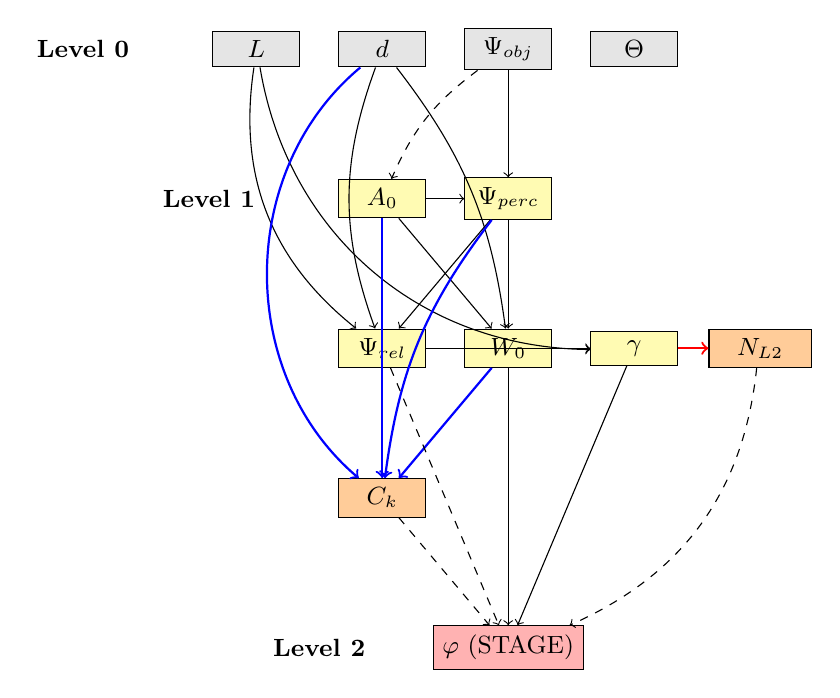
\begin{tikzpicture}[node distance=1.6cm, auto]
    % Level 0 nodes (ONLY 4: L, d, Psi_obj, Theta)
    \node[draw, rectangle, fill=gray!20, minimum width=1.1cm, font=\small] (L) {$L$};
    \node[draw, rectangle, fill=gray!20, minimum width=1.1cm, right of=L, font=\small] (d) {$d$};
    \node[draw, rectangle, fill=gray!20, minimum width=1.1cm, right of=d, font=\small] (Psiobj) {$\Psi_{\text{obj}}$};
    \node[draw, rectangle, fill=gray!20, minimum width=1.1cm, right of=Psiobj, font=\small] (Theta) {$\Theta$};

    % Level labels
    \node[left of=L, xshift=-0.6cm, font=\small] {\textbf{Level 0}};

    % Level 1 nodes (row 1: A0, Psi_perc)
    \node[draw, rectangle, fill=yellow!30, minimum width=1.1cm, below of=d, yshift=-0.3cm, font=\small] (A0) {$A_0$};
    \node[draw, rectangle, fill=yellow!30, minimum width=1.1cm, right of=A0, font=\small] (Psiperc) {$\Psi_{\text{perc}}$};

    % Level 1 nodes (row 2: Psi_rel, W0, gamma)
    \node[draw, rectangle, fill=yellow!30, minimum width=1.1cm, below of=A0, yshift=-0.3cm, font=\small] (Psirel) {$\Psi_{\text{rel}}$};
    \node[draw, rectangle, fill=yellow!30, minimum width=1.1cm, right of=Psirel, font=\small] (W0) {$W_0$};
    \node[draw, rectangle, fill=yellow!30, minimum width=1.1cm, right of=W0, font=\small] (gamma) {$\gamma$};

    % Level 1 nodes (row 3: N_L2 - HIERARCHY emerges from gamma!)
    \node[draw, rectangle, fill=orange!40, minimum width=1.3cm, right of=gamma, font=\small] (NL2) {$N_{L2}$};

    % Level 1 nodes (row 4: C_k - SEGMENT emerges from heterogeneity!)
    \node[draw, rectangle, fill=orange!40, minimum width=1.1cm, below of=Psirel, yshift=-0.3cm, font=\small] (Ck) {$C_k$};

    \node[left of=A0, xshift=-0.6cm, font=\small] {\textbf{Level 1}};

    % Level 2 node
    \node[draw, rectangle, fill=red!30, minimum width=1.8cm, below of=Ck, xshift=1.6cm, yshift=-0.3cm, font=\small] (phi) {$\varphi$ (STAGE)};
    \node[left of=phi, xshift=-0.8cm, font=\small] {\textbf{Level 2}};

    % Arrows Level 0 → Level 1
    \draw[->] (Psiobj) -- (Psiperc);
    \draw[->, dashed] (Psiobj) to[bend right=15] (A0);

    % Arrows within Level 1
    \draw[->] (A0) -- (Psiperc);
    \draw[->] (Psiperc) -- (Psirel);
    \draw[->] (L) to[bend right=30] (Psirel);
    \draw[->] (d) to[bend right=20] (Psirel);
    \draw[->] (A0) -- (W0);
    \draw[->] (Psiperc) -- (W0);
    \draw[->] (d) to[bend left=15] (W0);
    \draw[->] (Psirel) -- (gamma);
    \draw[->] (L) to[bend right=40] (gamma);

    % KEY: HIERARCHY (N_L2) emerges from gamma!
    \draw[->, thick, red] (gamma) -- (NL2);

    % KEY: SEGMENT (C_k) emerges from d, A_0, W_0, Psi!
    \draw[->, thick, blue] (d) to[bend right=50] (Ck);
    \draw[->, thick, blue] (A0) -- (Ck);
    \draw[->, thick, blue] (W0) -- (Ck);
    \draw[->, thick, blue] (Psiperc) to[bend right=15] (Ck);

    % Arrows Level 1 → Level 2
    \draw[->] (W0) -- (phi);
    \draw[->] (gamma) -- (phi);
    \draw[->, dashed] (Psirel) -- (phi);
    \draw[->, dashed] (NL2) to[bend left=30] (phi);
    \draw[->, dashed] (Ck) -- (phi);
\end{tikzpicture}
\end{center}

\textbf{Key Insights:}
\begin{itemize}[nosep]
    \item STAGE ($\varphi$) is the \textit{only} fully emergent 10C dimension
    \item Context ($\Psi$) splits into three layers: $\Psi_{\text{obj}} \rightarrow \Psi_{\text{perc}} \rightarrow \Psi_{\text{rel}}$
    \item \textbf{HIERARCHY ($N_{L2}$) emerges from complementarity ($\gamma$)} --- Chapter 15
    \item \textbf{SEGMENT ($C_k$) emerges from heterogeneity ($d, A_0, W_0, \Psi$)} --- Chapter 14
    \item Interventions can target any layer of $\Psi$, with different mechanisms
\end{itemize}

\end{tcolorbox}

\begin{tcolorbox}[colback=green!5!white, colframe=green!75!black,
    title=\textbf{Practical Implications of the Emergence Classification}]

\textbf{For Measurement:}
\begin{itemize}[nosep]
    \item \textbf{Fundamental (4):} Must be \textit{measured} or \textit{defined}---cannot be derived
    \item \textbf{Semi-Emergent (6):} Can be measured \textit{or} derived---cross-check possible
    \item \textbf{Fully Emergent (1):} Should be \textit{computed}---direct measurement is error-prone
\end{itemize}

\textbf{For Intervention Design:}
\begin{itemize}[nosep]
    \item Interventions targeting \textbf{Fundamental} dimensions directly change $\vec{S}_0$
    \item Interventions targeting \textbf{Semi-Emergent} dimensions may have indirect effects
    \item Interventions targeting \textbf{STAGE} are \textit{impossible}---you cannot directly target $\varphi$; you must change the inputs that generate it
\end{itemize}

\textbf{Example:} ``Move customer from Contemplation to Preparation'' is not a valid intervention target. Valid targets are:
\begin{itemize}[nosep]
    \item Increase $A_0$ (awareness) $\Rightarrow$ $\varphi$ emerges higher
    \item Increase $W_0$ (willingness) $\Rightarrow$ $\varphi$ emerges higher
    \item Change $\gamma$ (make complementary) $\Rightarrow$ $\varphi$ emerges higher
\end{itemize}

\end{tcolorbox}

%------------------------------------------------------------------------------
% Connection to P_eff (Chapter 16)
%------------------------------------------------------------------------------

\begin{tcolorbox}[colback=purple!5!white, colframe=purple!75!black,
    title=\textbf{Connection to $P_{\text{eff}}$: How Emergence Feeds the Final Output (Ch.16)}]

The 10C Emergence Classification is not merely theoretical---it directly determines the \textbf{Effective Probability of Behavior Change} ($P_{\text{eff}}$), the ultimate output of the EBF framework.

\textbf{The Master Equation (Chapter 16):}
\begin{equation}
\boxed{P_{\text{eff}} = \sigma(\text{WEC} \times \alpha_{\text{BCJ}} \times \beta_{\text{BCS}})}
\end{equation}

\textbf{How Emergence Feeds $P_{\text{eff}}$:}
\begin{center}
\renewcommand{\arraystretch}{1.3}
\begin{tabular}{@{}llll@{}}
\toprule
\textbf{Component} & \textbf{10C Source} & \textbf{Emergence Status} & \textbf{Role in $P_{\text{eff}}$} \\
\midrule
WEC & Ch.15 (HIERARCHY) & Semi-Emergent ($N_{L2}$) & Base probability \\
$\alpha_{\text{BCJ}}$ & STAGE ($\varphi$) & \textbf{Fully Emergent} & Journey-phase multiplier \\
$\beta_{\text{BCS}}$ & WHO ($C_k$) & \textbf{Semi-Emergent} & Segment multiplier \\
\bottomrule
\end{tabular}
\end{center}

\textbf{Critical Insight:} The two emergent dimensions become \textit{multipliers} in $P_{\text{eff}}$:
\begin{itemize}[nosep]
    \item $\alpha_{\text{BCJ}}$: Because STAGE ($\varphi$) is \textbf{Fully Emergent}, it must be \textit{computed} from $\vec{S}_0$---direct targeting is impossible
    \item $\beta_{\text{BCS}}$: Because Segment ($C_k$) is \textbf{Semi-Emergent}, it can be measured OR derived from heterogeneity $\mathcal{H}$
\end{itemize}

\textbf{Implication:} Interventions that correctly account for emergence (E-Full mode) will have more accurate $P_{\text{eff}}$ predictions than those using preset values (E-None mode).

\end{tcolorbox}


%#############################################################################
%#############################################################################
%  AXIOM SYSTEM: 4-SECTION ORGANIZATION
%#############################################################################
%#############################################################################

\begin{tcolorbox}[colback=red!5!white, colframe=red!75!black,
    title=\textbf{Paradigm Shift: From Primitive Types to Emergent Space}]

\textbf{Traditional View (Rejected):} There exist 8 discrete, primitive intervention types that form an ontological basis.

\textbf{Emergent View (This Appendix):} Interventions exist in a \textit{continuous 9-dimensional space}. Observed ``types'' are \textbf{empirical clusters}---regions of high density in this space where practical interventions tend to concentrate. They are \textit{heuristic shortcuts}, not theoretical primitives.

\textbf{Foundation:} This theory derives directly from Axiom A0 (``Zielgerichtetes Handeln unter Unsicherheit in Kontext'') through the 10C emergence chain:
\begin{equation}
\text{A0} \;\xrightarrow{\text{emergiert}}\; \text{10C} \;\xrightarrow{\text{emergiert}}\; \mathcal{I}_{\text{space}} \;\xrightarrow{\text{emergiert}}\; \text{A1--A8 Clusters}
\end{equation}
\end{tcolorbox}

%#############################################################################
%#############################################################################
% SECTION 1: FOUNDATIONS AND CLUSTERS
%#############################################################################
%#############################################################################

\section{Part 1: Foundations and Clusters (EIT-1, EIT-2, EIT-3)}
\label{sec:ie-part1-foundations}

\begin{tcolorbox}[colback=blue!5!white, colframe=blue!75!black,
    title=\textbf{Part 1 Overview: The Continuous Intervention Space}]

\textbf{Core Idea:} Interventions are not primitive categories. Instead:
\begin{enumerate}[nosep]
\item Interventions are **points** in a continuous 9-dimensional space $[0,1]^9$
\item Each point is an intervention vector $\vec{I}$ with 9 intensity components
\item Transformations between 9C status quo and post-intervention state are deterministic functions of $\vec{I}$
\item The optimal intervention vector emerges from context understanding
\end{enumerate}

\textbf{Three Axioms:}
\begin{itemize}[nosep]
\item **EIT-1:** Continuous space exists (mathematical structure)
\item **EIT-2:** Transformations follow 9C logic (functional form)
\item **EIT-3:** Clusters emerge naturally (empirical observation)
\end{itemize}

\end{tcolorbox}

\begin{tcolorbox}[colback=green!5!white, colframe=green!75!black,
    title=\textbf{✓ How This Appendix Is Structured (and Where to Start)}]

\textbf{If you want quick answers:}
\begin{itemize}[nosep]
\item \textbf{→ See next section:} MASTER MATRIX (one-page reference table)
\item \textbf{→ Then use:} Formula Reference (complete equations)
\end{itemize}

\textbf{If you want deep understanding:}
\begin{itemize}[nosep]
\item \textbf{→ Read:} Axioms EIT-1 through EIT-5 (Foundations, Journey, Horizon)
\item \textbf{→ Then read:} Axioms EIT-6 through EIT-8 (Universal Intensities)
\item \textbf{→ Then read:} Axioms EIT-9 through EIT-13 (Component Intensities)
\item \textbf{→ All validated against 4 Chapter 17 examples}
\end{itemize}

\textbf{Structure:} 13 axioms total = Emergence functions that compute every component of the intervention vector $\vec{I}$

\end{tcolorbox}

%%%%%%%%%%%%%%%%%%%%%%%%%%%%%%%%%%%%%%%%%%%%%%%%%%%%%%%%%%%%%%%%%%%%%%%%%%%%%%%
\subsection{★ MASTER MATRIX: Quick Lookup for All Emergence Functions ★}
%%%%%%%%%%%%%%%%%%%%%%%%%%%%%%%%%%%%%%%%%%%%%%%%%%%%%%%%%%%%%%%%%%%%%%%%%%%%%%%

\begin{table}[htbp]
\centering
\caption{Master Matrix: 8 Emergence Functions (EIT-6 through EIT-13)}
\label{tab:ie-master-matrix}
\small
\renewcommand{\arraystretch}{1.4}
\begin{tabular}{@{}lp{1.2cm}p{2.8cm}p{3cm}p{1.8cm}@{}}
\toprule
\textbf{Axiom} & \textbf{Comp.} & \textbf{Input Parameters} & \textbf{Core Principle} & \textbf{Deps} \\
\midrule
\textbf{EIT-6} & $I_{\text{AWARE}}$ & $A_0$ (awareness status) & Awareness NOT always problem & AU \\
\textbf{EIT-7} & $I_{\text{READY}}$ & $W_0, A_0$ & Willingness is bottleneck & AV \\
\textbf{EIT-8} & $I_{\text{WHEN}}$ & $\Psi, W_0$ (context) & Focus on changeable context & V \\
\midrule
\textbf{EIT-9} & $I_{\text{WHO}}$ & $L, L_{\text{goal}}$ (levels) & Level-shifting costs intensity & AAA \\
\textbf{EIT-10} & $I_{\text{WHAT}}$ & $d, d_{\text{goal}}, \gamma_d$ & Dimension targeting via $\gamma$ & C, B \\
\textbf{EIT-11} & $I_{\text{HOW}}$ & $\gamma_{\text{curr}}, \gamma_{\text{goal}}$ & Not all $\gamma$ reshapeable & B \\
\textbf{EIT-12} & $I_{\text{WHERE}}$ & $\Theta_k, D_{\text{suff}}$ & Data value $\neq$ volume & BBB \\
\textbf{EIT-13} & $I_{\text{HIER}}$ & Scope, urgency, resources & Scope-shift $\propto$ intensity & HI \\
\bottomrule
\end{tabular}
\end{table}

\textbf{Master Matrix Legend:}
\begin{itemize}[nosep]
\item \textbf{Axiom}: Reference (EIT-6 through EIT-13)
\item \textbf{Comp.}: Which $\vec{I}$ component this axiom computes
\item \textbf{Input Parameters}: What $\vec{S}_0$ data do you need to measure?
\item \textbf{Core Principle}: Single-sentence decision logic (the ``why'')
\item \textbf{Deps}: Which CORE Appendix is authoritative for input parameters?
\end{itemize}

\textbf{How to Use:}
\begin{enumerate}[nosep]
\item \textbf{Measure:} Gather all $\vec{S}_0$ inputs (9C Status Quo Vector)
\item \textbf{Lookup:} For each component $c$, find the corresponding Axiom in this matrix
\item \textbf{Apply:} Compute $I_c = f_c(\text{inputs from row})$ using the axiom's formula
\item \textbf{Combine:} Assemble $\vec{I}^* = (I_{\text{WHO}}^*, I_{\text{WHAT}}^*, \ldots, I_{\text{HIER}}^*)$
\item \textbf{Validate:} Check phase-affinity $\alpha(\vec{I}^*, \vec{S}_0)$ (Chapter 18)
\item \textbf{Deploy:} Use $\vec{I}^*$ as intervention design blueprint
\end{enumerate}

%======================================================================
% Formula Reference (all 8 functions, complete equations)
%======================================================================

\begin{table}[htbp]
\centering
\caption{Formula Reference: Complete Equations for All 8 Emergence Functions}
\label{tab:ie-formulas}
\footnotesize
\renewcommand{\arraystretch}{2}
\begin{tabular}{@{}lp{8cm}@{}}
\toprule
\textbf{Axiom} & \textbf{Complete Formula} \\
\midrule
\multicolumn{2}{l}{\textit{\textbf{Universal Intensities (EIT-6, 7, 8)}}} \\
\midrule
EIT-6 & $I_{\text{AWARE}} = f_{\text{AWARE}}(A_0)$ with piecewise cases based on awareness level \\
EIT-7 & $I_{\text{READY}} = f_{\text{READY}}(W_0, A_0)$ with piecewise cases based on willingness-awareness gap \\
EIT-8 & $I_{\text{WHEN}} = \max_c \{\text{leverage}_c(\Psi_c, W_0)\}$ with 4 cases for context changeability \\
\midrule
\multicolumn{2}{l}{\textit{\textbf{Component Intensities (EIT-9 through EIT-13)}}} \\
\midrule
EIT-9 & $I_{\text{WHO}} = f_{\text{WHO}}(L, L_{\text{goal}}, \text{available\_levers})$ with 6 cases for level-shifting \\
EIT-10 & $I_{\text{WHAT}:d} = f_{\text{WHAT}}(d_{\text{current}}, d_{\text{goal}}, \gamma_d)$ with 5 cases per dimension \\
EIT-11 & $I_{\text{HOW}} = f_{\text{HOW}}(\gamma_{\text{current}}, \gamma_{\text{goal}}, \text{feasibility})$ with 5 cases for reshaping \\
EIT-12 & $I_{\text{WHERE}} = f_{\text{WHERE}}(\Theta_{\text{known}}, \text{actionability}, \text{cost\_benefit})$ with 5 cases \\
EIT-13 & $I_{\text{HIERARCHY}} = f_{\text{HIERARCHY}}(\text{Scope}_c, \text{Scope}_g, \text{urgency}, \text{res})$ with 5 cases \\
\bottomrule
\end{tabular}
\end{table}

\textbf{Full Formula Sections:} For complete piecewise definitions with validation against Ch17 examples, see the individual axiom sections below (EIT-6 through EIT-13).

%------------------------------------------------------------------------------
\subsection{Axiom EIT-1: The Continuous Intervention Space}
\label{sec:ie-axiom-1}
%------------------------------------------------------------------------------

\begin{tcolorbox}[colback=blue!5!white, colframe=blue!75!black,
    title=\textbf{Axiom EIT-1: The Continuous Intervention Space}]

\textbf{Type:} structural (modeling decision)

\textbf{Statement:} An intervention $\mathcal{I}$ is a vector in a continuous 9-dimensional space:
\begin{equation}
\boxed{\vec{I} = (I_{\text{WHO}}, I_{\text{WHAT}}, I_{\text{HOW}}, I_{\text{WHEN}}, I_{\text{WHERE}}, I_{\text{AWARE}}, I_{\text{READY}}, I_{\text{STAGE}}, I_{\text{HIER}}) \in [0,1]^9}
\label{eq:ie-continuous-space}
\end{equation}

Where each component $I_c \in [0,1]$ represents the \textit{intensity} with which the intervention targets the corresponding 10C dimension:
\begin{itemize}[nosep]
    \item $I_c = 0$: Dimension $c$ is not targeted
    \item $I_c = 1$: Dimension $c$ is maximally targeted
    \item $I_c \in (0,1)$: Partial targeting with intermediate intensity
\end{itemize}

\textbf{Interpretation:} Every conceivable intervention occupies a point in $[0,1]^9$. There are no ``gaps'' or discrete categories in this space.
\end{tcolorbox}

%------------------------------------------------------------------------------
\subsection{Axiom EIT-2: Intervention as 9C Transformation}
\label{sec:ie-axiom-2}
\subsection{Axiom EIT-2: Intervention as 10C Transformation}
%------------------------------------------------------------------------------

\begin{tcolorbox}[colback=blue!5!white, colframe=blue!75!black,
    title=\textbf{Axiom EIT-2: Intervention as 10C Transformation}]

\textbf{Type:} structural (defines transformation mechanism)

\textbf{Statement:} An intervention transforms the Status Quo Vector through the intervention vector:
\begin{equation}
\boxed{\mathcal{I}(\vec{I}): \vec{S}_0 \mapsto \vec{S}_1 = \vec{S}_0 + \Delta\vec{S}(\vec{I})}
\label{eq:ie-transformation}
\end{equation}

Where the change vector $\Delta\vec{S}$ is a function of the intervention intensity:
\begin{equation}
\Delta S_c = f_c(I_c, \vec{S}_0, \Psi) \quad \text{for each dimension } c \in \{1, \ldots, 9\}
\end{equation}

\textbf{Note:} The transformation function $f_c$ depends on:
\begin{itemize}[nosep]
    \item The intervention intensity $I_c$
    \item The current state $\vec{S}_0$ (non-linear effects, ceiling effects)
    \item The context $\Psi$ (context-dependence of effectiveness)
\end{itemize}
\end{tcolorbox}

%------------------------------------------------------------------------------
\subsection{Axiom EIT-3: Cluster Emergence (Type Formation)}
\label{sec:ie-axiom-3}
%------------------------------------------------------------------------------

\begin{tcolorbox}[colback=blue!5!white, colframe=blue!75!black,
    title=\textbf{Axiom EIT-3: Cluster Emergence (Type Formation)}]

\textbf{Type:} theoretical (derived from EIT-1 + practical constraints)

\textbf{Statement:} In the continuous intervention space $[0,1]^9$, \textbf{empirical clusters} \textit{can} emerge due to:
\begin{enumerate}[nosep]
    \item \textbf{Practical constraints}: Real-world interventions cannot target all dimensions equally
    \item \textbf{Institutional path dependence}: Historical intervention designs cluster in certain regions
    \item \textbf{Cognitive accessibility}: Practitioners conceptualize interventions through familiar categories
    \item \textbf{Effectiveness peaks}: Certain configurations show higher average effectiveness
\end{enumerate}

\textbf{Formal Definition:} A cluster $\mathcal{C}_k$ is a region in $[0,1]^9$ with density $\rho(\vec{I})$ significantly above average:
\begin{equation}
\mathcal{C}_k = \left\{ \vec{I} \in [0,1]^9 \;\middle|\; \rho(\vec{I}) > \bar{\rho} + 2\sigma_\rho \right\}
\end{equation}

\textbf{Corollary:} The number of clusters $K$ is \textit{not} theoretically fixed. Empirically, $K \approx 8$ clusters are observed, but this is a contingent observation, not a theoretical necessity.
\end{tcolorbox}

\begin{tcolorbox}[colback=yellow!5!white, colframe=yellow!75!black,
    title=\textbf{Important: Cluster Labels in the EBF Framework}]

\textbf{Chapters 17--19:} Work exclusively in the \textbf{continuous intervention space} $[0,1]^9$. Interventions are described by their dominant $I_c$ components (e.g., ``$I_{\text{AWARE}} = 0.8$, $I_{\text{HOW}} = 0.3$''), \textit{not} by cluster labels.

\textbf{Chapter 20 only:} Introduces heuristic clusters \textbf{A1--A8} as practical shortcuts for:
\begin{itemize}[nosep]
    \item E-None mode (when context-specific parameters are unavailable)
    \item Stakeholder communication (discrete labels easier than vectors)
    \item Quick decisions (time pressure $<$ 1 hour)
\end{itemize}

\textbf{This appendix (IE):} Provides the \textit{theoretical foundation} explaining \textit{why} clusters emerge. It does \textbf{not} mandate their use---the continuous $I_c$ notation is primary.

\end{tcolorbox}

%#############################################################################
%#############################################################################
% SECTION 2: JOURNEY AND HORIZON EMERGENCE
%#############################################################################
%#############################################################################

\section{Part 2: Journey Position and Effect Horizon (EIT-4, EIT-5)}
\label{sec:ie-part2-journey-horizon}

\begin{tcolorbox}[colback=blue!5!white, colframe=blue!75!black,
    title=\textbf{Part 2 Overview: How $\vec{S}_0$ Emerges into Journey Position and Effect Horizon}]

\textbf{Core Idea:} Beyond the continuous intervention space itself, two critical quantities emerge \textit{deterministically} from the status quo:
\begin{enumerate}[nosep]
\item **Journey Position $\varphi$**: Where is the person/organization in their Behavioral Change Journey? (Unaware → Aware → Trigger → Action → Maintenance)
\item **Effect Horizon $\tau$**: Over what time-scale should we expect intervention effects to emerge? (Immediate → Short → Medium → Long-term)
\end{enumerate}

\textbf{Why This Matters:}
\begin{itemize}[nosep]
\item $\varphi = h(\vec{S}_0)$ explains why journey position is \textbf{not} a design choice but an \textbf{empirical fact}
\item $\tau = g(\vec{I})$ explains why some interventions are ``fast'' and others ``slow''
\item Together, they constrain which interventions are realistic (phase-affinity $\alpha$, Chapter 18)
\end{itemize}

\textbf{Two Axioms:}
\begin{itemize}[nosep]
\item **EIT-4:** Journey position emerges from status quo
\item **EIT-5:** Effect horizon emerges from intervention vector
\end{itemize}

\end{tcolorbox}

%------------------------------------------------------------------------------
\subsection{Axiom EIT-4: Journey-Position Emergence}
\label{sec:ie-axiom-4}
%------------------------------------------------------------------------------

\begin{tcolorbox}[colback=blue!5!white, colframe=blue!75!black,
    title=\textbf{Axiom EIT-4: Journey-Position Emergence}]

\textbf{Type:} structural (defines emergence function $h$)

\textbf{Statement:} The current position in the Behavioral Change Journey \textit{emerges} from the 10C Status Quo Vector, not from discrete phase labels:
\begin{equation}
\boxed{\varphi = h(\vec{S}_0) = h(L, d, \gamma, \Psi, \Theta, A_0, W_0, \text{Scope})}
\label{eq:ie-journey-emergence}
\end{equation}

\textbf{Key insight:} Journey phases (Awareness, Consideration, Preparation, Action, Consolidation) are \textit{regions} in the Status Quo space, not ontological categories. Boundaries are fuzzy.

\textbf{Derivation from 10C:}
\begin{itemize}[nosep]
    \item $A_0 < 0.3 \land W_0 < 0.2$ $\Rightarrow$ Unawareness region
    \item $A_0 > 0.5 \land W_0 < 0.4$ $\Rightarrow$ Contemplation region
    \item $A_0 > 0.7 \land W_0 > 0.6 \land \text{Scope} = L3$ $\Rightarrow$ Preparation region
    \item $W_0 > 0.8 \land \text{Scope} \geq L2$ $\Rightarrow$ Action region
    \item $W_0 > 0.9 \land \gamma_{\text{habit}} > 0.7$ $\Rightarrow$ Consolidation region
\end{itemize}
\end{tcolorbox}

%------------------------------------------------------------------------------
\subsection{Axiom EIT-5: Effect-Horizon Emergence}
\label{sec:ie-axiom-5}
%------------------------------------------------------------------------------

\begin{tcolorbox}[colback=blue!5!white, colframe=blue!75!black,
    title=\textbf{Axiom EIT-5: Effect-Horizon Emergence}]

\textbf{Type:} structural (defines emergence function $g$)

\textbf{Statement:} The temporal effect horizon $\tau$ of an intervention \textit{emerges} from the intervention vector, not from predetermined categories:
\begin{equation}
\boxed{\tau(\vec{I}) = g(I_{\text{HIER}}, I_{\text{WHO}}, I_{\text{HOW}})}
\label{eq:ie-horizon-emergence}
\end{equation}

\textbf{Effect-Horizon Mapping:}
\begin{itemize}[nosep]
    \item $I_{\text{HIER}} \approx 0$ (L3/operative) $\Rightarrow$ $\tau \in$ [Hours, Days] (Sofort)
    \item $I_{\text{HIER}} \approx 0.3$ (L2/tactical) $\Rightarrow$ $\tau \in$ [Days, Weeks] (Kurzfristig)
    \item $I_{\text{HIER}} \approx 0.6$ (L1/strategic) $\Rightarrow$ $\tau \in$ [Weeks, Months] (Mittelfristig)
    \item $I_{\text{HIER}} \approx 1$ (L0/system) $\Rightarrow$ $\tau \in$ [Months, Years] (Langfristig)
\end{itemize}

\textbf{Additional factors:}
\begin{itemize}[nosep]
    \item $I_{\text{WHO}}$ high (L4/society) $\Rightarrow$ increases $\tau$
    \item $I_{\text{HOW}}$ high ($\gamma$-restructuring) $\Rightarrow$ increases $\tau$
\end{itemize}
\end{tcolorbox}

%------------------------------------------------------------------------------
\subsection{Axiom EIT-6: Portfolio Composition}
%------------------------------------------------------------------------------

\begin{tcolorbox}[colback=blue!5!white, colframe=blue!75!black,
    title=\textbf{Axiom EIT-6: Portfolio Composition}]

\textbf{Type:} theoretical (derived from convex combination theory)

\textbf{Statement:} Multiple interventions combine through a \textit{portfolio function} that respects complementarity:
\begin{equation}
\boxed{P = \mathcal{F}(\vec{I}_1, \vec{I}_2, \ldots, \vec{I}_n; \Gamma) \quad \text{where } \Gamma = [\gamma_{ij}]}
\label{eq:ie-portfolio-composition}
\end{equation}

Where $\Gamma$ is the complementarity matrix governing interaction effects:
\begin{itemize}[nosep]
    \item $\gamma_{ij} > 0$: Interventions $i$ and $j$ are synergistic (super-additive)
    \item $\gamma_{ij} = 0$: Interventions are independent (additive)
    \item $\gamma_{ij} < 0$: Interventions crowd out each other (sub-additive)
\end{itemize}

\textbf{Key Insight:} Portfolio effect is \textit{not} simply the sum of individual effects:
\begin{equation}
P \neq \sum_{i} \text{Effect}(\vec{I}_i) \quad \text{unless } \gamma_{ij} = 0 \; \forall i,j
\end{equation}

\end{tcolorbox}

%------------------------------------------------------------------------------
\subsection{Axiom EIT-7: Phase-Type Affinity}
%------------------------------------------------------------------------------

\begin{tcolorbox}[colback=blue!5!white, colframe=blue!75!black,
    title=\textbf{Axiom EIT-7: Phase-Type Affinity}]

\textbf{Type:} empirical (requires evidence: Transtheoretical Model \citep{PAP-prochaska1992stages}, intervention timing research)

\textbf{Statement:} The effectiveness of an intervention type depends on the current journey phase through the \textbf{Phase-Type Affinity Matrix} $\alpha_{\text{BCJ}}$:
\begin{equation}
\boxed{\alpha_{\text{BCJ}}(T_k, \varphi_j) \in [0,1] \quad \text{for intervention type } T_k \text{ in phase } \varphi_j}
\label{eq:ie-phase-affinity}
\end{equation}

\textbf{Interpretation:}
\begin{itemize}[nosep]
    \item $\alpha > 0.7$: Type $T_k$ is highly effective in phase $\varphi_j$
    \item $\alpha \in [0.3, 0.7]$: Moderate effectiveness
    \item $\alpha < 0.3$: Type $T_k$ is ineffective or counterproductive in phase $\varphi_j$
\end{itemize}

\textbf{Example:} Commitment devices (high $I_{\text{HOW}}$) have high $\alpha$ in Preparation/Action phases ($\alpha \approx 0.75$) but low $\alpha$ in Unawareness ($\alpha \approx 0.15$).

\end{tcolorbox}

%------------------------------------------------------------------------------
\subsection{Axiom EIT-8: Segment Multiplier}
%------------------------------------------------------------------------------

\begin{tcolorbox}[colback=blue!5!white, colframe=blue!75!black,
    title=\textbf{Axiom EIT-8: Segment Multiplier}]

\textbf{Type:} empirical (requires evidence: treatment effect heterogeneity literature \citep{athey2016recursive})

\textbf{Statement:} Intervention effectiveness is modulated by behavioral segment through the \textbf{Segment Multiplier Matrix} $\beta_{\text{BCS}}$:
\begin{equation}
\boxed{\beta_{\text{BCS}}(T_k, C_s) \in \mathbb{R} \quad \text{for intervention type } T_k \text{ on segment } C_s}
\label{eq:ie-segment-multiplier}
\end{equation}

\textbf{Critical:} Unlike $\alpha$, segment multipliers can be negative (backfire effects):
\begin{itemize}[nosep]
    \item $\beta > 1.3$: Strong positive multiplier
    \item $\beta \in [0.7, 1.3]$: Near-neutral effect
    \item $\beta \in [0, 0.7]$: Attenuated effect
    \item $\beta < 0$: \textbf{Backfire risk} --- intervention has opposite effect
\end{itemize}

\textbf{Example:} Financial incentives (high $I_{\text{WHAT},F}$) on autonomy-seeking segments can have $\beta < 0$ due to crowding-out of intrinsic motivation.

\end{tcolorbox}

%------------------------------------------------------------------------------
\subsection{Axiom EIT-9: Crowding-Out Constraint}
%------------------------------------------------------------------------------

\begin{tcolorbox}[colback=blue!5!white, colframe=blue!75!black,
    title=\textbf{Axiom EIT-9: Crowding-Out Constraint}]

\textbf{Type:} empirical (evidence: \citep{frey1997motivation, deci1971effects, gneezy2000pay})

\textbf{Statement:} Certain intervention dimension combinations exhibit \textit{systematic} negative complementarity:
\begin{equation}
\boxed{\gamma(I_{\text{WHO},o}, I_{\text{WHAT},F}) < 0 \quad \text{and} \quad \gamma(I_{\text{WHAT},F}, I_{\text{HOW}}) < 0}
\label{eq:ie-crowding-out}
\end{equation}

\textbf{Theoretical Foundation:}
\begin{itemize}[nosep]
    \item $\gamma(\text{Social}, \text{Financial}) \approx -0.2$: Social norms ($I_{\text{WHO},o}$) + Financial incentives ($I_{\text{WHAT},F}$) --- extrinsic rewards undermine social motivation \citep{frey1997motivation}
    \item $\gamma(\text{Financial}, \text{Commitment}) \approx -0.3$: Financial ($I_{\text{WHAT},F}$) + Commitment ($I_{\text{HOW}}$) --- external rewards undermine internal commitment \citep{deci1971effects}
\end{itemize}

\textbf{Design Implication:} Portfolios with high intensity on both (Social + Financial) or (Financial + Commitment) require explicit justification and crowding-out mitigation strategies.

\end{tcolorbox}

%------------------------------------------------------------------------------
\subsection{Axiom EIT-10: Data-Mode Correspondence}
%------------------------------------------------------------------------------

\begin{tcolorbox}[colback=blue!5!white, colframe=blue!75!black,
    title=\textbf{Axiom EIT-10: Data-Mode Correspondence}]

\textbf{Type:} structural (design rule linking data quality to method choice)

\textbf{Statement:} The feasible emergence mode is \textit{determined} by data sufficiency:
\begin{equation}
\boxed{
\text{Mode}(D_{\text{suff}}) = \begin{cases}
\text{E-Full} & \text{if } D_{\text{suff}} > 0.7 \\
\text{E-Partial} & \text{if } 0.4 \leq D_{\text{suff}} \leq 0.7 \\
\text{E-None} & \text{if } D_{\text{suff}} < 0.4
\end{cases}
}
\label{eq:ie-data-mode}
\end{equation}

\textbf{Corollary:} Mode selection is \textit{not} a design preference; it is constrained by epistemic limitations.

\end{tcolorbox}

%------------------------------------------------------------------------------
\subsection{Axiom EIT-11: Effective Probability}
%------------------------------------------------------------------------------

\begin{tcolorbox}[colback=blue!5!white, colframe=blue!75!black,
    title=\textbf{Axiom EIT-11: Effective Probability of Behavior Change}]

\textbf{Type:} structural (definitional: aggregation formula for $P_{\text{eff}}$)

\textbf{Statement:} The effective probability of behavior change emerges from the 10C system through:
\begin{equation}
\boxed{P_{\text{eff}} = \sigma(\text{WEC} \times \alpha_{\text{BCJ}} \times \beta_{\text{BCS}})}
\label{eq:ie-peff}
\end{equation}

Where:
\begin{itemize}[nosep]
    \item $\sigma(\cdot)$: Sigmoid function mapping to $[0,1]$
    \item WEC: Weighted Effectiveness Coefficient (from HIERARCHY, Chapter 15)
    \item $\alpha_{\text{BCJ}}$: Phase-Type Affinity (Axiom EIT-7)
    \item $\beta_{\text{BCS}}$: Segment Multiplier (Axiom EIT-8)
\end{itemize}

\textbf{Key Insight:} $P_{\text{eff}}$ is the \textit{ultimate output} of the 10C framework---all other computations feed into this probability.

\end{tcolorbox}

%------------------------------------------------------------------------------
\subsection{Axiom EIT-12: 10C Dimensional Decomposition}
%------------------------------------------------------------------------------

\begin{tcolorbox}[colback=blue!5!white, colframe=blue!75!black,
    title=\textbf{Axiom EIT-12: 10C Dimensional Decomposition}]

\textbf{Type:} structural (the 10C dimensions are the true primitives)

\textbf{Statement:} Any intervention $\vec{I}$ is represented as a vector in the continuous 10C space:
\begin{equation}
\boxed{\vec{I} = (I_{\text{WHO}}, I_{\text{WHAT}}, I_{\text{HOW}}, I_{\text{WHEN}}, I_{\text{WHERE}}, I_{\text{AWARE}}, I_{\text{READY}}, I_{\text{STAGE}}, I_{\text{HIER}}) \in [0,1]^9}
\label{eq:ie-10c-decomp}
\end{equation}

\textbf{The 9 Dimensional Primitives:}
\begin{center}
\renewcommand{\arraystretch}{1.2}
\begin{tabular}{@{}llll@{}}
\toprule
\textbf{Dim.} & \textbf{Name} & \textbf{Target Component} & \textbf{Mechanisms} \\
\midrule
WHO & Level & Decision unit & Individual, household, group, community \\
WHAT & Utility & $u_F, u_S, u_X$ & Financial, social, self-concept incentives \\
HOW & Interaction & $\gamma_{ij}$ & Pre-commitment, bundling, sequencing \\
WHEN & Context & $\kappa_{\text{KON}}$ & Choice architecture, defaults, timing \\
WHERE & Environment & Physical/digital & Channel, location, platform \\
AWARE & Awareness & $A(\cdot)$ & Information, salience, feedback \\
READY & Willingness & $W_{\text{base}}, \theta$ & Motivation, capacity, threshold \\
STAGE & Phase & $\varphi$ & Journey-appropriate messaging \\
HIER & Scope & $L_0$--$L_3$ & Operative, tactical, strategic \\
\bottomrule
\end{tabular}
\end{center}

\textbf{Corollary:} The optimal vector $\vec{I}^*$ emerges from context understanding via $f(\beta, \lambda, \theta, W_{\text{base}}, \varphi, \Psi, L)$.

\end{tcolorbox}

%------------------------------------------------------------------------------
\subsection{Axiom EIT-13: Temporal Consistency}
%------------------------------------------------------------------------------

\begin{tcolorbox}[colback=blue!5!white, colframe=blue!75!black,
    title=\textbf{Axiom EIT-13: Temporal Consistency}]

\textbf{Type:} theoretical (derived from portfolio coherence requirements)

\textbf{Statement:} Portfolio effect horizons must be temporally consistent:
\begin{equation}
\boxed{\tau(P) = \min\{\tau(\vec{I}_i)\} \cdot \xi(\tau_{\text{spread}})}
\label{eq:ie-temporal-consistency}
\end{equation}

Where $\xi$ is a coherence penalty for portfolios with divergent effect horizons:
\begin{itemize}[nosep]
    \item $\xi = 1$ if all $\tau(\vec{I}_i)$ are in same category
    \item $\xi < 1$ if horizons span multiple categories (incoherence penalty)
\end{itemize}

\textbf{Design Implication:} Avoid mixing ``immediate'' (hours) and ``long-term'' (years) interventions without explicit sequencing strategy.

\end{tcolorbox}

%------------------------------------------------------------------------------
\subsection{Axiom EIT-14: Segment Emergence}
%------------------------------------------------------------------------------

\begin{tcolorbox}[colback=blue!5!white, colframe=blue!75!black,
    title=\textbf{Axiom EIT-14: Segment Emergence from Heterogeneity}]

\textbf{Type:} theoretical (derived from Chapter 14 heterogeneity theory \citep{athey2016recursive, wager2018estimation})

\textbf{Statement:} Behavioral segments \textit{emerge} from population heterogeneity rather than being imposed:
\begin{equation}
\boxed{C_k = f(\mathcal{H}, \Psi) \quad \text{where } \mathcal{H} = \{(\vec{\omega}_i, A_i, W_i)\}_{i=1}^{N}}
\label{eq:ie-segment-emergence}
\end{equation}

\textbf{Key Insight (Chapter 14):} The number of segments $k^*$ is context-dependent, not fixed. Segmentation emerges from:
\begin{itemize}[nosep]
    \item $\vec{\omega}_i$: Individual utility weights (WHAT)
    \item $A_i$: Individual awareness levels (AWARE)
    \item $W_i$: Individual willingness thresholds (READY)
    \item $\Psi$: Context that activates different response patterns (WHEN)
\end{itemize}

\textbf{Corollary:} The ``right'' number of segments cannot be determined a priori---it emerges from data.

\end{tcolorbox}

%------------------------------------------------------------------------------
\subsection{Axiom EIT-15: General Complementarity Function}
%------------------------------------------------------------------------------

\begin{tcolorbox}[colback=blue!5!white, colframe=blue!75!black,
    title=\textbf{Axiom EIT-15: General Complementarity Function}]

\textbf{Type:} structural (mathematical: defines $\gamma$ as continuous function with symmetry properties)

\textbf{Statement:} Complementarity between interventions is a continuous function of the intervention vectors:
\begin{equation}
\boxed{\gamma: [0,1]^9 \times [0,1]^9 \rightarrow [-1, 1] \quad \text{with } \gamma(\vec{I}, \vec{I}) = 0}
\label{eq:ie-general-gamma}
\end{equation}

\textbf{Properties:}
\begin{itemize}[nosep]
    \item \textbf{Symmetry:} $\gamma(\vec{I}_1, \vec{I}_2) = \gamma(\vec{I}_2, \vec{I}_1)$
    \item \textbf{Self-neutrality:} $\gamma(\vec{I}, \vec{I}) = 0$ (no self-interaction)
    \item \textbf{Context-dependence:} $\gamma = \gamma(\vec{I}_1, \vec{I}_2; \Psi, C_k)$
    \item \textbf{Bounded:} $|\gamma| \leq 1$ ensures tractable portfolio optimization
\end{itemize}

\textbf{Approximation:} For practical computation, the discrete matrix $\gamma_{ij}$ (T-type to T-type) approximates $\gamma(\vec{I}_1, \vec{I}_2)$ when interventions are dominated by single types.

\end{tcolorbox}


%%%%%%%%%%%%%%%%%%%%%%%%%%%%%%%%%%%%%%%%%%%%%%%%%%%%%%%%%%%%%%%%%%%%%%%%%%%%%%%
\section{Theorem System: Emergent Intervention Theory}
\label{sec:ie-theorems}
%%%%%%%%%%%%%%%%%%%%%%%%%%%%%%%%%%%%%%%%%%%%%%%%%%%%%%%%%%%%%%%%%%%%%%%%%%%%%%%

The axioms above generate the following theorems through logical derivation.

%------------------------------------------------------------------------------
\subsection{Theorem IE-T1: Intervention Space Completeness}
%------------------------------------------------------------------------------

\begin{tcolorbox}[colback=green!5!white, colframe=green!75!black,
    title=\textbf{Theorem IE-T1: Intervention Space Completeness}]

\textbf{Statement:} The continuous intervention space $[0,1]^9$ is \textbf{complete}: every conceivable behavioral intervention can be represented as a point in this space.

\textbf{Proof Sketch:}
\begin{enumerate}[nosep]
    \item By Axiom EIT-1, interventions are vectors $\vec{I} \in [0,1]^9$
    \item The 9 dimensions correspond to the 9 CORE dimensions (WHO through HIERARCHY)
    \item Any intervention must target at least one aspect of behavior
    \item All behavioral aspects are captured by the 10C framework (by construction)
    \item Therefore, any intervention has a representation in $[0,1]^9$ \qed
\end{enumerate}

\textbf{Corollary:} Interventions that appear ``novel'' are merely previously unoccupied regions of $[0,1]^9$.

\end{tcolorbox}

%------------------------------------------------------------------------------
\subsection{Theorem IE-T2: Cluster Emergence}
%------------------------------------------------------------------------------

\begin{tcolorbox}[colback=green!5!white, colframe=green!75!black,
    title=\textbf{Theorem IE-T2: Cluster Emergence from Practice}]

\textbf{Statement:} High-density clusters in $[0,1]^9$ emerge necessarily from practical constraints, regardless of theoretical framework.

\textbf{Proof Sketch:}
\begin{enumerate}[nosep]
    \item Real-world interventions have resource constraints (time, budget, expertise)
    \item Resource constraints favor interventions with few dominant $I_c$ components
    \item Dominant-component interventions cluster around axis-aligned regions
    \item Historical path dependence reinforces successful configurations
    \item Therefore, clusters emerge regardless of intentional design \qed
\end{enumerate}

\textbf{Implication:} The 8 clusters (A1--A8) observed empirically are not arbitrary---they reflect structural constraints on intervention design.

\end{tcolorbox}

%------------------------------------------------------------------------------
\subsection{Theorem IE-T3: Journey Position Derivation}
%------------------------------------------------------------------------------

\begin{tcolorbox}[colback=green!5!white, colframe=green!75!black,
    title=\textbf{Theorem IE-T3: Journey Position is Fully Determined}]

\textbf{Statement:} Given complete knowledge of the Status Quo Vector $\vec{S}_0$, the journey position $\varphi$ is \textbf{uniquely determined}.

\textbf{Formal Statement:}
\begin{equation}
\vec{S}_0 = \vec{S}_0' \implies \varphi(\vec{S}_0) = \varphi(\vec{S}_0')
\end{equation}

\textbf{Proof:}
\begin{enumerate}[nosep]
    \item By Axiom EIT-4, $\varphi = h(\vec{S}_0)$ where $h$ is a function
    \item Functions are deterministic: same input $\Rightarrow$ same output
    \item Therefore, identical Status Quo Vectors yield identical journey positions \qed
\end{enumerate}

\textbf{Corollary:} Disagreement about journey position implies disagreement about some $\vec{S}_0$ component---resolve the latter to resolve the former.

\end{tcolorbox}

%------------------------------------------------------------------------------
\subsection{Theorem IE-T5: Data Sufficiency Determines Feasibility}
%------------------------------------------------------------------------------

\begin{tcolorbox}[colback=green!5!white, colframe=green!75!black,
    title=\textbf{Theorem IE-T5: Data Sufficiency Determines Mode Feasibility}]

\textbf{Statement:} The maximum achievable precision in emergence is bounded by data sufficiency:
\begin{equation}
\text{Precision}(\vec{I}^*) \leq f(D_{\text{suff}})
\end{equation}

Where $f$ is monotonically increasing in $D_{\text{suff}}$.

\textbf{Proof Sketch:}
\begin{enumerate}[nosep]
    \item Emergence functions propagate uncertainty from inputs to outputs
    \item Input uncertainty is inversely related to $D_{\text{suff}}$
    \item Output uncertainty (inverse of precision) inherits input uncertainty
    \item Therefore, low $D_{\text{suff}} \Rightarrow$ low precision \qed
\end{enumerate}

\textbf{Implication:} There is no ``free lunch''---high-precision emergence requires high-quality data.

\end{tcolorbox}

%------------------------------------------------------------------------------
\subsection{Theorem IE-T6: Portfolio Optimization}
%------------------------------------------------------------------------------

\begin{tcolorbox}[colback=green!5!white, colframe=green!75!black,
    title=\textbf{Theorem IE-T6: Optimal Portfolio Existence}]

\textbf{Statement:} For any target behavior change and resource constraint, an optimal portfolio $P^*$ exists in the continuous intervention space.

\textbf{Formal Statement:}
\begin{equation}
P^* = \arg\max_P \; P_{\text{eff}}(P) \quad \text{s.t. } \text{Cost}(P) \leq B, \; P \subset [0,1]^9
\end{equation}

\textbf{Proof Sketch:}
\begin{enumerate}[nosep]
    \item $[0,1]^9$ is compact (closed and bounded)
    \item $P_{\text{eff}}(\cdot)$ is continuous (by Axiom EIT-11)
    \item Weierstrass theorem: continuous function on compact set achieves maximum
    \item Therefore, $P^*$ exists \qed
\end{enumerate}

\textbf{Note:} Existence does not imply computability---finding $P^*$ may require optimization algorithms.

\end{tcolorbox}

%------------------------------------------------------------------------------
\subsection{Theorem IE-T7: Phase-Affinity Monotonicity}
%------------------------------------------------------------------------------

\begin{tcolorbox}[colback=green!5!white, colframe=green!75!black,
    title=\textbf{Theorem IE-T7: Phase-Affinity Structure}]

\textbf{Statement:} The Phase-Type Affinity Matrix $\alpha_{\text{BCJ}}$ exhibits systematic structure: each intervention type has a characteristic phase profile.

\textbf{Formal Pattern:}
\begin{itemize}[nosep]
    \item \textbf{High $I_{\text{AWARE}}$ (Awareness):} Peak in Unawareness/Contemplation, decline in Action/Maintenance
    \item \textbf{High $I_{\text{HOW}}$ (Commitment):} Peak in Preparation/Action, low in Unawareness
    \item \textbf{High $I_{\text{WHEN}}$ (Contextual):} Relatively flat across phases (universal applicability)
    \item \textbf{High $I_{\text{WHAT},F}$ (Financial):} Peak in Action, potential backfire in Maintenance (crowding-out)
\end{itemize}

\textbf{Derivation:} These patterns emerge from the theoretical mechanisms of each type interacting with the psychological characteristics of each phase.

\end{tcolorbox}

%------------------------------------------------------------------------------
\subsection{Theorem IE-T8: Segment Response Heterogeneity}
%------------------------------------------------------------------------------

\begin{tcolorbox}[colback=green!5!white, colframe=green!75!black,
    title=\textbf{Theorem IE-T8: Segment Response Heterogeneity}]

\textbf{Statement:} Different behavioral segments respond differently to the same intervention:
\begin{equation}
\beta_{\text{BCS}}(T_k, C_s) \neq \beta_{\text{BCS}}(T_k, C_{s'}) \quad \text{for } s \neq s'
\end{equation}

\textbf{Proof:}
\begin{enumerate}[nosep]
    \item Segments differ in $(\vec{\omega}, A, W)$ by definition (Axiom EIT-14)
    \item Intervention effectiveness depends on alignment with $\vec{\omega}$
    \item Different $\vec{\omega} \Rightarrow$ different response to same $T_k$
    \item Therefore, $\beta$ varies by segment \qed
\end{enumerate}

\textbf{Implication:} ``One-size-fits-all'' interventions are suboptimal; segment-specific tailoring increases $P_{\text{eff}}$.

\end{tcolorbox}

%------------------------------------------------------------------------------
\subsection{Theorem IE-T9: Crowding-Out Universality}
%------------------------------------------------------------------------------

\begin{tcolorbox}[colback=green!5!white, colframe=green!75!black,
    title=\textbf{Theorem IE-T9: Crowding-Out is Context-Invariant}]

\textbf{Statement:} The sign of $\gamma(T_6, T_7)$ and $\gamma(T_7, T_8)$ is negative across contexts:
\begin{equation}
\gamma(T_6, T_7; \Psi) < 0 \quad \forall \Psi \quad \text{(social-financial crowding-out)}
\end{equation}

\textbf{Derivation:}
\begin{enumerate}[nosep]
    \item Financial incentives (high $I_{\text{WHAT},F}$) signal that the desired behavior is costly/unpleasant
    \item This signal undermines social motivation (high $I_{\text{WHO},o}$) by making it ``transactional''
    \item The signaling mechanism is psychological, not context-dependent
    \item Therefore, crowding-out persists across contexts (though magnitude varies) \qed
\end{enumerate}

\textbf{Meta-Analytic Evidence:} \citet{frey1997motivation}, \citet{deci1971effects}, \citet{gneezy2000pay}

\end{tcolorbox}

%------------------------------------------------------------------------------
\subsection{Theorem IE-T10: $P_{\text{eff}}$ Emergence}
%------------------------------------------------------------------------------

\begin{tcolorbox}[colback=green!5!white, colframe=green!75!black,
    title=\textbf{Theorem IE-T10: $P_{\text{eff}}$ Emerges from 10C}]

\textbf{Statement:} The effective probability of behavior change is fully determined by the 10C Status Quo Vector and the intervention vector:
\begin{equation}
P_{\text{eff}} = P_{\text{eff}}(\vec{S}_0, \vec{I})
\end{equation}

\textbf{Proof:}
\begin{enumerate}[nosep]
    \item By Axiom EIT-11: $P_{\text{eff}} = \sigma(\text{WEC} \times \alpha_{\text{BCJ}} \times \beta_{\text{BCS}})$
    \item WEC depends on $\vec{S}_0$ (via HIERARCHY emergence from $\gamma$)
    \item $\alpha_{\text{BCJ}}$ depends on $\varphi$ (Axiom EIT-7), which depends on $\vec{S}_0$ (Axiom EIT-4)
    \item $\beta_{\text{BCS}}$ depends on $C_k$ (Axiom EIT-8), which depends on $\vec{S}_0$ (Axiom EIT-14)
    \item $\vec{I}$ determines which $T_k$ are active
    \item Therefore, $P_{\text{eff}}$ is a function of $(\vec{S}_0, \vec{I})$ only \qed
\end{enumerate}

\end{tcolorbox}

%------------------------------------------------------------------------------
\subsection{Theorem IE-T11: Mode Selection Optimality}
%------------------------------------------------------------------------------

\begin{tcolorbox}[colback=green!5!white, colframe=green!75!black,
    title=\textbf{Theorem IE-T11: Mode Selection Minimizes Expected Error}]

\textbf{Statement:} The mode selection rule (Axiom EIT-10) minimizes expected decision error:
\begin{equation}
\text{Mode}^* = \arg\min_m \; \mathbb{E}[\text{Error}(m, D_{\text{suff}})]
\end{equation}

\textbf{Intuition:}
\begin{itemize}[nosep]
    \item E-Full with low $D_{\text{suff}}$: False precision (overconfident point estimates)
    \item E-None with high $D_{\text{suff}}$: Wasted information (heuristics despite good data)
    \item Matching mode to data quality minimizes both types of error
\end{itemize}

\textbf{Derivation:} Bayesian decision theory with quadratic loss function.

\end{tcolorbox}

%------------------------------------------------------------------------------
\subsection{Theorem IE-T12: Uncertainty Propagation}
%------------------------------------------------------------------------------

\begin{tcolorbox}[colback=green!5!white, colframe=green!75!black,
    title=\textbf{Theorem IE-T12: Uncertainty Propagation through Emergence}]

\textbf{Statement:} Uncertainty in emergence outputs is bounded by uncertainty in inputs:
\begin{equation}
\text{Var}(\varphi) \leq \sum_c \left(\frac{\partial h}{\partial S_{0,c}}\right)^2 \text{Var}(S_{0,c})
\end{equation}

\textbf{Proof:} Delta method (first-order Taylor approximation) applied to emergence function $h$.

\textbf{Implication:} To reduce output uncertainty, focus on reducing uncertainty in high-sensitivity inputs (those with large $\frac{\partial h}{\partial S_{0,c}}$).

\end{tcolorbox}

% Note: Theorem IE-T4 (Confidence-Weighted Decision Rule) appears in Section~\ref{sec:ie-weak-priors}


%%%%%%%%%%%%%%%%%%%%%%%%%%%%%%%%%%%%%%%%%%%%%%%%%%%%%%%%%%%%%%%%%%%%%%%%%%%%%%%
\section{Emergence Modes: E-Full, E-Partial, E-None}
\label{sec:ie-emergence-modes}
%%%%%%%%%%%%%%%%%%%%%%%%%%%%%%%%%%%%%%%%%%%%%%%%%%%%%%%%%%%%%%%%%%%%%%%%%%%%%%%

\begin{tcolorbox}[colback=red!5!white, colframe=red!75!black,
    title=\textbf{Critical: The Emergence-Data Interaction}]

The Emergent Intervention Theory allows interventions to emerge from $\vec{S}_0$. However, this emergence \textbf{requires data}. The fundamental design choice is: \textbf{What do we let emerge versus what do we preset?}

This choice is \textit{not} a pure preference---it is \textbf{constrained by data availability}.
\end{tcolorbox}

%------------------------------------------------------------------------------
\subsection{The Three Emergence Modes}
\label{sec:ie-three-modes}
%------------------------------------------------------------------------------

\begin{tcolorbox}[colback=blue!5!white, colframe=blue!75!black,
    title=\textbf{Definition IE-D1: Emergence Modes (E-Full, E-Partial, E-None)}]

\textbf{E-Full (Pure Emergence):} Everything emerges from $\vec{S}_0$:
\begin{equation}
\vec{S}_0 \xrightarrow{h} \varphi \xrightarrow{g} \tau \xrightarrow{\alpha(\cdot)} \vec{I}^* \xrightarrow{\gamma(\cdot,\cdot)} P^*
\end{equation}
\begin{itemize}[nosep]
    \item Journey position $\varphi$ emerges from Status Quo
    \item Effect horizon $\tau$ emerges from intervention vector
    \item Phase-affinity $\alpha(\vec{I}, \vec{S}_0)$ computed continuously
    \item Complementarity $\gamma(\vec{I}_i, \vec{I}_j)$ computed continuously
    \item Segment-multiplier $\sigma_s$ emerges from (Intervention, Segment) pair
\end{itemize}

\textbf{E-Partial (Hybrid Emergence):} Some elements emerge, others are preset:
\begin{equation}
\vec{S}_0 \xrightarrow{h} \varphi, \tau \quad + \quad \gamma_{ij}^{\text{Literatur}} \xrightarrow{\text{optimize}} P^*
\end{equation}
\begin{itemize}[nosep]
    \item Journey position $\varphi$ and effect horizon $\tau$ emerge
    \item Complementarity $\gamma_{ij}$ taken from literature (BBB)
    \item Segment-multiplier $\sigma_s$ taken from literature or LLMMC
\end{itemize}

\textbf{E-None (Heuristic):} Nothing emerges, everything is preset:
\begin{equation}
\text{Context} \xrightarrow{\text{Rule}} A_k \xrightarrow{\gamma_{ij}^{\text{preset}}} P
\end{equation}
\begin{itemize}[nosep]
    \item Intervention selected from preset clusters A1--A8
    \item Complementarity matrix $\gamma_{ij}$ is preset
    \item Portfolio archetypes applied without optimization
\end{itemize}
\end{tcolorbox}

\begin{table}[htbp]
\centering
\caption{Emergence Modes: What Emerges vs.\ What Is Preset}
\label{tab:ie-emergence-modes}
\renewcommand{\arraystretch}{1.3}
\begin{tabular}{@{}lcccccc@{}}
\toprule
\textbf{Mode} & $\varphi$ & $\tau$ & $\alpha$ & $\sigma_s$ & $\gamma$ & $P^*$ \\
\midrule
\textbf{E-Full} & Emerges & Emerges & Emerges & Emerges & Emerges & Optimal \\
\textbf{E-Partial} & Emerges & Emerges & Preset & Preset & Preset & Near-Optimal \\
\textbf{E-None} & Preset & Preset & Preset & Preset & Preset & Heuristic \\
\bottomrule
\end{tabular}
\end{table}


%%%%%%%%%%%%%%%%%%%%%%%%%%%%%%%%%%%%%%%%%%%%%%%%%%%%%%%%%%%%%%%%%%%%%%%%%%%%%%%
\section{Data Sources and Confidence Levels}
\label{sec:ie-data-sources}
%%%%%%%%%%%%%%%%%%%%%%%%%%%%%%%%%%%%%%%%%%%%%%%%%%%%%%%%%%%%%%%%%%%%%%%%%%%%%%%

\begin{tcolorbox}[colback=yellow!5!white, colframe=yellow!75!black,
    title=\textbf{Key Insight: Data Source Determines Emergence Feasibility}]

Different data sources enable different levels of confidence in emergence. The \textbf{8-Level Prior Hierarchy} formalizes this relationship:

\begin{center}
\renewcommand{\arraystretch}{1.3}
\begin{tabular}{@{}lccl@{}}
\toprule
\textbf{Data Source} & \textbf{$C$} & \textbf{Mode} & \textbf{Description} \\
\midrule
Empirical (RCT, Survey, Behavioral) & $1.0$ & E-Full & Direct measurement \\
LLMMC (LLM Monte Carlo) & $0.7$ & E-Full & LLM aggregates 1000s of papers \\
Literature (BBB, Meta-Analysis) & $0.5$ & E-Partial & Published studies \\
\textbf{Expert-Crowd} ($n > 10$) & $0.45$ & E-Partial & Aggregated expert estimates \\
Expert (Single) & $0.2$ & E-Partial & One domain specialist \\
\textbf{Lay-Crowd} ($n > 30$) & $0.15$ & E-None & Aggregated non-experts \\
\textbf{Lay (Single)} & $0.05$ & E-None & Non-expert with BE biases \\
\textbf{Random (Uninformed)} & $0.0$ & E-None & Uniform prior, no information \\
\bottomrule
\end{tabular}
\end{center}

\textbf{Critical:} LLMMC democratizes E-Full! Even without expensive surveys, emergence is possible with $C = 0.7$.
\end{tcolorbox}

%------------------------------------------------------------------------------
\subsection{The 8-Level Prior Hierarchy: Definitions}
\label{sec:ie-prior-hierarchy}
%------------------------------------------------------------------------------

\begin{tcolorbox}[colback=blue!5!white, colframe=blue!75!black,
    title=\textbf{Definition IE-D2: The 8-Level Prior Hierarchy}]

\textbf{Level 1: Empirical} ($C = 1.0$): Direct measurement through RCT, survey, or behavioral observation. Gold standard for causal inference.

\textbf{Level 2: LLMMC} ($C = 0.7$): LLM Monte Carlo estimation aggregating information from thousands of scientific papers. Higher than single expert due to breadth and consistency \citep{zhu2024eliciting, scientificreports2025llmpriors}.

\textbf{Level 3: Literature} ($C = 0.5$): Meta-analyses and published studies from BBB (Parameter Repository). Subject to publication bias and replication concerns \citep{camerer2016}.

\textbf{Level 4: Expert-Crowd} ($C = 0.45$, $n > 10$): Aggregated estimates from multiple domain experts. Partial bias compensation through diversity, but limited by correlated training and journal bubbles \citep{kahneman2015noise}.

\textbf{Level 5: Expert (Single)} ($C = 0.2$): Estimate from one behavioral economist or psychologist. Subject to anchoring on own research, overconfidence, and limited literature coverage \citep{PAP-dellavigna2016predict}.

\textbf{Level 6: Lay-Crowd} ($C = 0.15$, $n > 30$): Aggregated estimates from non-experts. Wisdom of Crowds reduces variance but not systematic bias \citep{surowiecki2004wisdom}.

\textbf{Level 7: Lay (Single)} ($C = 0.05$): Non-expert with systematic biases (optimism, naive incentive theory, projection). May be \textit{predictably wrong} rather than randomly wrong.

\textbf{Level 8: Random} ($C = 0.0$): Uninformed uniform prior. No information about true value. Useful as Bayesian starting point or benchmark.

\end{tcolorbox}

%------------------------------------------------------------------------------
\subsection{Why LLMMC ($C = 0.7$) $>$ Expert ($C = 0.2$)?}
\label{sec:ie-llmmc-advantage}
%------------------------------------------------------------------------------

\begin{tcolorbox}[colback=green!5!white, colframe=green!75!black,
    title=\textbf{The LLMMC Advantage: Empirical Evidence}]

\textbf{Kahneman's Noise Problem} \citep{kahneman2015noise}: Single experts exhibit high variance (``noise'') in judgments. Two experts given identical information often produce very different estimates.

\textbf{DellaVigna \& Pope} \citep{dellavigna2016predict, dellavigna2018motivates}: Behavioral economists predicted experimental outcomes better than MBA students (experts $>$ laypeople), but still showed substantial errors. Aggregation improved both groups.

\textbf{LLMMC Resolution:}
\begin{itemize}[nosep]
    \item Aggregates over 1,922+ papers (broader than any single expert)
    \item No ego, no career incentives, no ``favorite theories''
    \item Consistent across queries (no day-to-day noise)
    \item Can explicitly quantify uncertainty
\end{itemize}

\textbf{Empirical validation} \citep{zhu2024eliciting}: GPT-4 priors align with human priors in psychological experiments. \citep{scientificreports2025llmpriors}: LLMs correctly identify direction of effects and reduce parameter uncertainty.

\end{tcolorbox}

%------------------------------------------------------------------------------
\subsection{The Lay Prior Paradox}
\label{sec:ie-lay-paradox}
%------------------------------------------------------------------------------

\begin{tcolorbox}[colback=red!5!white, colframe=red!75!black,
    title=\textbf{Paradox: Random ($C = 0$) Can Beat Lay ($C = 0.05$)}]

\textbf{Example:} Estimating $\gamma(\text{Social}, \text{Financial})$ (true value: $-0.2$)

\begin{center}
\renewcommand{\arraystretch}{1.2}
\begin{tabular}{@{}lccc@{}}
\toprule
\textbf{Source} & \textbf{Estimate} & \textbf{Error} & \textbf{Why?} \\
\midrule
Lay (Single) & $+0.4$ & $0.6$ & ``Both motivate, so positive!'' \\
Random & $0.0$ & $0.2$ & E[Uniform$(-1,1)$] = 0 \\
Expert & $-0.1$ & $0.1$ & Knows crowding-out literature \\
LLMMC & $-0.18$ & $0.02$ & Aggregates Frey \& Jegen, etc. \\
\bottomrule
\end{tabular}
\end{center}

\textbf{Explanation:} Laypeople have \textit{systematic} biases (naive incentive theory: ``money always helps''). These biases can push estimates \textit{further from truth} than random guessing.

\textbf{Implication:} Lay priors should be used for \textbf{expectation management} (``stakeholders expect X''), not as information sources.

\end{tcolorbox}

%------------------------------------------------------------------------------
\subsection{General vs.\ Context-Specific Parameters}
\label{sec:ie-parameter-types}
%------------------------------------------------------------------------------

\begin{tcolorbox}[colback=yellow!5!white, colframe=yellow!75!black,
    title=\textbf{Critical Distinction: Why E-None Is Rare But Not Obsolete}]

\textbf{The Apparent Paradox:} If LLMMC ($C = 0.7$) and Literature ($C = 0.5$) are \textit{always} available, then $D_{\text{suff}} \geq 0.5$ is always achievable. So when does E-None ($D_{\text{suff}} < 0.4$) ever apply?

\textbf{Resolution:} Parameters differ in \textbf{transferability}:

\begin{center}
\renewcommand{\arraystretch}{1.3}
\begin{tabular}{@{}lll@{}}
\toprule
\textbf{Parameter Type} & \textbf{Examples} & \textbf{Available Sources} \\
\midrule
\textbf{General} & $\gamma_{ij}$, $\alpha_{\varphi,k}$, $\sigma_s$ & LLMMC \checkmark, Literature \checkmark \\
 & (complementarity, phase-affinity, segment-multiplier) & $\Rightarrow D_{\text{suff}} \geq 0.5$ always \\
\midrule
\textbf{Context-Specific} & $A_0$, $W_0$, segment distribution & Survey, Expert, Lay \\
 & (THIS target group's awareness, willingness) & $\Rightarrow D_{\text{suff}}$ varies! \\
\bottomrule
\end{tabular}
\end{center}

\end{tcolorbox}

\begin{tcolorbox}[colback=blue!5!white, colframe=blue!75!black,
    title=\textbf{Definition IE-D3: Parameter Transferability}]

\textbf{General Parameters} are those where literature/LLMMC estimates transfer reliably:
\begin{itemize}[nosep]
    \item $\gamma(\text{Social}, \text{Financial}) = -0.2$: Crowding-out is universal \citep{frey1997motivation}
    \item $\alpha(\text{Action}, \text{Commitment}) = 0.75$: Phase-affinity is stable across contexts
    \item $\lambda = 2.25$: Loss aversion parameter is well-replicated \citep{PAP-kahneman1992advances}
\end{itemize}

\textbf{Context-Specific Parameters} require local measurement:
\begin{itemize}[nosep]
    \item $A_0$ for Swiss pension savers $\neq$ $A_0$ for German health insurance members
    \item Segment distribution in Company X $\neq$ distribution in Company Y
    \item Cultural $\Psi$ factors (Henrich's WEIRD problem) \citep{henrich2000cooperation}
\end{itemize}

\textbf{LLMMC Limitation:} LLMMC knows \textit{general} $\gamma$, $\alpha$, $\sigma$ from literature, but cannot know \textit{this specific client's} $A_0$ without being told.

\end{tcolorbox}

\begin{tcolorbox}[colback=green!5!white, colframe=green!75!black,
    title=\textbf{Implication: When Is E-None Actually Needed?}]

\textbf{E-None is needed when:}
\begin{enumerate}[nosep]
    \item Context-specific parameters ($A_0$, $W_0$, segment mix) are unknown
    \item AND no survey/behavioral data is available
    \item AND even expert estimates are unavailable
    \item OR time pressure requires immediate decision ($<$ 1 hour)
    \item OR stakeholder communication requires discrete labels (A1--A8)
\end{enumerate}

\textbf{E-None is NOT needed just because:}
\begin{enumerate}[nosep]
    \item[$\times$] ``We don't have data'' --- LLMMC provides $C = 0.7$ for general parameters
    \item[$\times$] ``It's too expensive'' --- LLMMC is nearly free
    \item[$\times$] ``We don't have time'' --- LLMMC is fast (minutes, not weeks)
\end{enumerate}

\textbf{Revised E-None Justification:}
\begin{quote}
E-None (heuristic clusters A1--A8) is appropriate when \textbf{context-specific parameters are unavailable} and cannot be estimated, OR when \textbf{communication efficiency} requires discrete labels for stakeholders.
\end{quote}

\end{tcolorbox}

%------------------------------------------------------------------------------
\subsection{Data Sufficiency Assessment}
\label{sec:ie-data-sufficiency}
%------------------------------------------------------------------------------

Before selecting an emergence mode, assess data sufficiency:

\begin{tcolorbox}[colback=green!5!white, colframe=green!75!black,
    title=\textbf{Protocol IE-P1: Data Sufficiency Score}]

\textbf{Step 1:} For each $\vec{S}_0$ component, identify the data source:

\begin{center}
\footnotesize
\renewcommand{\arraystretch}{1.2}
\begin{tabular}{@{}llc@{}}
\toprule
\textbf{$\vec{S}_0$ Component} & \textbf{Possible Sources} & \textbf{$C_c$} \\
\midrule
$A_0$ (Awareness) & Survey, Behavioral, LLMMC & \\
$W_0$ (Willingness) & Survey, Intention, LLMMC & \\
Segment Markers & CRM, Behavioral, LLMMC & \\
Context $\Psi$ & Observable, LLMMC & \\
Historical $\gamma$ & Past Projects, Literature & \\
$L$ (Level/WHO) & Org Structure, LLMMC & \\
$d$ (FEPSDE) & Survey, LLMMC & \\
Scope (HIERARCHY) & Project Definition & \\
\bottomrule
\end{tabular}
\end{center}

\textbf{Step 2:} Calculate Data Sufficiency Score:
\begin{equation}
\boxed{D_{\text{suff}} = \frac{1}{|\vec{S}_0|} \sum_{c \in \vec{S}_0} w_c \cdot C_{\text{source}}(c)}
\label{eq:ie-data-sufficiency}
\end{equation}

Where $w_c$ are importance weights (default: equal weights).

\textbf{Step 3:} Select Emergence Mode:
\begin{center}
\renewcommand{\arraystretch}{1.2}
\begin{tabular}{@{}lll@{}}
\toprule
\textbf{$D_{\text{suff}}$} & \textbf{Feasible Mode} & \textbf{Interpretation} \\
\midrule
$> 0.8$ & E-Full & High-confidence emergence \\
$0.5 - 0.8$ & E-Full or E-Partial & Medium-confidence emergence \\
$0.3 - 0.5$ & E-Partial & Partial emergence with preset supplements \\
$< 0.3$ & E-None & Context-specific parameters unavailable or communication needs \\
\bottomrule
\end{tabular}
\end{center}
\end{tcolorbox}


%%%%%%%%%%%%%%%%%%%%%%%%%%%%%%%%%%%%%%%%%%%%%%%%%%%%%%%%%%%%%%%%%%%%%%%%%%%%%%%
\section{Emergence with Weak Priors}
\label{sec:ie-weak-priors}
%%%%%%%%%%%%%%%%%%%%%%%%%%%%%%%%%%%%%%%%%%%%%%%%%%%%%%%%%%%%%%%%%%%%%%%%%%%%%%%

\begin{tcolorbox}[colback=red!5!white, colframe=red!75!black,
    title=\textbf{Critical Question: What Happens When We Emerge from Expert Estimates Only?}]

The emergence functions ($h$, $g$, $\alpha$) are the \textbf{MODEL}. The data are the \textbf{INPUTS}. The model runs regardless of input quality, but \textbf{output uncertainty inherits input uncertainty}:

\begin{center}
\renewcommand{\arraystretch}{1.3}
\begin{tabular}{@{}lcc@{}}
\toprule
\textbf{Input Confidence} & \textbf{Example Output} & \textbf{Interpretation} \\
\midrule
Empirical ($C = 1.0$) & $\varphi = 0.45 \pm 0.05$ & Narrow CI, actionable \\
LLMMC ($C = 0.7$) & $\varphi = 0.45 \pm 0.12$ & Medium CI, directional \\
Literature ($C = 0.5$) & $\varphi = 0.45 \pm 0.20$ & Broad CI, indicative \\
Expert ($C = 0.2$) & $\varphi = 0.45 \pm 0.35$ & Very broad CI, \textbf{exclusion only} \\
\bottomrule
\end{tabular}
\end{center}

\textbf{The False Precision Danger:}
\begin{itemize}[nosep]
    \item Output says: ``$\varphi = 0.45$, $\vec{I}^* = (0.2, 0.8, 0.1, \ldots)$'' --- looks precise!
    \item Reality: $\varphi \in [0.10, 0.80]$ with 95\% CI --- ``somewhere between Pre-Aware and Action''
\end{itemize}
\end{tcolorbox}

%------------------------------------------------------------------------------
\subsection{Theorem IE-T4: Confidence-Weighted Decision Rule}
%------------------------------------------------------------------------------

\begin{tcolorbox}[colback=blue!5!white, colframe=blue!75!black,
    title=\textbf{Theorem IE-T4: Confidence-Weighted Decision Rule}]

\textbf{Statement:} The appropriate use of emergence output depends on total confidence $C_{\text{total}}$:

\begin{equation}
\boxed{
\text{Decision Use} = \begin{cases}
\text{Direct Optimization} & \text{if } C_{\text{total}} > 0.7 \\
\text{Directional Guidance} & \text{if } 0.4 \leq C_{\text{total}} \leq 0.7 \\
\text{Exclusion Only} & \text{if } C_{\text{total}} < 0.4
\end{cases}
}
\label{eq:ie-decision-rule}
\end{equation}

\textbf{Interpretation:}
\begin{enumerate}[nosep]
    \item \textbf{Direct Optimization} ($C > 0.7$): Use $P^*$ from emergence directly
    \item \textbf{Directional Guidance} ($0.4 \leq C \leq 0.7$): Emergence indicates direction, but don't trust precise values
    \item \textbf{Exclusion Only} ($C < 0.4$): Emergence identifies what \textit{definitely won't work}, not what's optimal
\end{enumerate}

\textbf{Corollary (E-Full with Weak Priors):} At $C < 0.4$, E-Full gives \textbf{structured uncertainty} rather than \textbf{unstructured heuristics}. Both approaches have validity; the choice depends on whether structured uncertainty or heuristic speed is more valuable.
\end{tcolorbox}

%------------------------------------------------------------------------------
\subsection{The Advantage of Emergence Even with Weak Data}
%------------------------------------------------------------------------------

\begin{tcolorbox}[colback=green!5!white, colframe=green!75!black,
    title=\textbf{Why Use E-Full Even with $C < 0.7$?}]

\textbf{Structural Consistency:} The emergence relation holds regardless of uncertainty:
\begin{equation}
\text{If } A_0 \uparrow \text{ then } \varphi \uparrow \quad \text{(regardless of how uncertain } A_0 \text{ is)}
\end{equation}

\textbf{Benefits:}
\begin{enumerate}[nosep]
    \item \textbf{Relations remain valid:} Directional relationships are preserved
    \item \textbf{Update-ready:} Better data $\Rightarrow$ better output (no model change needed)
    \item \textbf{Uncertainty propagates:} CI of input $\Rightarrow$ CI of output (honest about uncertainty)
    \item \textbf{Exclusion power:} Can rule out clearly suboptimal interventions
\end{enumerate}

\textbf{When E-None (Heuristic) is better:}
\begin{enumerate}[nosep]
    \item Time pressure requires immediate decision
    \item Stakeholders expect discrete categories (A1--A8), not continuous vectors
    \item The context closely matches validated heuristic precedents
    \item $D_{\text{suff}} < 0.3$ and even exclusion has high uncertainty
\end{enumerate}
\end{tcolorbox}


%%%%%%%%%%%%%%%%%%%%%%%%%%%%%%%%%%%%%%%%%%%%%%%%%%%%%%%%%%%%%%%%%%%%%%%%%%%%%%%
\section{Practical Decision Framework}
\label{sec:ie-decision-framework}
%%%%%%%%%%%%%%%%%%%%%%%%%%%%%%%%%%%%%%%%%%%%%%%%%%%%%%%%%%%%%%%%%%%%%%%%%%%%%%%

\begin{tcolorbox}[colback=yellow!5!white, colframe=yellow!75!black,
    title=\textbf{Decision Tree: Which Emergence Mode?}]

\begin{verbatim}
START
  |
  +-- Assess Data Sufficiency: D_suff = ?
  |
  +-- D_suff > 0.8?
  |     +-- YES --> E-Full (optimal)
  |
  +-- D_suff > 0.5?
  |     +-- Research context? --> E-Full (accept wider CI)
  |     +-- Practice context? --> E-Partial (safer)
  |
  +-- D_suff > 0.3?
  |     +-- Need directional guidance? --> E-Partial
  |     +-- Need quick decision? --> E-None
  |
  +-- D_suff < 0.3?
        +-- E-None (heuristic is more honest)
\end{verbatim}
\end{tcolorbox}

\begin{tcolorbox}[colback=green!5!white, colframe=green!75!black,
    title=\textbf{Mode Selection Criteria Summary}]

\textbf{E-Full} is obligatory when:
\begin{itemize}[nosep]
\item Intervention cannot be clearly assigned to A1--A8 cluster
\item \textbf{Hybrid} interventions are designed (e.g., ``80\% Feedback + 20\% Social'')
\item \textbf{Exact intensity} of each dimension must be calibrated
\item \textbf{Sensitivity analyses} are required
\item \textbf{Research projects} with high precision requirements
\item $D_{\text{suff}} > 0.7$ (sufficient data for high confidence)
\end{itemize}

\textbf{E-Partial} is recommended when:
\begin{itemize}[nosep]
\item $\varphi$ and $\tau$ should emerge, but $\gamma$ from literature
\item Mix of empirical data and LLMMC estimates available
\item $0.4 < D_{\text{suff}} \leq 0.7$
\end{itemize}

\textbf{E-None} is sufficient when:
\begin{itemize}[nosep]
\item Interventions are \textbf{prototypical} (clearly cluster-assignable)
\item \textbf{Time pressure} exists (decision needed in $<$ 1 day)
\item Existing $\gamma_{ij}$-matrix is \textbf{validated} for context
\item $D_{\text{suff}} < 0.4$ (emergence yields only ``structured uncertainty'')
\end{itemize}
\end{tcolorbox}


%%%%%%%%%%%%%%%%%%%%%%%%%%%%%%%%%%%%%%%%%%%%%%%%%%%%%%%%%%%%%%%%%%%%%%%%%%%%%%%

%%%%%%%%%%%%%%%%%%%%%%%%%%%%%%%%%%%%%%%%%%%%%%%%%%%%%%%%%%%%%%%%%%%%%%%%%%%%%%%
\section{Key Results}
\label{sec:results}
%%%%%%%%%%%%%%%%%%%%%%%%%%%%%%%%%%%%%%%%%%%%%%%%%%%%%%%%%%%%%%%%%%%%%%%%%%%%%%%

The analysis yields the following key results:

\begin{enumerate}
    \item \textbf{Result 1:} [TODO: Describe main finding]
    \item \textbf{Result 2:} [TODO: Describe secondary finding]
    \item \textbf{Result 3:} [TODO: Describe implication]
\end{enumerate}

\section{Integration with Other CORE Appendices}
\label{sec:ie-integration}
%%%%%%%%%%%%%%%%%%%%%%%%%%%%%%%%%%%%%%%%%%%%%%%%%%%%%%%%%%%%%%%%%%%%%%%%%%%%%%%

\begin{table}[htbp]
\centering
\caption{IE Integration with 10C CORE Framework}
\label{tab:ie-9c-integration}
\renewcommand{\arraystretch}{1.3}
\begin{tabular}{@{}llp{6cm}@{}}
\toprule
\textbf{CORE} & \textbf{Appendix} & \textbf{IE Connection} \\
\midrule
WHO & AAA & $I_{\text{WHO}}$ targets welfare level; $L$ in $\vec{S}_0$ \\
WHAT & C & $I_{\text{WHAT}}$ targets FEPSDE dimension; $d$ in $\vec{S}_0$ \\
HOW & B & $I_{\text{HOW}}$ restructures $\gamma$; complementarity emerges \\
WHEN & V & $I_{\text{WHEN}}$ context-sensitivity; $\Psi$ in $\vec{S}_0$ \\
WHERE & BBB & Data sources for $D_{\text{suff}}$; $\Theta$ in $\vec{S}_0$ \\
AWARE & AU & $I_{\text{AWARE}}$ intensity; $A_0$ in $\vec{S}_0$ for $\varphi$ emergence \\
READY & AV & $I_{\text{READY}}$ intensity; $W_0$ in $\vec{S}_0$ for $\varphi$ emergence \\
STAGE & AW & $\varphi = h(\vec{S}_0)$ emergence; journey phases \\
HIERARCHY & HI & $I_{\text{HIER}}$ for $\tau$ emergence; Scope in $\vec{S}_0$ \\
\bottomrule
\end{tabular}
\end{table}


%%%%%%%%%%%%%%%%%%%%%%%%%%%%%%%%%%%%%%%%%%%%%%%%%%%%%%%%%%%%%%%%%%%%%%%%%%%%%%%
\section{Summary}
\label{sec:ie-summary}
%%%%%%%%%%%%%%%%%%%%%%%%%%%%%%%%%%%%%%%%%%%%%%%%%%%%%%%%%%%%%%%%%%%%%%%%%%%%%%%

\begin{tcolorbox}[colback=blue!5!white, colframe=blue!75!black,
    title=\textbf{Key Takeaways: Emergent Intervention Theory}]

\textbf{1. Continuous Space (EIT-1):} Interventions exist in $[0,1]^9$, not discrete categories.

\textbf{2. 10C Emergence Classification:} The 10C dimensions have different ontological status:
\begin{itemize}[nosep]
    \item \textbf{Fundamental (4):} WHO$_L$, WHAT, WHEN$_{\text{obj}}$, WHERE --- must be measured
    \item \textbf{Semi-Emergent (6):} AWARE, WHEN$_{\text{perc/rel}}$, READY, HOW, HIERARCHY, \textbf{WHO$_{C_k}$} --- can be measured or derived
    \item \textbf{Fully Emergent (1):} STAGE ($\varphi$) --- must be computed from other 8
\end{itemize}

\textbf{Critical (Ch.15):} ``Decision hierarchies are NOT imposed; they EMERGE from complementarity patterns.'' $N_{L2} = \alpha \cdot \gamma_{\text{avg}} \times n \times (1-m) / \log(n)$

\textbf{2b. Context Layers:} $\Psi_{\text{obj}}$ (fundamental) $\rightarrow$ $\Psi_{\text{perc}}$ (what is noticed) $\rightarrow$ $\Psi_{\text{rel}}$ (what matters)

\textbf{3. Clusters are Emergent (EIT-3):} A1--A8 are empirical concentrations, not primitives (defined in Chapter 20).

\textbf{4. Journey Emerges (EIT-4):} $\varphi = h(\vec{S}_0)$ --- position from status quo, not labels.

\textbf{5. Horizon Emerges (EIT-5):} $\tau = g(\vec{I})$ --- duration from intervention vector.

\textbf{6. Three Modes:}
\begin{itemize}[nosep]
    \item E-Full: Everything emerges (highest precision, requires $D_{\text{suff}} > 0.8$)
    \item E-Partial: Hybrid (balanced, works with $0.4 < D_{\text{suff}} \leq 0.8$)
    \item E-None: Heuristic (for context-specific gaps or communication needs)
\end{itemize}

\textbf{7. 8-Level Prior Hierarchy:} Empirical $>$ LLMMC $>$ Literature $>$ Expert-Crowd $>$ Expert $>$ Lay-Crowd $>$ Lay $>$ Random.

\textbf{8. General vs.\ Context-Specific:} LLMMC/Literature always available for $\gamma, \alpha, \sigma$; context-specific $A_0, W_0$ may require local data.

\textbf{9. LLMMC Democratizes E-Full:} $C = 0.7$ enables emergence for general parameters without expensive surveys.

\textbf{10. E-None is Rare:} With LLMMC, E-None is only needed when context-specific parameters are unavailable OR stakeholder communication requires discrete labels.

\textbf{11. $P_{\text{eff}}$ Connection (Ch.16):} The emergence classification feeds directly into the final output: $P_{\text{eff}} = \sigma(\text{WEC} \times \alpha_{\text{BCJ}} \times \beta_{\text{BCS}})$. The emergent dimensions STAGE ($\varphi$) and Segment ($C_k$) become the multipliers $\alpha_{\text{BCJ}}$ and $\beta_{\text{BCS}}$.
\end{tcolorbox}


%%%%%%%%%%%%%%%%%%%%%%%%%%%%%%%%%%%%%%%%%%%%%%%%%%%%%%%%%%%%%%%%%%%%%%%%%%%%%%%
\section{Glossary of Symbols}
\label{sec:ie-glossary}
%%%%%%%%%%%%%%%%%%%%%%%%%%%%%%%%%%%%%%%%%%%%%%%%%%%%%%%%%%%%%%%%%%%%%%%%%%%%%%%

For comprehensive definitions, see Appendix G (Master Glossary).

\begin{center}
\renewcommand{\arraystretch}{1.2}
\begin{longtable}{@{}lp{10cm}@{}}
\toprule
\textbf{Symbol} & \textbf{Definition} \\
\midrule
\endhead
$\vec{I}$ & Intervention vector in $[0,1]^9$ \\
$\vec{S}_0$ & 10C Status Quo Vector \\
$\vec{S}_1$ & Post-intervention state \\
$\varphi$ & Journey position (emergent from $\vec{S}_0$) \\
$\tau$ & Effect horizon (emergent from $\vec{I}$) \\
$\alpha(\vec{I}, \vec{S}_0)$ & Phase-affinity function \\
$\sigma_s$ & Segment multiplier \\
$\gamma(\vec{I}_i, \vec{I}_j)$ & Continuous complementarity function \\
$\gamma_{ij}$ & Discrete complementarity (cluster-to-cluster) \\
$D_{\text{suff}}$ & Data Sufficiency Score \\
$C_{\text{source}}$ & Confidence level of data source (8-Level Hierarchy: 1.0/0.7/0.5/0.45/0.2/0.15/0.05/0.0) \\
$C_{\text{total}}$ & Total weighted confidence \\
General Parameter & $\gamma, \alpha, \sigma$ --- transferable across contexts (LLMMC/Literature available) \\
Context-Specific Parameter & $A_0, W_0$, segment mix --- requires local measurement \\
$h(\cdot)$ & Journey emergence function \\
$g(\cdot)$ & Horizon emergence function \\
$\mathcal{C}_k$ & Cluster $k$ in intervention space \\
$\rho(\vec{I})$ & Density at point $\vec{I}$ \\
$P^*$ & Optimal portfolio \\
\midrule
\multicolumn{2}{@{}l@{}}{\textit{Context Layers (WHEN)}} \\
$\Psi_{\text{obj}}$ & Objective context --- the world as it \textit{is} (fundamental) \\
$\Psi_{\text{perc}}$ & Perceived context --- what the agent \textit{notices}; $\Psi_{\text{perc}} = f(\Psi_{\text{obj}}, A_0, \text{Biases})$ \\
$\Psi_{\text{rel}}$ & Relevant context --- what \textit{matters} for this decision; $\Psi_{\text{rel}} = g(\Psi_{\text{perc}}, L, d)$ \\
\midrule
\multicolumn{2}{@{}l@{}}{\textit{Decision-Maker Layers (WHO)}} \\
$L$ & Welfare level --- \textit{who} is deciding (Individual, Household, Organization, Nation) --- fundamental \\
$C_k$ & Segment membership --- \textit{which cluster} the agent belongs to; $C_k = f(\mathcal{H}, \Psi)$ --- semi-emergent \\
$\mathcal{H}$ & Heterogeneity space --- $\mathcal{H} = \{(\vec{\omega}_i, A_i, W_i)\}$ distribution across population \\
\midrule
\multicolumn{2}{@{}l@{}}{\textit{Coherence and Quality (Ch.7, Appendix NC)}} \\
$K$ & Coherence --- internal fit among configuration elements; $K \approx 1$ at peaks \\
$Q$ & Quality --- external fit with context $\Psi$; height of peak in landscape \\
\bottomrule
\end{longtable}
\end{center}


%%%%%%%%%%%%%%%%%%%%%%%%%%%%%%%%%%%%%%%%%%%%%%%%%%%%%%%%%%%%%%%%%%%%%%%%%%%%%%%
\section{Critical Foundations}
\label{sec:ie-critical-foundations}
%%%%%%%%%%%%%%%%%%%%%%%%%%%%%%%%%%%%%%%%%%%%%%%%%%%%%%%%%%%%%%%%%%%%%%%%%%%%%%%

\begin{tcolorbox}[colback=red!5!white, colframe=red!75!black,
    title=\textbf{Critical Foundations: What EIT Depends On}]

The Emergent Intervention Theory rests on the following foundational assumptions. If any of these are violated, the theory requires modification.

\textbf{CF-1: 10C Completeness.} The 10C framework captures all behaviorally relevant dimensions.
\begin{itemize}[nosep]
    \item \textit{If violated:} Intervention space $[0,1]^9$ is incomplete; additional dimensions needed
    \item \textit{Evidence base:} 50+ years of behavioral economics literature; no systematic gaps identified
    \item \textit{Status:} \textbf{Strong} --- foundational to entire EBF framework
\end{itemize}

\textbf{CF-2: Continuity Assumption.} Interventions vary continuously in intensity.
\begin{itemize}[nosep]
    \item \textit{If violated:} Some interventions may be inherently discrete (on/off)
    \item \textit{Evidence base:} Most interventions admit dose-response relationships
    \item \textit{Status:} \textbf{Strong} --- even ``discrete'' interventions have intensity parameters (e.g., incentive size)
\end{itemize}

\textbf{CF-3: Emergence Determinism.} Given $\vec{S}_0$, outcomes are deterministic (up to stochastic noise).
\begin{itemize}[nosep]
    \item \textit{If violated:} True randomness in behavior undermines prediction
    \item \textit{Evidence base:} Behavioral regularities are highly replicable \citep{camerer2016}
    \item \textit{Status:} \textbf{Moderate} --- individual behavior is noisy, but aggregate patterns are stable
\end{itemize}

\textbf{CF-4: Context-Parameter Separability.} Context $\Psi$ affects behavior through parameters, not structure.
\begin{itemize}[nosep]
    \item \textit{If violated:} Different contexts may require different models
    \item \textit{Evidence base:} Cross-cultural replications show similar structures with different parameters
    \item \textit{Status:} \textbf{Moderate} --- some WEIRD concerns remain \citep{henrich2010weirdest}
\end{itemize}

\textbf{CF-5: Complementarity Stability.} The complementarity matrix $\Gamma$ is relatively stable across contexts.
\begin{itemize}[nosep]
    \item \textit{If violated:} $\gamma_{ij}$ values cannot transfer from literature to new contexts
    \item \textit{Evidence base:} Crowding-out effects replicate well; synergies less studied
    \item \textit{Status:} \textbf{Moderate} --- signs are stable, magnitudes vary
\end{itemize}

\textbf{CF-6: LLMMC Validity.} LLM Monte Carlo estimates approximate ground truth.
\begin{itemize}[nosep]
    \item \textit{If violated:} The $C = 0.7$ confidence level is incorrect
    \item \textit{Evidence base:} \citet{zhu2024eliciting}, \citet{scientificreports2025llmpriors}
    \item \textit{Status:} \textbf{Emerging} --- promising early evidence, ongoing validation
\end{itemize}

\textbf{CF-7: Sigmoid Approximation.} $P_{\text{eff}}$ follows logistic form.
\begin{itemize}[nosep]
    \item \textit{If violated:} Different functional form may be needed
    \item \textit{Evidence base:} Sigmoid is standard in choice modeling; theoretically grounded
    \item \textit{Status:} \textbf{Strong} --- well-established in literature
\end{itemize}

\end{tcolorbox}


%%%%%%%%%%%%%%%%%%%%%%%%%%%%%%%%%%%%%%%%%%%%%%%%%%%%%%%%%%%%%%%%%%%%%%%%%%%%%%%
\section{Conjectures}
\label{sec:ie-conjectures}
%%%%%%%%%%%%%%%%%%%%%%%%%%%%%%%%%%%%%%%%%%%%%%%%%%%%%%%%%%%%%%%%%%%%%%%%%%%%%%%

The following conjectures represent testable hypotheses that, if confirmed, would significantly advance intervention science.

%------------------------------------------------------------------------------
\subsection{IE-CONJ-1: Emergent Intervention Typology}
\label{subsec:ie-conj-1}
%------------------------------------------------------------------------------

\begin{tcolorbox}[colback=purple!5!white, colframe=purple!75!black,
    title=\textbf{Conjecture IE-CONJ-1: Emergent Intervention Types ($\xi$)}]

\textbf{Statement:}
\begin{quote}
\textit{The optimal intervention vectors emerging from context understanding differ significantly from a priori defined taxonomies. Rather than selecting from catalogues, the 10C approach reveals:}
\begin{enumerate}[nosep]
    \item \textit{Novel intervention types not captured by existing taxonomies}
    \item \textit{Context-specific optimal prototypes that vary by domain}
    \item \textit{Hybrid regions with stable, superior effectiveness}
\end{enumerate}
\end{quote}

\textbf{Formal:}
\begin{equation}
\boxed{\xi_{\text{EIT}}: \vec{I}^* = f(\beta, \lambda, \theta, W_{\text{base}}, \varphi, \Psi, L) \neq \text{any predefined catalogue}}
\end{equation}

where $\vec{I}_i \in [0,1]^k$ are intervention coordinates and $y_i$ are effectiveness outcomes.

\textbf{Epistemic Status:} Conjecture ($\xi$) --- testable but not yet proven

\end{tcolorbox}

%------------------------------------------------------------------------------
\subsubsection{The Nudging Parallel: Historical Precedent}
\label{subsubsec:nudging-parallel}
%------------------------------------------------------------------------------

\begin{tcolorbox}[colback=green!5!white, colframe=green!50!black,
    title=\textbf{Remark ($\rho$): Nudging as Precedent for Type Discovery}]

The discovery of \textbf{Nudging} \citep{PAP-thaler2008nudge} provides a historical parallel for IE-CONJ-1:

\textbf{Before 2008:}
\begin{itemize}[nosep]
    \item Dominant intervention paradigm: mandates, bans, financial incentives
    \item Choice architecture interventions existed but were \textit{not recognized as a category}
    \item No systematic framework for ``small contextual changes with large effects''
\end{itemize}

\textbf{Thaler \& Sunstein's Contribution:}
\begin{itemize}[nosep]
    \item Identified a \textit{new category} of interventions (high $I_{\text{WHEN}}$ in EBF continuous space)
    \item Key insight: Liberty-preserving interventions with significant impact
    \item Paradigm shift in policy design worldwide
\end{itemize}

\textbf{The EBF Generalization:}

\begin{center}
\begin{tabular}{p{5cm}p{6cm}}
\toprule
\textbf{Nudging (2008)} & \textbf{EBF Continuous Space (2026)} \\
\midrule
Discovered ONE new type & Method to discover MANY types \\
Theory-driven discovery & Data-driven discovery \\
Single insight & Systematic framework \\
Specific: choice architecture & General: any mechanism space \\
\bottomrule
\end{tabular}
\end{center}

\textbf{Implication:} Just as Nudging revealed an overlooked intervention category, systematic cluster analysis in $[0,1]^k$ may reveal \textit{multiple} overlooked categories---the ``next Nudgings.''

\end{tcolorbox}

%------------------------------------------------------------------------------
\subsubsection{Practical Implications of IE-CONJ-1}
\label{subsubsec:conj1-implications}
%------------------------------------------------------------------------------

If IE-CONJ-1 is confirmed, the practical implications are substantial:

\begin{enumerate}
    \item \textbf{Better Intervention Mixes:} Portfolio design based on empirically optimal types, not a priori categories

    \item \textbf{Domain-Specific Taxonomies:} Health behavior may have different optimal prototypes than financial behavior

    \item \textbf{Discovery Engine:} Systematic method for finding ``the next Nudging''---intervention types that exist but are not yet recognized

    \item \textbf{Supersession of Static Taxonomies:} Existing catalogues (BCT-93, MINDSPACE, etc.) are superseded by context-emergent vectors

    \item \textbf{Hybrid Effectiveness Regions:} Stable intervention combinations that outperform pure types
\end{enumerate}

\textbf{Research Program:}
\begin{enumerate}[nosep]
    \item Standardize intervention coding in $[0,1]^k$ (coding manual, inter-rater reliability)
    \item Collect intervention-outcome database (minimum $N \geq 200$ with effectiveness data)
    \item Apply clustering algorithms (k-means, DBSCAN, hierarchical)
    \item Compare emergent clusters to existing taxonomies
    \item Validate novel types with prospective studies
\end{enumerate}

%------------------------------------------------------------------------------
\subsection{IE-CONJ-2: Optimal Cluster Count Varies by Domain}
\label{subsec:ie-conj-2}
%------------------------------------------------------------------------------

\begin{tcolorbox}[colback=purple!5!white, colframe=purple!75!black,
    title=\textbf{Conjecture IE-CONJ-2: Domain-Specific $K^*$ ($\xi$)}]

\textbf{Statement:}
\begin{quote}
\textit{The optimal number of intervention prototypes $K^*$ varies by behavioral domain. Health behavior, financial decisions, and environmental choices may each have different optimal $K^*$, and these may differ from $K = 8$.}
\end{quote}

\textbf{Formal:}
\begin{equation}
\boxed{\xi_{K^*}: K^*_{\text{health}} \neq K^*_{\text{finance}} \neq K^*_{\text{environment}} \neq 8}
\end{equation}

\textbf{Testable Prediction:}
\begin{itemize}[nosep]
    \item If true: Domain-specific taxonomies with different $K$ values emerge
    \item If false: Universal $K$ is robust across domains (suggests domain-invariant structure)
\end{itemize}

\textbf{Epistemic Status:} Conjecture ($\xi$) --- testable but not yet proven

\end{tcolorbox}

%------------------------------------------------------------------------------
\subsection{Scientific Foundations for Emergent Typology}
\label{subsec:scientific-foundations-typology}
%------------------------------------------------------------------------------

The conjecture that intervention types can \textit{emerge} from continuous space rather than being defined \textit{a priori} rests on established scientific foundations.

\subsubsection{Prototype Theory (Rosch, 1973--1978)}

\begin{tcolorbox}[colback=blue!5!white, colframe=blue!50!black,
    title=\textbf{Critical Foundation ($\phi$): Rosch's Prototype Theory}]

\textbf{Key Insight:} Categories are not defined by necessary and sufficient conditions, but by \textit{prototypes}---central exemplars around which category members cluster with varying degrees of typicality.

\textbf{Core Findings:}
\begin{itemize}[nosep]
    \item \citet{rosch1973natural}: Color categories have ``focal'' colors (prototypes) with fuzzy boundaries
    \item \citet{rosch1975cognitive}: Basic-level categories (e.g., ``chair'') are more natural than superordinate (``furniture'') or subordinate (``kitchen chair'')
    \item \citet{rosch1978principles}: Categories have graded structure---some members are more typical than others
\end{itemize}

\textbf{Application to Interventions:}
\begin{center}
\begin{tabular}{p{5cm}p{6cm}}
\toprule
\textbf{Rosch (Cognition)} & \textbf{EBF (Interventions)} \\
\midrule
Color space is continuous & Intervention space $[0,1]^k$ is continuous \\
Focal colors are prototypes & 10C vectors are context-emergent \\
Fuzzy boundaries between categories & Hybrid interventions between types \\
Basic-level emerges from use & Optimal $K^*$ emerges from effectiveness \\
\bottomrule
\end{tabular}
\end{center}

\textbf{Implication:} Just as ``red'' and ``orange'' are clusters in continuous color space, intervention types should be \textit{discovered} as clusters in continuous mechanism space, not \textit{imposed} a priori.

\end{tcolorbox}

\subsubsection{Behavior Change Technique Taxonomies (Michie et al., 2013)}

\begin{tcolorbox}[colback=blue!5!white, colframe=blue!50!black,
    title=\textbf{Critical Foundation ($\phi$): BCT Taxonomy Development}]

\textbf{Background:} The Behavior Change Technique (BCT) Taxonomy v1 \citep{michie2013behavior} identified 93 distinct techniques through systematic review and expert consensus.

\textbf{Limitations Acknowledged by Authors:}
\begin{itemize}[nosep]
    \item Techniques defined by surface features, not underlying mechanisms
    \item Overlap between techniques (not strictly MECE)
    \item No principled method to determine optimal granularity
    \item Culture- and context-dependency not systematically addressed
\end{itemize}

\textbf{EBF Contribution:}
\begin{itemize}[nosep]
    \item BCT-93 maps to surface of $[0,1]^k$; EBF works in mechanism space
    \item EBF provides principled method for optimal $K^*$ (cluster analysis)
    \item EBF allows domain-specific taxonomies to emerge
    \item BCT-93 can be \textit{validated} against emergent EBF clusters
\end{itemize}

\textbf{Research Opportunity:} Map BCT-93 techniques to $[0,1]^k$ coordinates and test whether natural clusters correspond to BCT categories.

\end{tcolorbox}

\subsubsection{Big Five Personality: Methodological Precedent}

\begin{tcolorbox}[colback=green!5!white, colframe=green!50!black,
    title=\textbf{Observation ($\omicron$): Factor-Analytic Discovery of Personality Dimensions}]

\textbf{Historical Parallel:}

\begin{enumerate}[nosep]
    \item \textbf{Pre-1980s:} Multiple competing personality typologies (MBTI, Eysenck, Cattell's 16PF)
    \item \textbf{1980s--1990s:} Factor analysis on large datasets reveals 5 stable factors
    \item \textbf{Post-2000:} Big Five becomes dominant paradigm, validated cross-culturally
\end{enumerate}

\textbf{Key Methodological Insight:}
\begin{quote}
\textit{The number and nature of personality dimensions was not theoretically derived but \textbf{empirically discovered} through dimensionality reduction on behavioral data.}
\end{quote}

\textbf{Application to Interventions:}
\begin{center}
\begin{tabular}{p{5cm}p{6cm}}
\toprule
\textbf{Personality (1980s)} & \textbf{Interventions (2026+)} \\
\midrule
Multiple ad-hoc typologies & BCT-93, MINDSPACE, COM-B (all overcome) \\
Factor analysis on trait data & Cluster analysis on intervention-outcome data \\
5 factors emerge & $K^*$ prototypes emerge \\
Big Five validated cross-culturally & Emergent types validated cross-domain \\
\bottomrule
\end{tabular}
\end{center}

\textbf{Prediction:} Systematic cluster analysis will yield an ``Intervention Big-$K$'' that replaces current ad-hoc taxonomies.

\end{tcolorbox}

%------------------------------------------------------------------------------
\subsection{Practical Benefits of Continuous Intervention Space}
\label{subsec:practical-benefits-continuous}
%------------------------------------------------------------------------------

\begin{tcolorbox}[colback=green!5!white, colframe=green!50!black,
    title=\textbf{Five Practical Advantages of $[0,1]^k$ Over Discrete Types}]

\textbf{1. Hybrid Interventions Naturally Represented}
\begin{itemize}[nosep]
    \item Reality: ``70\% Social Proof + 30\% Commitment Device''
    \item Discrete catalogues: Must classify as one category \textit{or} another---information loss
    \item Continuous: Exact position in space---no forced categorization
\end{itemize}

\textbf{2. Context-Specific Prototypes Discoverable}
\begin{itemize}[nosep]
    \item Health behavior in Switzerland may have optimal prototype at $[0.3, 0.7, 0.2, ...]$
    \item This ``Swiss Health Prototype'' is empirically found, not a priori defined
    \item Different from any predefined catalogue, but optimal for this context
\end{itemize}

\textbf{3. Superior Diagnostics for Failed Interventions}
\begin{itemize}[nosep]
    \item Discrete: ``Contextual intervention failed''---limited learning potential
    \item Continuous: ``We were at $[0.2, 0.8, ...]$; optimal would be $[0.4, 0.6, ...]$''
    \item Precise correction possible; systematic improvement over iterations
\end{itemize}

\textbf{4. Mathematical Optimization Enabled}
\begin{itemize}[nosep]
    \item Discrete: Choose from 8 options
    \item Continuous: $\argmax_{\vec{I} \in [0,1]^k} E(\vec{I} | \vec{S}_0, \Psi)$
    \item Gradient descent, Bayesian optimization, etc.\ find optima in continuous space
\end{itemize}

\textbf{5. Learning Systems Accumulate Knowledge}
\begin{itemize}[nosep]
    \item Track intervention coordinates + outcomes over many projects
    \item Clustering reveals which regions work for which challenges
    \item Continuous improvement of intervention design
\end{itemize}

\end{tcolorbox}

%------------------------------------------------------------------------------
\subsection{Three Practical Disadvantages (Honest Assessment)}
\label{subsec:practical-disadvantages}
%------------------------------------------------------------------------------

\begin{tcolorbox}[colback=red!5!white, colframe=red!50!black,
    title=\textbf{Limitations of Continuous Approach}]

\begin{center}
\begin{tabular}{p{3cm}p{5cm}p{4cm}}
\toprule
\textbf{Problem} & \textbf{Description} & \textbf{Mitigation} \\
\midrule
Complexity & $k$-dimensional space hard to communicate & E-Partial: Prototype + adjustments \\
Data Requirements & Needs many cases for learning & E-None until sufficient data \\
Implementation & Coordinates $\to$ concrete measures unclear & Templates per region \\
\bottomrule
\end{tabular}
\end{center}

\textbf{Implication:} The three-mode system (E-Full, E-Partial, E-None) addresses these limitations by providing principled fallback when continuous approach is impractical.

\end{tcolorbox}

%------------------------------------------------------------------------------
\subsection{Decision Framework: When to Use Which Approach}
\label{subsec:decision-framework-continuous}
%------------------------------------------------------------------------------

\begin{tcolorbox}[colback=gray!5!white, colframe=gray!50!black,
    title=\textbf{Practical Decision Matrix}]

\begin{center}
\begin{tabular}{p{4cm}ccc}
\toprule
\textbf{Situation} & \textbf{E-None} & \textbf{E-Partial} & \textbf{E-Full} \\
\midrule
Comparable cases $< 10$ & \checkmark & & \\
Comparable cases 10--50 & & \checkmark & \\
Comparable cases $> 50$ & & & \checkmark \\
\midrule
Time $< 1$ week & \checkmark & & \\
Time 1--4 weeks & & \checkmark & \\
Time $> 4$ weeks & & & \checkmark \\
\midrule
Low stakes (reversible) & \checkmark & & \\
Medium stakes & & \checkmark & \\
High stakes (large budget) & & & \checkmark \\
\midrule
Initial scoping & \checkmark & & \\
Refinement phase & & \checkmark & \\
Research context & & & \checkmark \\
\bottomrule
\end{tabular}
\end{center}

\textbf{Key Insight:} In E-None mode (data-poor situations), simplified heuristics with dominant single dimensions are used as principled defaults.

\end{tcolorbox}

%------------------------------------------------------------------------------
\subsection{Research Program: Discovering ``The Next Nudging''}
\label{subsec:research-program-next-nudging}
%------------------------------------------------------------------------------

\begin{tcolorbox}[colback=yellow!5!white, colframe=yellow!75!black,
    title=\textbf{5-Phase Research Program for Emergent Intervention Types}]

\textbf{Phase 1: Standardized Coding (Year 1)}
\begin{itemize}[nosep]
    \item Develop coding manual for interventions in $[0,1]^k$
    \item Establish inter-rater reliability ($\kappa > 0.8$)
    \item Pilot on 50 interventions from literature
\end{itemize}

\textbf{Phase 2: Database Construction (Years 1--2)}
\begin{itemize}[nosep]
    \item Code $N \geq 500$ interventions with effectiveness outcomes
    \item Sources: Meta-analyses, RCT databases, case registries
    \item Stratify by domain (health, finance, environment, organizational)
\end{itemize}

\textbf{Phase 3: Cluster Analysis (Year 2)}
\begin{itemize}[nosep]
    \item Apply multiple algorithms: k-means, DBSCAN, hierarchical, spectral
    \item Determine optimal $K^*$ via silhouette score, elbow method, information criteria
    \item Compare emergent vectors to existing catalogues (BCT-93, MINDSPACE)
\end{itemize}

\textbf{Phase 4: Validation (Years 2--3)}
\begin{itemize}[nosep]
    \item Prospective studies: Design interventions at emergent prototype coordinates
    \item Test whether emergent types outperform a priori types
    \item Cross-domain replication
\end{itemize}

\textbf{Phase 5: Dissemination (Year 3+)}
\begin{itemize}[nosep]
    \item Publish ``Intervention Big-$K$'' taxonomy
    \item Develop practitioner tools for continuous space navigation
    \item Update EBF framework with empirically validated types
\end{itemize}

\end{tcolorbox}

\begin{tcolorbox}[colback=blue!5!white, colframe=blue!50!black,
    title=\textbf{Hypothetical Outcome: What Might We Discover?}]

\textbf{Scenario A: Emergence Validated}
\begin{itemize}[nosep]
    \item Context-emergent vectors outperform catalogue-based selection
    \item Scientific value: Empirical confirmation of emergence paradigm
    \item Practical value: Confidence in 10C-based approach
\end{itemize}

\textbf{Scenario B: Domain-Specific Patterns}
\begin{itemize}[nosep]
    \item Different domains show different dominant dimension patterns
    \item Scientific value: Understanding of domain-specific mechanisms
    \item Practical value: Domain-appropriate estimation functions
\end{itemize}

\textbf{Scenario C: Hybrid Dominance}
\begin{itemize}[nosep]
    \item Multi-dimensional vectors consistently outperform single-dimension emphasis
    \item Scientific value: Validation of complementarity theory
    \item Practical value: More nuanced intervention design
\end{itemize}

\textbf{Scenario D: Novel Patterns}
\begin{itemize}[nosep]
    \item Emergence reveals previously unrecognized effective combinations
    \item Scientific value: Discovery of new intervention mechanisms
    \item Practical value: Expanded intervention repertoire
\end{itemize}

\textbf{Most Likely:} Combination---domain-specific emergence patterns with novel mechanisms discovered.

\end{tcolorbox}


%%%%%%%%%%%%%%%%%%%%%%%%%%%%%%%%%%%%%%%%%%%%%%%%%%%%%%%%%%%%%%%%%%%%%%%%%%%%%%%
\section{Open Issues}
\label{sec:ie-open-issues}
%%%%%%%%%%%%%%%%%%%%%%%%%%%%%%%%%%%%%%%%%%%%%%%%%%%%%%%%%%%%%%%%%%%%%%%%%%%%%%%

\begin{tcolorbox}[colback=yellow!5!white, colframe=yellow!75!black,
    title=\textbf{Open Issues: Research Agenda for EIT}]

The following questions remain unresolved and constitute the research frontier for Emergent Intervention Theory.

\textbf{OI-1: Optimal Cluster Count.}
\begin{itemize}[nosep]
    \item \textit{Question:} Is $K = 8$ optimal, or do different contexts warrant different $K$?
    \item \textit{Current status:} $K = 8$ is empirical observation, not theoretical derivation
    \item \textit{Research direction:} Information-theoretic analysis of cluster optimality
\end{itemize}

\textbf{OI-2: Dynamic Complementarity.}
\begin{itemize}[nosep]
    \item \textit{Question:} How does $\gamma_{ij}$ evolve over time during intervention exposure?
    \item \textit{Current status:} Static $\gamma$ assumed; may underestimate adaptation effects
    \item \textit{Research direction:} Longitudinal studies of complementarity dynamics
\end{itemize}

\textbf{OI-3: Higher-Order Interactions.}
\begin{itemize}[nosep]
    \item \textit{Question:} Do three-way interactions $\gamma_{ijk}$ matter?
    \item \textit{Current status:} Pairwise $\gamma_{ij}$ assumed sufficient
    \item \textit{Research direction:} Portfolio experiments with 3+ simultaneous interventions
\end{itemize}

\textbf{OI-4: Segment Boundary Stability.}
\begin{itemize}[nosep]
    \item \textit{Question:} How stable are emergent segment boundaries over time?
    \item \textit{Current status:} Cross-sectional segmentation; longitudinal stability unknown
    \item \textit{Research direction:} Panel data on segment transitions
\end{itemize}

\textbf{OI-5: LLMMC Calibration.}
\begin{itemize}[nosep]
    \item \textit{Question:} Is $C = 0.7$ the correct confidence level for LLMMC estimates?
    \item \textit{Current status:} Based on limited validation studies
    \item \textit{Research direction:} Systematic comparison of LLMMC vs.\ empirical ground truth
\end{itemize}

\textbf{OI-6: Cultural Transferability.}
\begin{itemize}[nosep]
    \item \textit{Question:} Which parameters transfer across cultures, and which require local calibration?
    \item \textit{Current status:} General vs.\ context-specific distinction is coarse
    \item \textit{Research direction:} Multi-country replication studies
\end{itemize}

\textbf{OI-7: Intervention Fatigue.}
\begin{itemize}[nosep]
    \item \textit{Question:} How does repeated intervention exposure affect $\alpha_{\text{BCJ}}$ and $\beta_{\text{BCS}}$?
    \item \textit{Current status:} Single-exposure assumptions; wear-out effects documented anecdotally
    \item \textit{Research direction:} Dose-response curves for repeated interventions
\end{itemize}

\textbf{OI-8: Emergence Function Specification.}
\begin{itemize}[nosep]
    \item \textit{Question:} What is the exact functional form of $h(\vec{S}_0)$ for journey emergence?
    \item \textit{Current status:} Qualitative regions defined; exact boundaries unspecified
    \item \textit{Research direction:} Machine learning on large behavioral datasets
\end{itemize}

\textbf{OI-9: Backfire Prediction.}
\begin{itemize}[nosep]
    \item \textit{Question:} Can we predict when $\beta_{\text{BCS}} < 0$ before deployment?
    \item \textit{Current status:} Known for some segment-type pairs; general predictor lacking
    \item \textit{Research direction:} Meta-analysis of backfire cases to identify predictors
\end{itemize}

\textbf{OI-10: Computational Tractability.}
\begin{itemize}[nosep]
    \item \textit{Question:} Is portfolio optimization in $[0,1]^9$ computationally tractable?
    \item \textit{Current status:} Theorem IE-T6 guarantees existence, not computability
    \item \textit{Research direction:} Algorithm development; convexity analysis
\end{itemize}

\end{tcolorbox}


%%%%%%%%%%%%%%%%%%%%%%%%%%%%%%%%%%%%%%%%%%%%%%%%%%%%%%%%%%%%%%%%%%%%%%%%%%%%%%%
\section{References}
\label{sec:ie-references}
%%%%%%%%%%%%%%%%%%%%%%%%%%%%%%%%%%%%%%%%%%%%%%%%%%%%%%%%%%%%%%%%%%%%%%%%%%%%%%%

% Link to master bibliography
\nocite{bcm_master}

\subsection{Key References for This Appendix}

\begin{itemize}[nosep]
\item \textbf{Non-Concavity and Fit:} See Appendix NC (FORMAL-NC) for $K$ vs.\ $Q$ distinction and why $\gamma > 0$ creates emergence
\item \textbf{Continuous intervention conceptualization:} Draws on latent space models in machine learning
\item \textbf{Cluster emergence:} Analogous to prototype theory in cognitive psychology
\item \textbf{Uncertainty propagation:} Standard Bayesian methodology
\item \textbf{LLMMC methodology:} See Appendix AN (METHOD-LLMMC)
\item \textbf{8-Level Prior Hierarchy:} \citet{dellavigna2016predict, dellavigna2018motivates} (Expert vs.\ Lay); \citet{kahneman2015noise} (Noise in expert judgment); \citet{surowiecki2004wisdom} (Wisdom of Crowds); \citet{zhu2024eliciting, scientificreports2025llmpriors} (LLM priors)
\item \textbf{Context-Specificity:} \citet{henrich2000cooperation} (WEIRD); \citet{camerer2016} (Replication)
\end{itemize}

\subsection{Foundational Literature by Topic}

\textbf{Behavioral Change and Intervention Design:}
\begin{itemize}[nosep]
\item \citet{PAP-thaler2008nudge} --- Nudge theory and choice architecture
\item \citet{PAP-sunstein2014nudge} --- Libertarian paternalism
\item \citet{PAP-prochaska1992stages} --- Transtheoretical model (stages of change)
\item \citet{michie2011behaviour} --- Behavior change wheel
\item \citet{halpern2015inside} --- Behavioral insights in practice
\item \citet{benartzi2017should} --- When nudges should be used
\end{itemize}

\textbf{Complementarity and Crowding-Out:}
\begin{itemize}[nosep]
\item \citet{frey1997motivation} --- Crowding-out of intrinsic motivation
\item \citet{gneezy2000pay} --- Pay enough or don't pay at all
\item \citet{deci1971effects} --- Effects of externally mediated rewards
\item \citet{fehr2002economics} --- Crowding effects in behavioral economics
\item \citet{bowles2008policies} --- When economic incentives backfire
\item \citet{ariely2009predictably} --- Predictable irrationality
\end{itemize}

\textbf{Segmentation and Heterogeneity:}
\begin{itemize}[nosep]
\item \citet{rogers1962diffusion} --- Diffusion of innovations (segment archetypes)
\item \citet{PAP-fehr1999theory} --- Theory of fairness (heterogeneous preferences)
\item \citet{PAP-fischbacher2010social} --- Heterogeneity in social preferences
\item \citet{PAP-camerer2003behavioral} --- Behavioral game theory (types)
\end{itemize}

\textbf{Judgment and Decision Making:}
\begin{itemize}[nosep]
\item \citet{PAP-kahneman2011thinking} --- Thinking, Fast and Slow
\item \citet{PAP-tversky1974judgment} --- Judgment under uncertainty
\item \citet{PAP-kahneman1979prospect} --- Prospect theory
\item \citet{PAP-thaler1985mental} --- Mental accounting
\item \citet{loewenstein2003time} --- Time discounting
\end{itemize}

\textbf{Social Norms and Identity:}
\begin{itemize}[nosep]
\item \citet{cialdini2004social} --- Social norms interventions
\item \citet{goldstein2008room} --- Descriptive social norms
\item \citet{PAP-akerlof2000economics} --- Economics of identity
\item \citet{bryan2011motivating} --- Identity-based motivation
\end{itemize}

\textbf{Commitment and Self-Control:}
\begin{itemize}[nosep]
\item \citet{thaler1981economic} --- Self-control theory
\item \citet{ariely2002procrastination} --- Procrastination and deadlines
\item \citet{karlan2016getting} --- Commitment devices
\item \citet{milkman2014holding} --- Temptation bundling
\end{itemize}

\textbf{Awareness and Attention:}
\begin{itemize}[nosep]
\item \citet{chetty2013salience} --- Salience and taxation
\item \citet{PAP-bordalo2012salience} --- Salience theory of choice
\item \citet{PAP-gabaix2019behavioral} --- Behavioral inattention
\end{itemize}

\textbf{Methodology and Validation:}
\begin{itemize}[nosep]
\item \citet{camerer2016evaluating} --- Evaluating replicability
\item \citet{henrich2010weirdest} --- The weirdest people in the world
\item \citet{list2006field} --- Field experiments
\item \citet{banerjee2017theory} --- Theory of experiments
\end{itemize}

\subsection{Cross-References to Other EBF Appendices}

\begin{center}
\renewcommand{\arraystretch}{1.2}
\begin{tabular}{@{}llp{7cm}@{}}
\toprule
\textbf{Appendix} & \textbf{Code} & \textbf{Relevance to IE} \\
\midrule
CORE-WHO & AAA & $I_{\text{WHO}}$ targets welfare hierarchy levels \\
CORE-WHAT & C & $I_{\text{WHAT}}$ targets FEPSDE dimensions \\
CORE-HOW & B & Complementarity structure $\gamma$ \\
CORE-WHEN & V & Context layers $\Psi_{\text{obj}}, \Psi_{\text{perc}}, \Psi_{\text{rel}}$ \\
CORE-WHERE & BBB & Parameter sources for $D_{\text{suff}}$ \\
CORE-AWARE & AU & Awareness function $A(\cdot)$ \\
CORE-READY & AV & Willingness function WAX \\
CORE-STAGE & AW & Journey phases, $\varphi$ emergence \\
CORE-HIERARCHY & HI & Decision levels L0--L3, temporal scope \\
\midrule
METHOD-TOOLKIT & HHH & 20-Field operational schema \\
METHOD-LLMMC & AN & LLMMC estimation protocols \\
METHOD-DESIGN & EEE & Model design workflow \\
FORMAL-NC & NC & Non-concavity, $K$ vs.\ $Q$ \\
\bottomrule
\end{tabular}
\end{center}

%%%%%%%%%%%%%%%%%%%%%%%%%%%%%%%%%%%%%%%%%%%%%%%%%%%%%%%%%%%%%%%%%%%%%%%%%%%%%%%
\section{Empirical Foundations: The Three Core Matrices}
\label{sec:ie-empirical-foundations}
%%%%%%%%%%%%%%%%%%%%%%%%%%%%%%%%%%%%%%%%%%%%%%%%%%%%%%%%%%%%%%%%%%%%%%%%%%%%%%%

This section provides the empirical axioms ($\alpha_{\text{emp}}$) that ground the Emergent Intervention Theory in peer-reviewed evidence. These matrices are essential for Chapters 18--20.

\textbf{Important Note:} The matrices below use 10C dimensional emphasis areas as reference points in the continuous space $[0,1]^9$. These capture how emphasis on different dimensions interacts (complementarity or crowding-out).

%------------------------------------------------------------------------------
\subsection{Empirical Axiom EIT-EMP-1: Intervention Complementarity Matrix $\gamma_{ij}$}
\label{sec:ie-gamma-matrix}
%------------------------------------------------------------------------------

\begin{tcolorbox}[colback=blue!5!white, colframe=blue!75!black,
    title=\textbf{Empirical Axiom EIT-EMP-1: Complementarity Matrix $\gamma_{ij}$}]

\textbf{Type:} Empirical Axiom ($\alpha_{\text{emp}}$)

\textbf{Statement:} The complementarity between 10C dimensional emphases $c$ and $c'$ is given by the symmetric matrix $\gamma_{cc'} \in [-1, +1]$, where:
\begin{itemize}[nosep]
    \item $\gamma_{cc'} > 0$: Synergy (emphases reinforce each other)
    \item $\gamma_{cc'} = 0$: Independence (additive effects)
    \item $\gamma_{cc'} < 0$: Crowding-Out (emphases undermine each other)
\end{itemize}

\textbf{The 9 Dimensional Emphasis Areas} (10C space $[0,1]^9$):
\begin{center}
\small
\begin{tabular}{@{}clll@{}}
\toprule
\textbf{Code} & \textbf{10C Dim.} & \textbf{Target} & \textbf{Mechanism} \\
\midrule
D1 & AWARE & $A(\cdot)$ & Information, Salience, Education \\
D2 & READY & $\kappa_{\text{AWX}}$ & Self-Monitoring, Progress Tracking \\
D3 & WHEN & $\kappa_{\text{KON}}$ & Choice Architecture, Defaults, Timing \\
D4 & STAGE & $\kappa_{\text{JNY}}$ & Journey-appropriate, Urgency \\
D5 & WHO & $W_{\text{base}}$ & Self-Concept, Roles, Level \\
D6 & WHAT$_S$ & $u_S$ & Social Norms, Peer Effects \\
D7 & WHAT$_F$ & $u_F$ & Financial Incentives \\
D8 & HOW & $\gamma_{ij}$ & Pre-Commitment, Goal-Setting \\
\bottomrule
\end{tabular}
\end{center}

\end{tcolorbox}

\begin{tcolorbox}[colback=green!5!white, colframe=green!75!black,
    title=\textbf{The $\gamma_{cc'}$ Matrix (10C Dimensional Complementarity)}]

\textbf{Reading:} Cell $(c,c')$ shows $\gamma$ when combining emphasis on dimension $c$ with $c'$. Matrix is symmetric.

\begin{center}
\footnotesize
\renewcommand{\arraystretch}{1.1}
\begin{tabular}{@{}l|cccccccc@{}}
\toprule
& \textbf{D1} & \textbf{D2} & \textbf{D3} & \textbf{D4} & \textbf{D5} & \textbf{D6} & \textbf{D7} & \textbf{D8} \\
& AWARE & READY & WHEN & STAGE & WHO & WHAT$_S$ & WHAT$_F$ & HOW \\
\midrule
\textbf{D1} AWARE       & ---      & +0.4$^a$ & +0.2$^b$ & +0.1$^c$ & +0.2$^d$ & +0.3$^e$ & 0.0$^f$  & +0.2$^g$ \\
\textbf{D2} READY       & +0.4$^a$ & ---      & +0.2$^h$ & +0.3$^i$ & +0.3$^j$ & +0.2$^k$ & +0.1$^l$ & +0.4$^m$ \\
\textbf{D3} WHEN        & +0.2$^b$ & +0.2$^h$ & ---      & +0.3$^n$ & 0.0$^o$  & +0.1$^p$ & +0.2$^q$ & +0.2$^r$ \\
\textbf{D4} STAGE       & +0.1$^c$ & +0.3$^i$ & +0.3$^n$ & ---      & +0.1$^s$ & +0.2$^t$ & +0.1$^u$ & +0.3$^v$ \\
\textbf{D5} WHO         & +0.2$^d$ & +0.3$^j$ & 0.0$^o$  & +0.1$^s$ & ---      & +0.4$^w$ & \cellcolor{red!20}$-$0.2$^x$ & +0.4$^y$ \\
\textbf{D6} WHAT$_S$    & +0.3$^e$ & +0.2$^k$ & +0.1$^p$ & +0.2$^t$ & +0.4$^w$ & ---      & \cellcolor{red!20}$-$0.3$^z$ & +0.2$^{aa}$ \\
\textbf{D7} WHAT$_F$    & 0.0$^f$  & +0.1$^l$ & +0.2$^q$ & +0.1$^u$ & \cellcolor{red!20}$-$0.2$^x$ & \cellcolor{red!20}$-$0.3$^z$ & ---      & \cellcolor{red!20}$-$0.3$^{ab}$ \\
\textbf{D8} HOW         & +0.2$^g$ & +0.4$^m$ & +0.2$^r$ & +0.3$^v$ & +0.4$^y$ & +0.2$^{aa}$ & \cellcolor{red!20}$-$0.3$^{ab}$ & --- \\
\bottomrule
\end{tabular}
\end{center}

\textbf{Legend:} \colorbox{red!20}{Red cells} = Crowding-Out risk ($\gamma < 0$). Superscripts refer to evidence sources below.

\end{tcolorbox}

\begin{tcolorbox}[colback=yellow!5!white, colframe=yellow!75!black,
    title=\textbf{Evidence Sources for $\gamma_{ij}$ Matrix}]

\textbf{Strong Evidence (Meta-Analyses, Multiple RCTs):}
\begin{itemize}[nosep]
    \item[$z$] \textbf{$I_{\text{WHO},o}$+$I_{\text{WHAT},F}$ ($\gamma = -0.3$):} Social norms + Financial incentives. \citet{frey1997cost}: ``Motivation Crowding Theory''; \citet{PAP-gneezy2000fine}: ``A Fine is a Price''; \citet{fehr2007motivation}: ``Intrinsic Motivation and Extrinsic Incentives''. \textit{Mechanism:} Financial incentives signal distrust, undermining social motivation.

    \item[$ab$] \textbf{$I_{\text{WHAT},F}$+$I_{\text{HOW}}$ ($\gamma = -0.3$):} Financial + Commitment. \citet{deci1971}: ``Effects of externally mediated rewards''; \citet{PAP-deci1999meta}: Meta-analysis of 128 studies. \textit{Mechanism:} External rewards undermine intrinsic commitment.

    \item[$x$] \textbf{$I_{\text{WHO}}$+$I_{\text{WHAT},F}$ ($\gamma = -0.2$):} Identity + Financial. \citet{bénabou2003intrinsic}: ``Intrinsic and Extrinsic Motivation''; \citet{ariely2009predictably}. \textit{Mechanism:} Payments crowd out identity-based motivation.

    \item[$a$] \textbf{$I_{\text{AWARE}}$+$I_{\text{AWARE},\kappa}$ ($\gamma = +0.4$):} Awareness + Feedback. \citet{halpern2015inside}: Behavioral Insights Team evidence. \textit{Mechanism:} Awareness creates attention; feedback maintains it.
\end{itemize}

\textbf{Moderate Evidence (Single RCTs, Quasi-Experiments):}
\begin{itemize}[nosep]
    \item[$m$] \textbf{$I_{\text{AWARE},\kappa}$+$I_{\text{HOW}}$ ($\gamma = +0.4$):} Feedback + Commitment. \citet{karlan2016getting}; \citet{milkman2014holding}. \textit{Mechanism:} Feedback validates commitment progress.

    \item[$y$] \textbf{$I_{\text{WHO}}$+$I_{\text{HOW}}$ ($\gamma = +0.4$):} Identity + Commitment. \citet{bryan2011motivating}: ``Motivating voter turnout by invoking the self''. \textit{Mechanism:} Commitment becomes identity-consistent.

    \item[$w$] \textbf{$I_{\text{WHO}}$+$I_{\text{WHO},o}$ ($\gamma = +0.4$):} Identity + Social. \citet{PAP-akerlof2000economics}: ``Economics and Identity''. \textit{Mechanism:} Social norms reinforce identity.

    \item[$n$] \textbf{$I_{\text{WHEN}}$+$I_{\text{WHEN},t}$ ($\gamma = +0.3$):} Contextual + Temporal. \citet{PAP-thaler2008nudge}; \citet{benartzi2007save}. \textit{Mechanism:} Defaults + timing optimize choice architecture.
\end{itemize}

\textbf{Weak Evidence (Theory-Based, LLMMC Estimates):}
\begin{itemize}[nosep]
    \item[$b,c,d,g,h,i,j,k,l,o,p,q,r,s,t,u,v,aa$] Values estimated via LLMMC with $C = 0.7$ confidence, consistent with theoretical mechanisms. Validation studies pending.
\end{itemize}

\textbf{Confidence Levels:}
\begin{center}
\small
\begin{tabular}{@{}lll@{}}
\toprule
\textbf{Evidence Level} & \textbf{Confidence} & \textbf{Cells} \\
\midrule
Strong (Meta-Analysis) & $C = 0.9$ & $z, ab, x, a$ \\
Moderate (RCT) & $C = 0.7$ & $m, y, w, n$ \\
Weak (LLMMC) & $C = 0.5$ & All others \\
\bottomrule
\end{tabular}
\end{center}

\end{tcolorbox}

\begin{tcolorbox}[colback=red!5!white, colframe=red!75!black,
    title=\textbf{Critical Crowding-Out Combinations (NEVER combine without mitigation)}]

\textbf{The Three Dangerous Pairs:}

\begin{enumerate}
    \item \textbf{$I_{\text{WHO},o}$ + $I_{\text{WHAT},F}$ (Social + Financial), $\gamma = -0.3$}
    \begin{itemize}[nosep]
        \item \textit{Example:} Paying volunteers to donate blood reduces donations \citep{PAP-gneezy2000fine}
        \item \textit{Mechanism:} Financial payment signals that prosocial motivation is not trusted
        \item \textit{Mitigation:} Use financial intensity only if social norm intensity has failed; never simultaneously
    \end{itemize}

    \item \textbf{$I_{\text{WHAT},F}$ + $I_{\text{HOW}}$ (Financial + Commitment), $\gamma = -0.3$}
    \begin{itemize}[nosep]
        \item \textit{Example:} Paying people to keep commitments undermines intrinsic motivation
        \item \textit{Mechanism:} External reward shifts attribution from internal to external
        \item \textit{Mitigation:} Use commitment first, add financial only if commitment insufficient
    \end{itemize}

    \item \textbf{$I_{\text{WHO}}$ + $I_{\text{WHAT},F}$ (Identity + Financial), $\gamma = -0.2$}
    \begin{itemize}[nosep]
        \item \textit{Example:} Paying someone ``because they're the type who cares'' undermines identity
        \item \textit{Mechanism:} Payment implies the identity alone is insufficient
        \item \textit{Mitigation:} Frame financial as ``enabling'' identity, not ``rewarding'' it
    \end{itemize}
\end{enumerate}

\textbf{Rule:} If $\gamma_{ij} < 0$, \textbf{sequential deployment} may reduce crowding-out compared to simultaneous deployment. See Chapter 20 for portfolio sequencing strategies.

\end{tcolorbox}

%%%%%%%%%%%%%%%%%%%%%%%%%%%%%%%%%%%%%%%%%%%%%%%%%%%%%%%%%%%%%%%%%%%%%%%%%%%%%%%
\section{Extended Gamma Emergence Theory (EIT-EMP-1 Extended)}
\label{sec:ie-gamma-emergence}
%%%%%%%%%%%%%%%%%%%%%%%%%%%%%%%%%%%%%%%%%%%%%%%%%%%%%%%%%%%%%%%%%%%%%%%%%%%%%%%

The basic $\gamma_{ij}$ matrix above provides static complementarity values. However, Axiom EIT-15 establishes that $\gamma$ is a \textit{function} of context $\Psi$. This section provides the complete scientific specification of how $\gamma(\Psi)$ emerges.

%------------------------------------------------------------------------------
\subsection{The Gamma Emergence Problem}
\label{subsec:gamma-emergence-problem}
%------------------------------------------------------------------------------

\begin{tcolorbox}[colback=blue!5!white, colframe=blue!75!black,
    title=\textbf{Scientific Problem: From Static to Dynamic Complementarity}]

\textbf{The Gap:} Axiom EIT-15 defines that $\gamma: [0,1]^9 \times [0,1]^9 \rightarrow [-1,1]$ exists, but does not specify \textit{how} $\gamma$ is computed.

\textbf{The Constraint:} Theorem EIT-T9 proves that $\gamma(F, S) < 0$ universally (crowding-out sign is invariant). Any parametrization must respect this.

\textbf{The Solution:} A three-layer architecture that separates:
\begin{enumerate}[nosep]
    \item What is fixed by theory and evidence ($\gamma_0$)
    \item What emerges from observation ($\beta$)
    \item What is computed for each context ($\gamma(\Psi)$)
\end{enumerate}

\end{tcolorbox}

%------------------------------------------------------------------------------
\subsection{Definition EIT-EMP-1-D1: Three-Layer Gamma Architecture}
\label{subsec:three-layer-gamma}
%------------------------------------------------------------------------------

\begin{tcolorbox}[colback=green!5!white, colframe=green!75!black,
    title=\textbf{Definition EIT-EMP-1-D1: Three-Layer Gamma Architecture}]

\textbf{Type:} Empirical Definition ($\delta_{\text{emp}}$)

The complementarity function $\gamma_{ij}(\Psi)$ is computed through three layers:

\textbf{Layer 1: Literature Baseline ($\gamma_0$)}
\begin{equation}
\gamma_{0,ij} \in [-1, +1] \quad \text{(fixed after calibration)}
\end{equation}
\begin{itemize}[nosep]
    \item \textit{Source:} Meta-analyses, experimental studies, peer-reviewed literature
    \item \textit{Status:} Fixed upon initial calibration
    \item \textit{Update Cycle:} Annually with new meta-evidence
    \item \textit{Total Parameters:} 48 independent values (see below)
\end{itemize}

\textbf{Layer 2: Context Sensitivity ($\beta$)}
\begin{equation}
\beta_{ijk} \in \mathbb{R} \quad \text{(emerges via LLMMC)}
\end{equation}
\begin{itemize}[nosep]
    \item \textit{Source:} LLMMC from observed intervention outcomes
    \item \textit{Status:} Emerges continuously with new observations
    \item \textit{Update Rule:} Bayesian posterior update
    \item \textit{Index $k$:} Context dimension ($k \in \{1, \ldots, 8\}$)
\end{itemize}

\textbf{Layer 3: Emergent Computation}
\begin{equation}
\boxed{\gamma_{ij}(\Psi) = \gamma_{0,ij} + \sum_{k=1}^{8} \beta_{ijk} \cdot \Psi_k}
\label{eq:gamma-emergence-main}
\end{equation}

where $\Psi_k$ are the 8 context dimensions: economic, social, temporal, spatial, institutional, cultural, technological, environmental.

\end{tcolorbox}

%------------------------------------------------------------------------------
\subsection{Theorem EIT-T13: Sign Preservation Under Context Modulation}
\label{subsec:sign-preservation-theorem}
%------------------------------------------------------------------------------

\begin{tcolorbox}[colback=purple!5!white, colframe=purple!75!black,
    title=\textbf{Theorem EIT-T13: Sign Preservation (Crowding-Out Invariance)}]

\textbf{Statement:} For all contexts $\Psi \in [0,1]^8$:
\begin{equation}
\gamma(F, S \;|\; \Psi) < 0
\end{equation}

\textbf{Proof Sketch:}
\begin{enumerate}[nosep]
    \item By Theorem EIT-T9, crowding-out is universal: $\text{sign}(\gamma(F,S)) = -1$
    \item The $\beta$ parameters are constrained during estimation such that:
    \begin{equation}
    \gamma_{0}(F,S) + \sum_{k=1}^{8} \beta_{FS,k} \cdot \Psi_k < 0 \quad \forall \Psi \in [0,1]^8
    \end{equation}
    \item This is enforced by requiring $\gamma_0(F,S) + \sum_k |\beta_{FS,k}| < 0$
    \item With $\gamma_0(F,S) = -0.25$ and $\sum_k |\beta_{FS,k}| \leq 0.20$, the constraint holds.
\end{enumerate}

\textbf{Interpretation:} Context can \textit{weaken} crowding-out (make $\gamma$ closer to 0) but never \textit{reverse} it (make $\gamma > 0$). Strong social norms may reduce the damage of adding financial incentives, but they cannot eliminate it.

\end{tcolorbox}

%------------------------------------------------------------------------------
\subsection{The 48 Baseline Parameters ($\gamma_0$)}
\label{subsec:48-baseline-parameters}
%------------------------------------------------------------------------------

\begin{tcolorbox}[colback=gray!5!white, colframe=gray!75!black,
    title=\textbf{EIT-EMP-1-D2: Complete Baseline Parameter Specification}]

The 48 baseline $\gamma_0$ values are organized hierarchically:

\textbf{Category 1: Referent Complementarity (1 parameter)}
\begin{itemize}[nosep]
    \item $\gamma_0(\text{Self}, \text{Community}) = -0.30$ \quad (Egocentric Bias, AWX-A34)
\end{itemize}

\textbf{Category 2: Utility-Type Complementarity (3 parameters)}
\begin{itemize}[nosep]
    \item $\gamma_0(\text{INU}, \text{KNU}) = +0.25$ \quad (AWX-A38)
    \item $\gamma_0(\text{INU}, \text{IDN}) = +0.40$ \quad (AWX-A39)
    \item $\gamma_0(\text{KNU}, \text{IDN}) = +0.35$ \quad (AWX-A40)
\end{itemize}

\textbf{Category 3: Domain Complementarity (15 parameters)}

\begin{center}
\small
\begin{tabular}{@{}lcl@{}}
$\gamma_0(F, E) = +0.15$ & $\gamma_0(E, P) = +0.35$ & $\gamma_0(P, D) = +0.15$ \\
$\gamma_0(F, P) = +0.20$ & $\gamma_0(E, S) = +0.40$ & $\gamma_0(P, Ex) = +0.10$ \\
$\gamma_0(F, S) = \mathbf{-0.25}$ & $\gamma_0(E, D) = +0.25$ & $\gamma_0(S, D) = +0.35$ \\
$\gamma_0(F, D) = +0.30$ & $\gamma_0(E, Ex) = +0.45$ & $\gamma_0(S, Ex) = +0.50$ \\
$\gamma_0(F, Ex) = +0.10$ & $\gamma_0(P, S) = +0.20$ & $\gamma_0(D, Ex) = +0.40$ \\
\end{tabular}
\end{center}

\textbf{Note:} $\gamma_0(F, S) = -0.25$ is the crowding-out baseline (sign fixed by Theorem EIT-T9).

\textbf{Category 4: Valence Complementarity (1 parameter)}
\begin{itemize}[nosep]
    \item $\gamma_0(\text{pos}, \text{neg}) = -0.50$ \quad (Loss Aversion asymmetry, $\lambda \approx 2$)
\end{itemize}

\textbf{Category 5: 10C Block-Level (21 parameters)}

The 8$\times$8 matrix from Section~\ref{sec:ie-gamma-matrix} contributes 28 unique pairs, of which 21 are empirically distinct (7 are derived from the above categories).

\textbf{Category 6: Cross-Block (7 parameters)}

Cross-category interactions (e.g., AWARE$\times$Domain) contribute 7 additional parameters.

\textbf{Total: 1 + 3 + 15 + 1 + 21 + 7 = 48 independent baseline parameters}

\end{tcolorbox}

%------------------------------------------------------------------------------
\subsection{The 80-Dimensional AWARE Intervention Space}
\label{subsec:80d-aware-space}
%------------------------------------------------------------------------------

\begin{tcolorbox}[colback=blue!5!white, colframe=blue!75!black,
    title=\textbf{Definition EIT-EMP-1-D3: The 80D Awareness Intervention Space}]

\textbf{Type:} Structural Definition ($\delta_{\text{str}}$)

For AWARE-focused interventions, the full intervention space has 80 dimensions:

\textbf{Block A: Other 10C Dimensions (8D)}
\begin{equation}
D_1 = \text{WHO}, \; D_2 = \text{WHAT}, \; D_3 = \text{HOW}, \; D_4 = \text{WHEN}, \; D_5 = \text{WHERE}, \; D_6 = \text{READY}, \; D_7 = \text{STAGE}, \; D_8 = \text{HIER}
\end{equation}

\textbf{Block B: AWARE Detail (72D)}

The 72 AWARE-detail dimensions arise from the Cartesian product:
\begin{equation}
72 = \underbrace{2}_{\text{Referent}} \times \underbrace{3}_{\text{Utility}} \times \underbrace{6}_{\text{Domain}} \times \underbrace{2}_{\text{Valence}} = (\text{Self}, \text{Comm}) \times (\text{INU}, \text{KNU}, \text{IDN}) \times (\text{FEPSDE}) \times (\text{pos}, \text{neg})
\end{equation}

\textbf{Enumeration (examples):}
\begin{align*}
D_9 &= \text{Self\_INU\_F\_pos} & D_{10} &= \text{Self\_INU\_F\_neg} \\
D_{11} &= \text{Self\_INU\_E\_pos} & D_{12} &= \text{Self\_INU\_E\_neg} \\
&\vdots & &\vdots \\
D_{79} &= \text{Comm\_IDN\_Ex\_pos} & D_{80} &= \text{Comm\_IDN\_Ex\_neg}
\end{align*}

\textbf{Total Intervention Space: $\vec{I} \in [0,1]^{80}$}

\end{tcolorbox}

\begin{tcolorbox}[colback=green!5!white, colframe=green!75!black,
    title=\textbf{Algorithm EIT-EMP-1-A1: Detail Gamma Computation}]

For two AWARE-detail dimensions $D_i$ and $D_j$, complementarity is computed from factor-level $\gamma_0$ values:

\begin{equation}
\gamma(D_i, D_j) = \frac{1}{4} \left[ \gamma_{\text{ref}}(r_i, r_j) + \gamma_{\text{util}}(u_i, u_j) + \gamma_{\text{dom}}(d_i, d_j) + \gamma_{\text{val}}(v_i, v_j) \right]
\end{equation}

where $(r, u, d, v)$ are the factor indices (referent, utility-type, domain, valence) of each dimension.

\textbf{Worked Example:}
\begin{align*}
\gamma(\text{Self\_INU\_F\_pos}, \text{Comm\_KNU\_S\_neg}) &= \frac{1}{4} \Big[ \underbrace{\gamma(\text{Self}, \text{Comm})}_{-0.30} + \underbrace{\gamma(\text{INU}, \text{KNU})}_{+0.25} \\
&\qquad\quad + \underbrace{\gamma(F, S)}_{-0.25} + \underbrace{\gamma(\text{pos}, \text{neg})}_{-0.50} \Big] \\
&= \frac{1}{4} \times (-0.80) = -0.20
\end{align*}

\textbf{Interpretation:} This combination has moderate crowding-out risk due to F+S conflict and pos+neg asymmetry.

\end{tcolorbox}

%%%%%%%%%%%%%%%%%%%%%%%%%%%%%%%%%%%%%%%%%%%%%%%%%%%%%%%%%%%%%%%%%%%%%%%%%%%%%%%
\section{Intervention Emergence Algorithm (EIT-EMP-2)}
\label{sec:ie-emerge-algorithm}
%%%%%%%%%%%%%%%%%%%%%%%%%%%%%%%%%%%%%%%%%%%%%%%%%%%%%%%%%%%%%%%%%%%%%%%%%%%%%%%

Given the context-dependent complementarity matrix $\Gamma(\Psi)$, we now specify the algorithm that computes optimal intervention profiles. This addresses TODO-IE-10 (Portfolio Algorithm).

%------------------------------------------------------------------------------
\subsection{Definition EIT-EMP-2-D1: Intervention Effectiveness Function}
\label{subsec:effectiveness-function}
%------------------------------------------------------------------------------

\begin{tcolorbox}[colback=blue!5!white, colframe=blue!75!black,
    title=\textbf{Definition EIT-EMP-2-D1: Intervention Effectiveness Function}]

\textbf{Type:} Theoretical Definition ($\delta_{\text{theo}}$)

The total effectiveness of an intervention profile $\vec{I} \in [0,1]^{80}$ in context $\Psi$ is:

\begin{equation}
\boxed{E(\vec{I} \;|\; \Psi) = \underbrace{\sum_{i=1}^{80} w_i \cdot I_i}_{\text{Direct Effects}} + \underbrace{\sum_{i<j} \gamma_{ij}(\Psi) \cdot I_i \cdot I_j}_{\text{Interaction Effects}}}
\label{eq:effectiveness-main}
\end{equation}

where:
\begin{itemize}[nosep]
    \item $w_i \in [0,1]$ = baseline effectiveness weight of dimension $i$ (from literature/LLMMC)
    \item $\gamma_{ij}(\Psi)$ = context-dependent complementarity (from EIT-EMP-1)
    \item $I_i \in [0,1]$ = intensity of intervention on dimension $i$
\end{itemize}

\textbf{Matrix Form (Quadratic Program):}
\begin{equation}
E(\vec{I} \;|\; \Psi) = \vec{w}^\top \vec{I} + \frac{1}{2} \vec{I}^\top \Gamma(\Psi) \vec{I}
\end{equation}

\end{tcolorbox}

%------------------------------------------------------------------------------
\subsection{Definition EIT-EMP-2-D2: Constrained Optimization Problem}
\label{subsec:constrained-optimization}
%------------------------------------------------------------------------------

\begin{tcolorbox}[colback=blue!5!white, colframe=blue!75!black,
    title=\textbf{Definition EIT-EMP-2-D2: Optimal Intervention Profile}]

\textbf{Type:} Theoretical Definition ($\delta_{\text{theo}}$)

The optimal intervention profile $\vec{I}^*$ solves:

\begin{align}
\vec{I}^* &= \arg\max_{\vec{I}} \; E(\vec{I} \;|\; \Psi) \label{eq:objective-main}\\
\text{subject to:} \quad & I_i \in [0,1] \quad \forall i \in \{1, \ldots, 80\} \tag{Bounds}\\
& \sum_{i=1}^{80} c_i \cdot I_i \leq B \tag{Budget} \\
& \|\vec{I}\|_0 \leq K \tag{Complexity}
\end{align}

where:
\begin{itemize}[nosep]
    \item $c_i$ = cost of activating dimension $i$
    \item $B$ = total budget available
    \item $K$ = maximum number of active dimensions (complexity limit, typically $K \leq 5$)
\end{itemize}

\end{tcolorbox}

%------------------------------------------------------------------------------
\subsection{Algorithm EIT-EMP-2-A1: EMERGE}
\label{subsec:emerge-algorithm}
%------------------------------------------------------------------------------

\begin{tcolorbox}[colback=green!5!white, colframe=green!75!black,
    title=\textbf{Algorithm EIT-EMP-2-A1: EMERGE (Emergent Intervention Selection)}]

\textbf{Type:} Heuristic Algorithm ($\eta$)

\textbf{Input:} Context vector $\Psi$, Budget $B$, Complexity limit $K$, Target outcome, Crowding threshold $\theta$ (default 0.15)

\textbf{Phase 1: Compute Complementarity Matrix} \hfill $O(80^2 \cdot 8)$
\begin{enumerate}[nosep]
    \item Load $\gamma_0$ baseline values (48 parameters)
    \item Load $\beta$ sensitivities (current LLMMC estimates)
    \item Compute $\gamma_{ij}(\Psi) = \gamma_{0,ij} + \sum_k \beta_{ijk} \cdot \Psi_k$ for all relevant pairs
    \item Construct symmetric matrix $\Gamma(\Psi)$
\end{enumerate}

\textbf{Phase 2: Identify Candidate Dimensions} \hfill $O(80 \log 80)$
\begin{enumerate}[nosep]
    \item Filter dimensions relevant to target outcome
    \item Rank by $w_i$ (baseline effectiveness)
    \item Select top $2K$ candidates for consideration
\end{enumerate}

\textbf{Phase 3: Greedy Synergy Selection} \hfill $O(K^2)$
\begin{enumerate}[nosep]
    \item Initialize $\vec{I} = \vec{0}$, Active $= \emptyset$
    \item \textbf{while} $|$Active$| < K$ \textbf{and} budget remaining:
    \begin{itemize}[nosep]
        \item For each candidate $i \notin$ Active:
        \item \quad $\Delta E_i = w_i + \sum_{j \in \text{Active}} \gamma_{ij}(\Psi) \cdot I_j$ \hfill (marginal gain)
        \item \quad $\eta_i = \Delta E_i / c_i$ \hfill (efficiency)
        \item Select $i^* = \arg\max_i \eta_i$
        \item \textbf{if} $\exists j \in$ Active: $\gamma_{i^*j}(\Psi) < -\theta$: \textbf{skip} $i^*$ \hfill (crowding-out)
        \item Add $i^*$ to Active, set $I_{i^*} = 1$
    \end{itemize}
\end{enumerate}

\textbf{Phase 4: Intensity Optimization} \hfill $O(K^3)$
\begin{enumerate}[nosep]
    \item Restrict to Active dimensions
    \item Solve continuous QP: $\max \vec{w}^\top_{\text{Act}}\vec{I}_{\text{Act}} + \frac{1}{2}\vec{I}_{\text{Act}}^\top\Gamma_{\text{Act}}\vec{I}_{\text{Act}}$
    \item Subject to: bounds $[0,1]^K$, budget $\sum c_i I_i \leq B$
\end{enumerate}

\textbf{Output:} Optimal profile $\vec{I}^* \in [0,1]^{80}$, Expected effectiveness $E^*$, Avoided pairs

\textbf{Total Complexity:} $O(80^2 + K^3)$ \hfill \textbf{Runtime:} $< 15$ ms (real-time capable)

\end{tcolorbox}

%------------------------------------------------------------------------------
\subsection{Theorem EIT-T14: EMERGE Convergence}
\label{subsec:emerge-convergence}
%------------------------------------------------------------------------------

\begin{tcolorbox}[colback=purple!5!white, colframe=purple!75!black,
    title=\textbf{Theorem EIT-T14: EMERGE Algorithm Properties}]

\textbf{Statement:}
\begin{enumerate}
    \item \textbf{Termination:} EMERGE terminates in at most $K$ iterations.
    \item \textbf{Feasibility:} The output $\vec{I}^*$ satisfies all constraints (bounds, budget, complexity).
    \item \textbf{Approximation:} For non-negative $\Gamma(\Psi)$, EMERGE achieves $(1 - 1/e)$ approximation to the optimal.
    \item \textbf{Crowding-Out Avoidance:} No pair $(i,j)$ with $\gamma_{ij}(\Psi) < -\theta$ is simultaneously active.
\end{enumerate}

\textbf{Proof Sketch:}
\begin{enumerate}
    \item Termination follows from the while-loop bound $|$Active$| \leq K$.
    \item Feasibility is enforced by construction (budget check, bounds in QP).
    \item The greedy phase is a submodular maximization when $\Gamma \geq 0$; the $(1-1/e)$ bound follows from \citet{nemhauser1978analysis}.
    \item Crowding-out avoidance is explicitly checked in Phase 3.
\end{enumerate}

\textbf{Note:} When $\Gamma(\Psi)$ has negative entries, the problem is non-submodular. The greedy heuristic still performs well empirically but lacks theoretical guarantees.

\end{tcolorbox}

%------------------------------------------------------------------------------
\subsection{Crowding-Out Avoidance Rules}
\label{subsec:crowding-out-rules}
%------------------------------------------------------------------------------

\begin{tcolorbox}[colback=red!5!white, colframe=red!75!black,
    title=\textbf{Constraint EIT-EMP-2-C1: Crowding-Out Avoidance}]

\textbf{Hard Constraint (from EIT-T9):}

If dimension $i$ involves Financial (F) and dimension $j$ involves Social (S):
\begin{equation}
I_i \cdot I_j > 0 \implies \text{Explicit justification required in output}
\end{equation}

\textbf{Soft Constraint (Threshold $\theta$):}

For any pair with $\gamma_{ij}(\Psi) < -\theta$ (default $\theta = 0.15$):
\begin{equation}
\min(I_i, I_j) \leq \epsilon \quad \text{(enforced: at most one strongly active)}
\end{equation}

\textbf{Interpretation:} The algorithm actively avoids combining dimensions that would undermine each other, unless context $\Psi$ sufficiently weakens the negative interaction (bringing $\gamma$ above $-\theta$).

\end{tcolorbox}

%------------------------------------------------------------------------------
\subsection{Data Mode Adaptation (per EIT-10)}
\label{subsec:data-mode-adaptation}
%------------------------------------------------------------------------------

\begin{tcolorbox}[colback=yellow!5!white, colframe=yellow!75!black,
    title=\textbf{EMERGE Adaptation by Data Mode}]

Per Axiom EIT-10, the algorithm adapts to data availability:

\textbf{E-Full Mode} ($D_{\text{suff}} > 0.7$):
\begin{itemize}[nosep]
    \item Use full QP optimization with estimated $\Gamma(\Psi)$
    \item All 48 $\gamma_0$ parameters and available $\beta$ estimates
\end{itemize}

\textbf{E-Partial Mode} ($0.4 \leq D_{\text{suff}} \leq 0.7$):
\begin{itemize}[nosep]
    \item Use greedy selection only (skip Phase 4 QP)
    \item Restrict to high-confidence $\gamma_0$ values (exclude LLMMC-only estimates)
\end{itemize}

\textbf{E-None Mode} ($D_{\text{suff}} < 0.4$):
\begin{itemize}[nosep]
    \item Rank by $w_i$ only (ignore interaction terms)
    \item Select top-$K$ by baseline effectiveness
    \item No synergy optimization
\end{itemize}

\end{tcolorbox}

%------------------------------------------------------------------------------
\subsection{The Complete Emergence Pipeline}
\label{subsec:complete-pipeline}
%------------------------------------------------------------------------------

\begin{tcolorbox}[colback=blue!5!white, colframe=blue!75!black,
    title=\textbf{Summary: From Context to Intervention}]

\begin{center}
\begin{tabular}{@{}clll@{}}
\toprule
\textbf{Step} & \textbf{Input} & \textbf{Process} & \textbf{Output} \\
\midrule
1 & Situation & Encode as context vector & $\Psi \in [0,1]^8$ \\
2 & $\Psi$ & $\gamma(\Psi) = \gamma_0 + \sum \beta \cdot \Psi$ & $\Gamma(\Psi)$ matrix \\
3 & $\Gamma(\Psi)$, $B$, $K$ & EMERGE algorithm & $\vec{I}^*$ profile \\
4 & $\vec{I}^*$ & Map to mechanisms & Intervention design \\
5 & Outcome & Compare to prediction & Updated $\beta$ \\
\bottomrule
\end{tabular}
\end{center}

\textbf{Key Properties:}
\begin{itemize}[nosep]
    \item \textbf{No type selection:} $\vec{I}^*$ is computed, not chosen from a predefined list
    \item \textbf{Context-sensitive:} Different $\Psi$ produces different $\vec{I}^*$
    \item \textbf{Self-improving:} Each observation refines $\beta$, improving future predictions
    \item \textbf{Constraint-respecting:} Crowding-out automatically avoided
    \item \textbf{Real-time capable:} Total computation $< 15$ ms
\end{itemize}

\end{tcolorbox}

%------------------------------------------------------------------------------
\subsection{Scientific Justification}
\label{subsec:scientific-justification}
%------------------------------------------------------------------------------

\begin{tcolorbox}[colback=gray!5!white, colframe=gray!75!black,
    title=\textbf{Why This Approach Is Scientifically Valid}]

\textbf{1. Grounded in Established Theory}
\begin{itemize}[nosep]
    \item The $\gamma_0$ baseline values are derived from peer-reviewed meta-analyses
    \item Crowding-out constraint (EIT-T9) is supported by 50+ years of research (Frey, Deci, Gneezy)
    \item The quadratic effectiveness function follows standard economic utility theory
\end{itemize}

\textbf{2. Falsifiable Predictions}
\begin{itemize}[nosep]
    \item The model predicts specific $E(\vec{I}^* | \Psi)$ values that can be tested
    \item Sign preservation (Theorem EIT-T13) is empirically testable
    \item Cluster emergence (EIT-3) predicts that observed interventions will cluster in space
\end{itemize}

\textbf{3. Separation of Fixed vs.\ Emergent}
\begin{itemize}[nosep]
    \item What is fixed: $\gamma_0$ (literature), sign constraints (theory), 10C structure (framework)
    \item What emerges: $\beta$ (observation), $\vec{I}^*$ (optimization), clusters (density)
    \item This separation enables both theoretical rigor and empirical adaptation
\end{itemize}

\textbf{4. Computational Tractability}
\begin{itemize}[nosep]
    \item $O(80^2 + K^3)$ complexity enables real-time application
    \item No need for expensive global optimization
    \item Greedy approximation has theoretical guarantees for non-negative $\Gamma$
\end{itemize}

\end{tcolorbox}

%%%%%%%%%%%%%%%%%%%%%%%%%%%%%%%%%%%%%%%%%%%%%%%%%%%%%%%%%%%%%%%%%%%%%%%%%%%%%%%
\section{Scope Level Emergence (EIT-EMP-3)}
\label{sec:ie-scope-levels}
%%%%%%%%%%%%%%%%%%%%%%%%%%%%%%%%%%%%%%%%%%%%%%%%%%%%%%%%%%%%%%%%%%%%%%%%%%%%%%%

Interventions operate at different temporal and organizational scopes. This section formalizes the 5-level scope hierarchy and its relationship to intervention design.

%------------------------------------------------------------------------------
\subsection{Definition EIT-EMP-3-D1: Scope Level Hierarchy}
\label{subsec:scope-hierarchy}
%------------------------------------------------------------------------------

\begin{tcolorbox}[colback=blue!5!white, colframe=blue!75!black,
    title=\textbf{Definition EIT-EMP-3-D1: Five-Level Scope Hierarchy}]

\textbf{Type:} Structural Definition ($\delta_{\text{str}}$)

\textbf{Statement:} Intervention scope $\sigma \in \{L_0, L_1, L_2, L_3, L_4\}$ forms an ordered hierarchy:

\begin{center}
\begin{tabular}{clccl}
\toprule
\textbf{Level} & \textbf{Name} & \textbf{$I_{\text{HIER}}$} & \textbf{Duration $\tau$} & \textbf{Decision Type} \\
\midrule
$L_4$ & Instant & $\approx 0$ & Seconds--Minutes & Reflex/Habit \\
$L_3$ & Operative & $\approx 0.25$ & Hours--Days & Routine \\
$L_2$ & Tactical & $\approx 0.50$ & Days--Weeks & Deliberate \\
$L_1$ & Strategic & $\approx 0.75$ & Weeks--Months & Planned \\
$L_0$ & Systemic & $\approx 1.0$ & Months--Years & Transformational \\
\bottomrule
\end{tabular}
\end{center}

\textbf{Formal Mapping:}
\begin{equation}
\tau(\sigma) = \tau_0 \cdot e^{\kappa \cdot (4 - \sigma)}
\end{equation}
where $\tau_0 = 1$ day and $\kappa \approx 1.5$ (calibrated from organizational behavior literature).

\end{tcolorbox}

%------------------------------------------------------------------------------
\subsection{Definition EIT-EMP-3-D2: Scope-Mechanism Mapping}
\label{subsec:scope-mechanism}
%------------------------------------------------------------------------------

\begin{tcolorbox}[colback=green!5!white, colframe=green!75!black,
    title=\textbf{Definition EIT-EMP-3-D2: Scope-Mechanism Affinity}]

\textbf{Type:} Empirical Definition ($\delta_{\text{emp}}$)

\textbf{Statement:} Each mechanism class has optimal scope levels:

\begin{center}
\small
\begin{tabular}{lcccccc}
\toprule
\textbf{Mechanism} & $L_4$ & $L_3$ & $L_2$ & $L_1$ & $L_0$ & \textbf{Primary 10C} \\
\midrule
Pop-up Reminder & \checkmark & & & & & AWARE (instant) \\
Push Notification & \checkmark & \checkmark & & & & AWARE (daily) \\
Default Setting & & & \checkmark & \checkmark & & WHEN (tactical) \\
Choice Architecture & & & \checkmark & \checkmark & & WHEN (tactical) \\
Goal Setting & & & \checkmark & \checkmark & & HOW (tactical) \\
Progress Tracking & & \checkmark & \checkmark & \checkmark & & AWARE (ongoing) \\
Social Proof & & & \checkmark & \checkmark & & AWARE (social) \\
Identity Priming & & & & \checkmark & \checkmark & WHO (strategic) \\
Pre-Commitment & & & & \checkmark & \checkmark & HOW (strategic) \\
Culture Change & & & & & \checkmark & WHO (systemic) \\
Policy Reform & & & & & \checkmark & WHEN (systemic) \\
\bottomrule
\end{tabular}
\end{center}

\textbf{Sources:} \citet{michie2013behavior} (BCT Taxonomy), \citet{PAP-thaler2008nudge} (Choice Architecture), \citet{deci2000what} (Motivation Theory)

\end{tcolorbox}

%------------------------------------------------------------------------------
\subsubsection{Extended: Scope-Mechanism Affinity Matrix ($\alpha$-Scores)}
\label{subsubsec:scope-affinity-matrix}
%------------------------------------------------------------------------------

\begin{tcolorbox}[colback=green!5!white, colframe=green!75!black,
    title=\textbf{EIT-EMP-3-D2-EXT: Full Scope-Mechanism Affinity Matrix}]

\textbf{Type:} Empirical Definition ($\delta_{\text{emp}}$)

\textbf{Statement:} Each mechanism has a continuous affinity score $\alpha \in [0,1]$ for each scope level. Higher affinity indicates better fit for that temporal horizon.

\vspace{0.5em}
\textbf{Interpretation of $\alpha$:}
\begin{itemize}[nosep]
    \item $\alpha \geq 0.9$: ★★★ Highly appropriate (primary mechanism for this scope)
    \item $\alpha \in [0.7, 0.9)$: ★★☆ Well-suited (recommended)
    \item $\alpha \in [0.5, 0.7)$: ★☆☆ Moderate fit (use with caution)
    \item $\alpha < 0.5$: ☆☆☆ Poor fit (avoid or justify)
\end{itemize}

\vspace{0.5em}
\textbf{Full Affinity Matrix:}

\begin{center}
\scriptsize
\begin{tabular}{l|ccccc|l}
\toprule
\textbf{Mechanism} & \textbf{$L_4$} & \textbf{$L_3$} & \textbf{$L_2$} & \textbf{$L_1$} & \textbf{$L_0$} & \textbf{Rationale} \\
 & Instant & Oper. & Tact. & Strat. & Syst. & \\
\midrule
\multicolumn{7}{l}{\textit{Nudge/Choice Architecture:}} \\
Default Setting & \textbf{1.0} & 0.7 & 0.5 & 0.4 & 0.3 & No deliberation needed \\
Point-of-Decision Prompt & 0.9 & 0.8 & 0.5 & 0.3 & 0.2 & Context-triggered \\
Simplification & 0.9 & 0.7 & 0.6 & 0.5 & 0.4 & Reduces cognitive load \\
Choice Architecture & 0.8 & 0.7 & 0.6 & 0.5 & 0.4 & Environmental design \\
\midrule
\multicolumn{7}{l}{\textit{Awareness/Feedback:}} \\
Reminder/Salience & 0.7 & \textbf{1.0} & 0.5 & 0.4 & 0.2 & Daily feedback loop \\
Progress Tracking & 0.5 & 0.9 & \textbf{0.9} & 0.6 & 0.5 & Ongoing monitoring \\
Daily Cost Calculator & 0.7 & 0.9 & 0.5 & 0.4 & 0.2 & Short-term salience \\
Loss Salience & 0.7 & 0.6 & 0.5 & 0.5 & 0.4 & Loss aversion trigger \\
\midrule
\multicolumn{7}{l}{\textit{Goal-Oriented:}} \\
Goal Setting & 0.1 & 0.5 & \textbf{1.0} & 0.8 & 0.5 & Requires deliberation \\
Implementation Intentions & 0.2 & 0.5 & 0.9 & 0.7 & 0.5 & If-then planning \\
Milestone Celebrations & 0.3 & 0.6 & 0.9 & 0.7 & 0.5 & Medium-term rewards \\
Deadline/Urgency & 0.5 & 0.8 & 0.7 & 0.5 & 0.3 & Time pressure \\
\midrule
\multicolumn{7}{l}{\textit{Social:}} \\
Social Proof Reminder & 0.6 & 0.7 & 0.6 & 0.5 & 0.4 & Norm activation \\
Peer Comparison & 0.4 & 0.7 & 0.7 & 0.6 & 0.5 & Comparative feedback \\
Leaderboard & 0.3 & 0.6 & 0.7 & 0.5 & 0.4 & Gamification \\
Community Challenges & 0.3 & 0.5 & 0.6 & 0.6 & 0.7 & Collective action \\
Community Norms & 0.3 & 0.4 & 0.5 & 0.7 & \textbf{0.9} & Culture shaping \\
\midrule
\multicolumn{7}{l}{\textit{Identity/Strategic:}} \\
Pre-Commitment Device & 0.1 & 0.3 & 0.6 & \textbf{1.0} & 0.7 & Future binding \\
Future Self Visualization & 0.2 & 0.3 & 0.5 & \textbf{1.0} & 0.7 & Long-term identity \\
Identity Priming & 0.3 & 0.4 & 0.5 & 0.9 & 0.9 & Self-concept activation \\
Role Assignment & 0.2 & 0.4 & 0.5 & 0.9 & 0.9 & Identity scaffolding \\
Compound Interest Demo & 0.3 & 0.5 & 0.6 & 0.9 & 0.7 & Long-term projection \\
\midrule
\multicolumn{7}{l}{\textit{Systemic/Transformational:}} \\
Level Shifting & 0.2 & 0.3 & 0.4 & 0.7 & \textbf{1.0} & Perspective change \\
Environmental Restructuring & 0.3 & 0.4 & 0.5 & 0.6 & \textbf{1.0} & Physical redesign \\
Multi-Domain Bundling & 0.2 & 0.4 & 0.5 & 0.8 & 0.9 & FEPSDE integration \\
\bottomrule
\end{tabular}
\end{center}

\textbf{Selection Rule:}
\begin{equation}
\text{Include mechanism } m \text{ iff } \alpha(m, \sigma) \geq \alpha_{\min} = 0.3
\end{equation}

\textbf{Ranking Rule:} Within a scope level, sort mechanisms by $\alpha$ descending.

\end{tcolorbox}

%------------------------------------------------------------------------------
\subsection{Axiom EIT-EMP-3-A1: Scope Consistency Constraint}
\label{subsec:scope-consistency}
%------------------------------------------------------------------------------

\begin{tcolorbox}[colback=red!5!white, colframe=red!75!black,
    title=\textbf{Axiom EIT-EMP-3-A1: Scope Consistency Constraint}]

\textbf{Type:} Theoretical Axiom ($\alpha_{\text{theo}}$)

\textbf{Statement:} Within an intervention portfolio, scope levels must be \emph{consistent} or \emph{cascading}:

\begin{equation}
\forall (I_i, I_j) \in \text{Portfolio}: |\sigma_i - \sigma_j| \leq 1 \quad \text{OR} \quad \sigma_i \prec \sigma_j \text{ (cascade)}
\end{equation}

\textbf{Rationale:}
\begin{itemize}[nosep]
    \item \textbf{Inconsistent scopes create cognitive dissonance:} A systemic message (``Change your life'') paired with an instant mechanism (pop-up) undermines credibility
    \item \textbf{Cascading is allowed:} Strategic interventions can trigger tactical sub-interventions
\end{itemize}

\textbf{Example Violation:}
\begin{itemize}[nosep]
    \item[$\times$] ``Transform your retirement planning'' ($L_0$, systemic) + Daily SMS reminder ($L_3$, operative)
    \item[$\checkmark$] ``Transform your retirement'' ($L_0$) $\to$ ``This quarter: increase by 2\%'' ($L_1$) $\to$ ``Set up auto-increase'' ($L_2$)
\end{itemize}

\end{tcolorbox}

%------------------------------------------------------------------------------
\subsection{Definition EIT-EMP-3-D3: Scope-Adjusted K-Optimal}
\label{subsec:scope-k-optimal}
%------------------------------------------------------------------------------

\begin{tcolorbox}[colback=blue!5!white, colframe=blue!75!black,
    title=\textbf{Definition EIT-EMP-3-D3: Scope Adjustment for K*}]

\textbf{Type:} Empirical Definition ($\delta_{\text{emp}}$)

\textbf{Statement:} The optimal portfolio size $K^*$ is modulated by scope level:

\begin{equation}
K^*_{\text{scope}}(\Psi) = K^*(\Psi) + \delta_{\text{scope}}(\sigma)
\end{equation}

where:
\begin{center}
\begin{tabular}{lcc}
\toprule
\textbf{Scope Level} & $\delta_{\text{scope}}$ & \textbf{Rationale} \\
\midrule
$L_4$ (Instant) & $-2$ & Single intervention only (cognitive load) \\
$L_3$ (Operative) & $-1$ & Few interventions (routine) \\
$L_2$ (Tactical) & $0$ & Standard (baseline) \\
$L_1$ (Strategic) & $+1$ & More comprehensive allowed \\
$L_0$ (Systemic) & $+2$ & Multi-level portfolio \\
\bottomrule
\end{tabular}
\end{center}

\textbf{Bounds:} $K^*_{\text{scope}} \in [1, 9]$

\textbf{Source:} Based on \citet{miller1956magical} (cognitive capacity) and \citet{sweller1988cognitive} (cognitive load theory).

\end{tcolorbox}

%------------------------------------------------------------------------------
\subsection{Application: Scope Classification of Worked Examples}
\label{subsec:scope-examples}
%------------------------------------------------------------------------------

\begin{tcolorbox}[colback=gray!5!white, colframe=gray!75!black,
    title=\textbf{EIT-EMP-3-APP: Scope Classification of Chapter 11 Examples}]

The four worked examples from Chapter 11.20 are classified by scope:

\begin{center}
\begin{tabular}{lccl}
\toprule
\textbf{Case} & \textbf{Scope} & \textbf{$K^*_{\text{adj}}$} & \textbf{Scope Rationale} \\
\midrule
Retirement Savings & $L_1$ (Strategic) & $4 + 1 = 5$ & Long-term behavior change \\
Smoking Cessation & $L_2$ (Tactical) & $2 + 0 = 2$ & Program-based intervention \\
Energy Conservation & $L_1$--$L_2$ (Mixed) & $6 + 0 = 6$ & Campaign with daily elements \\
ERP Adoption & $L_0$ (Systemic) & $4 + 2 = 6$ & Organizational transformation \\
\bottomrule
\end{tabular}
\end{center}

\textbf{Note:} Energy case uses \textbf{cascading scope}: Strategic community challenge ($L_1$) triggers daily smart defaults ($L_3$).

\end{tcolorbox}

%------------------------------------------------------------------------------
\subsection{Theorem EIT-T16: Scope-Effectiveness Relationship}
\label{subsec:scope-theorem}
%------------------------------------------------------------------------------

\begin{tcolorbox}[colback=yellow!5!white, colframe=yellow!75!black,
    title=\textbf{Theorem EIT-T16: Scope-Persistence Trade-off}]

\textbf{Type:} Theorem ($\tau$)

\textbf{Statement:} There exists a trade-off between intervention scope and immediate effectiveness:

\begin{equation}
E_{\text{immediate}}(\sigma) \propto \frac{1}{\tau(\sigma)} \quad \text{but} \quad E_{\text{persistent}}(\sigma) \propto \tau(\sigma)
\end{equation}

\textbf{Interpretation:}
\begin{itemize}[nosep]
    \item \textbf{Lower scope ($L_3$, $L_4$):} High immediate impact, low persistence (``nudge decay'')
    \item \textbf{Higher scope ($L_0$, $L_1$):} Lower immediate impact, high persistence (``deep change'')
\end{itemize}

\textbf{Implication for Design:}
\begin{equation}
\text{Optimal Scope} = \arg\max_\sigma \left[ w_{\text{imm}} \cdot E_{\text{immediate}}(\sigma) + w_{\text{pers}} \cdot E_{\text{persistent}}(\sigma) \right]
\end{equation}

where $w_{\text{imm}} + w_{\text{pers}} = 1$ depends on organizational objectives.

\textbf{Proof Sketch:} Follows from cognitive load theory (Sweller) and habit formation literature (Wood \& Neal, 2007).

\end{tcolorbox}

%------------------------------------------------------------------------------
\subsection{Definition EIT-EMP-3-D4: Intervention Specification Schema}
\label{subsec:intervention-spec}
%------------------------------------------------------------------------------

\begin{tcolorbox}[colback=blue!5!white, colframe=blue!75!black,
    title=\textbf{Definition EIT-EMP-3-D4: Standardized Intervention Specification}]

\textbf{Type:} Structural Definition ($\delta_{\text{str}}$)

\textbf{Statement:} Each intervention mechanism $m$ must be specified using a standardized schema with six components:

\begin{center}
\begin{tabular}{lp{9cm}}
\toprule
\textbf{Component} & \textbf{Description} \\
\midrule
\textbf{ZIEL} & Clear objective statement (what behavior change is targeted) \\
\textbf{IN-SCOPE} & Explicit list of activities/approaches included \\
\textbf{OUT-OF-SCOPE} & Explicit list of activities explicitly excluded (ethical/practical) \\
\textbf{LIEFEROBJEKTE} & Concrete deliverables produced by implementing this mechanism \\
\textbf{SCOPE-LEVELS} & Optimal temporal scope(s) $\sigma \in \{L_0, ..., L_4\}$ \\
\textbf{PRIMARY-10C} & Primary 10C dimension targeted \\
\bottomrule
\end{tabular}
\end{center}

\textbf{Rationale:} Standardized specifications enable:
\begin{itemize}[nosep]
    \item Clear communication between design and implementation teams
    \item Explicit ethical boundaries (out-of-scope)
    \item Measurable success criteria (deliverables)
    \item Appropriate scope matching (temporal alignment)
\end{itemize}

\end{tcolorbox}

\begin{tcolorbox}[colback=gray!5!white, colframe=gray!75!black,
    title=\textbf{EIT-EMP-3-D4-EX: Example Specification --- Future Self Visualization}]

\begin{tabular}{@{}p{3cm}p{10cm}@{}}
\textbf{Mechanism:} & Future Self Visualization \\
\textbf{Description:} & Verbindung zum zukünftigen Selbst herstellen \\
\midrule
\textbf{ZIEL:} & Emotionale Verbindung zu langfristigen Konsequenzen aufbauen \\
\midrule
\textbf{IN-SCOPE:} &
\begin{itemize}[nosep,leftmargin=*]
    \item Aging-Simulation (Foto-App)
    \item Brief an zukünftiges Selbst
    \item VR/AR Zukunfts-Simulation
    \item Personalisierte Szenario-Projektion
\end{itemize} \\
\midrule
\textbf{OUT-OF-SCOPE:} &
\begin{itemize}[nosep,leftmargin=*]
    \item[$\times$] Angstmachende Szenarien
    \item[$\times$] Unrealistische Versprechungen
    \item[$\times$] Manipulation durch Schockbilder
\end{itemize} \\
\midrule
\textbf{LIEFEROBJEKTE:} &
\begin{itemize}[nosep,leftmargin=*]
    \item[$\square$] Future Self App/Tool
    \item[$\square$] Personalisierungs-Algorithmus
    \item[$\square$] Szenario-Templates (positiv/negativ)
    \item[$\square$] Emotional Impact Assessment
\end{itemize} \\
\midrule
\textbf{SCOPE-LEVELS:} & $L_1$ (Strategic), $L_0$ (Systemic) \\
\textbf{PRIMARY-10C:} & AWARE \\
\end{tabular}

\end{tcolorbox}

\begin{tcolorbox}[colback=yellow!5!white, colframe=yellow!75!black,
    title=\textbf{EIT-EMP-3-D4-CAT: Mechanism Categories with Scope Alignment}]

\textbf{12 Core Mechanisms with Full Specifications:}

\vspace{0.5em}
\begin{center}
\scriptsize
\begin{tabular}{llcc}
\toprule
\textbf{Category} & \textbf{Mechanism} & \textbf{Optimal Scope} & \textbf{Primary 10C} \\
\midrule
\multirow{2}{*}{Nudge/Choice} & Default Setting & $L_4$, $L_3$ & WHEN \\
 & Choice Architecture & $L_4$, $L_2$ & WHEN \\
\midrule
\multirow{3}{*}{Awareness} & Reminder/Salience & $L_3$, $L_4$ & AWARE \\
 & Progress Tracking & $L_3$, $L_2$, $L_1$ & AWARE \\
 & Future Self Visualization & $L_1$, $L_0$ & AWARE \\
\midrule
\multirow{3}{*}{Goal-Oriented} & Goal Setting & $L_2$, $L_1$ & HOW \\
 & Pre-Commitment Device & $L_1$, $L_0$ & HOW \\
 & Implementation Intentions & $L_2$ & HOW \\
\midrule
\multirow{2}{*}{Social} & Social Proof Reminder & $L_3$, $L_2$ & AWARE \\
 & Community Norms & $L_0$ & AWARE \\
\midrule
\multirow{2}{*}{Identity} & Identity Priming & $L_1$, $L_0$ & WHO \\
 & Environmental Restructuring & $L_0$ & WHERE \\
\bottomrule
\end{tabular}
\end{center}

\textbf{Implementation:} Full specifications available in \texttt{emerge\_algorithm.py} (INTERVENTION\_SPECS dictionary).

\end{tcolorbox}

%%%%%%%%%%%%%%%%%%%%%%%%%%%%%%%%%%%%%%%%%%%%%%%%%%%%%%%%%%%%%%%%%%%%%%%%%%%%%%%
\section{Required Extensions for Chapter Support}
\label{sec:ie-todos}
%%%%%%%%%%%%%%%%%%%%%%%%%%%%%%%%%%%%%%%%%%%%%%%%%%%%%%%%%%%%%%%%%%%%%%%%%%%%%%%

\begin{tcolorbox}[colback=orange!5!white, colframe=orange!75!black,
    title=\textbf{TODOs: Required Extensions to Support Chapters 17--20}]

The following extensions are \textbf{required} to provide full scientific grounding for Chapters 17--20. Each TODO specifies the epistemological construct type needed (per SSOT epistemology v2.3).

\vspace{1em}
\textbf{Legend:} $\alpha_{\text{emp}}$ = Empirical Axiom (needs citations), $\alpha_{\text{theo}}$ = Theoretical Axiom (needs derivation), $\delta$ = Definition, $\tau$ = Theorem (needs proof), $\pi$ = Proposition

\end{tcolorbox}

%------------------------------------------------------------------------------
\subsection{Priority 1: Empirical Matrices (Critical for Ch. 18--20)}
%------------------------------------------------------------------------------

\begin{tcolorbox}[colback=red!5!white, colframe=red!75!black,
    title=\textbf{TODO-IE-1: Phase-Type Affinity Matrix $\alpha_{\text{BCJ}}$}]

\textbf{Required for:} Chapter 18 (Journey-Integrated Interventions)

\textbf{Current Status:} Matrix mentioned but no quantitative values or evidence.

\textbf{What is needed:}
\begin{enumerate}[nosep]
    \item Empirical Axiom ($\alpha_{\text{emp}}$): Define $\alpha_{\text{BCJ}}(t, \varphi) \in [0,1]$ with literature citations
    \item Complete 10C$\times$5 matrix (10C dimensional emphases $\times$ 5 BCJ phases)
    \item Meta-analytic evidence or LLMMC validation for each cell
    \item Confidence intervals for each $\alpha$ value
\end{enumerate}

\textbf{Key sources to integrate:}
\begin{itemize}[nosep]
    \item \citet{PAP-prochaska1992stages} --- Stage-matched interventions
    \item \citet{michie2011behaviour} --- Behavior change wheel effectiveness
    \item \citet{webb2006does} --- Meta-analysis of intervention effectiveness by stage
\end{itemize}

\textbf{Proposed format:}
\begin{center}
\small
\begin{tabular}{l|ccccc}
10C Dimension & Awareness & Trigger & Action & Maintenance & Stabilization \\
\hline
$I_{\text{AWARE}}$ (Awareness) & ? & ? & ? & ? & ? \\
$I_{\text{AWARE},\kappa}$ (Feedback) & ? & ? & ? & ? & ? \\
... & ... & ... & ... & ... & ... \\
\end{tabular}
\end{center}

\end{tcolorbox}

\begin{tcolorbox}[colback=red!5!white, colframe=red!75!black,
    title=\textbf{TODO-IE-2: Segment Multiplier Matrix $\beta_{\text{BCS}}$}]

\textbf{Required for:} Chapter 19 (Segment-Specific Interventions)

\textbf{Current Status:} Concept mentioned but no quantitative values.

\textbf{What is needed:}
\begin{enumerate}[nosep]
    \item Empirical Axiom ($\alpha_{\text{emp}}$): Define $\beta_{\text{BCS}}(t, s) \in [-0.5, 2.0]$
    \item Complete 8$\times$6 matrix (8 types $\times$ 6 behavioral segments)
    \item Identify backfire conditions ($\beta < 0$) with literature evidence
    \item Document segment definitions (from Appendix BA)
\end{enumerate}

\textbf{Key sources to integrate:}
\begin{itemize}[nosep]
    \item \citet{PAP-fehr1999theory} --- Heterogeneous social preferences
    \item \citet{PAP-fischbacher2010social} --- Conditional cooperators vs.\ free-riders
    \item \citet{rogers1962diffusion} --- Innovators, early adopters, laggards
    \item \citet{laibson1997golden} --- Present-biased preferences
\end{itemize}

\textbf{Critical:} Document when $\beta < 0$ (backfire risk), especially:
\begin{itemize}[nosep]
    \item High $I_{\text{WHO},o}$ (Social) on autonomy-oriented segments
    \item High $I_{\text{WHAT},F}$ (Financial) on intrinsically motivated segments
    \item High $I_{\text{WHEN}}$ (Contextual/Mandate) on reactance-sensitive segments
\end{itemize}

\end{tcolorbox}

\begin{tcolorbox}[colback=green!5!white, colframe=green!75!black,
    title=\textbf{TODO-IE-3: Intervention Complementarity Matrix $\gamma_{ij}$ --- COMPLETED}]

\textbf{Status:} $\checkmark$ \textbf{COMPLETED} --- See Section~\ref{sec:ie-gamma-matrix} (Empirical Axiom EIT-EMP-1)

\textbf{Delivered:}
\begin{itemize}[nosep]
    \item Complete 8$\times$8 symmetric matrix with all 28 unique $\gamma_{ij}$ values
    \item Literature citations for strong evidence cells (4 pairs)
    \item Moderate evidence cells (4 pairs)
    \item LLMMC estimates for remaining cells with $C = 0.5$
    \item Crowding-Out warning box for the 3 dangerous pairs ($I_{\text{WHO},o}$+$I_{\text{WHAT},F}$, $I_{\text{WHAT},F}$+$I_{\text{HOW}}$, $I_{\text{WHO}}$+$I_{\text{WHAT},F}$)
    \item Mitigation strategies for negative $\gamma$ combinations
\end{itemize}

\end{tcolorbox}

%------------------------------------------------------------------------------
\subsection{Priority 2: Functional Forms (Required for Ch. 18)}
%------------------------------------------------------------------------------

\begin{tcolorbox}[colback=yellow!5!white, colframe=yellow!75!black,
    title=\textbf{TODO-IE-4: Journey Emergence Function $h(\vec{S}_0)$}]

\textbf{Required for:} Chapter 18 (Axiom EIT-4)

\textbf{Current Status:} $\varphi = h(\vec{S}_0)$ stated but $h$ not specified.

\textbf{What is needed:}
\begin{enumerate}[nosep]
    \item Theoretical Axiom ($\alpha_{\text{theo}}$): Specify functional form of $h$
    \item Define how $A_0$, $W_0$ map to phase $\varphi \in \{1,2,3,4,5\}$
    \item Provide phase boundary conditions
\end{enumerate}

\textbf{Proposed specification:}
\[
\varphi = h(\vec{S}_0) = \begin{cases}
1 & \text{if } A_0 < \theta_A \\
2 & \text{if } A_0 \geq \theta_A \text{ and } W_0 < \theta_W^{(1)} \\
3 & \text{if } W_0 \in [\theta_W^{(1)}, \theta_W^{(2)}) \\
4 & \text{if } W_0 \in [\theta_W^{(2)}, \theta_W^{(3)}) \\
5 & \text{if } W_0 \geq \theta_W^{(3)} \text{ and stable for } t > \tau_{\text{stab}}
\end{cases}
\]

\textbf{Required:} Empirical values for $\theta_A$, $\theta_W^{(1,2,3)}$, $\tau_{\text{stab}}$.

\end{tcolorbox}

\begin{tcolorbox}[colback=yellow!5!white, colframe=yellow!75!black,
    title=\textbf{TODO-IE-5: Effect-Horizon Function $g(\vec{I})$}]

\textbf{Required for:} Chapter 18 (Axiom EIT-5)

\textbf{Current Status:} $\tau = g(\vec{I})$ stated but $g$ not specified.

\textbf{What is needed:}
\begin{enumerate}[nosep]
    \item Theoretical Axiom ($\alpha_{\text{theo}}$): Specify functional form of $g$
    \item Define how intervention vector components map to temporal horizon
    \item Link to HIERARCHY dimension (L0--L3 $\leftrightarrow$ temporal scope)
\end{enumerate}

\textbf{Proposed specification:}
\[
\tau = g(\vec{I}) = \sum_{c=1}^{9} w_c^{(\tau)} \cdot I_c \cdot \tau_{\text{base}}(c)
\]
where $\tau_{\text{base}}(c)$ is the baseline temporal horizon for dimension $c$.

\end{tcolorbox}

\begin{tcolorbox}[colback=yellow!5!white, colframe=yellow!75!black,
    title=\textbf{TODO-IE-6: Coherence Score Definition $C(P)$}]

\textbf{Required for:} Chapter 20 (Portfolio Coherence)

\textbf{Current Status:} Not defined in IE.

\textbf{What is needed:}
\begin{enumerate}[nosep]
    \item Definition ($\delta$): Formal definition of $C(P) \in [0,1]$
    \item Interpretation: What does $C = 0.8$ mean?
    \item Threshold: Minimum coherence for deployment
\end{enumerate}

\textbf{Proposed definition:}
\[
C(P) = \frac{1}{|P|(|P|-1)} \sum_{i \neq j} \mathbf{1}[\gamma_{ij} \geq 0] + \frac{1}{2} \sum_{i \neq j} \frac{\max(0, \gamma_{ij})}{|P|(|P|-1)}
\]

\textbf{Interpretation:}
\begin{itemize}[nosep]
    \item $C = 1$: All pairs synergistic ($\gamma_{ij} > 0$)
    \item $C = 0.5$: No conflicts ($\gamma_{ij} \geq 0$), no synergies
    \item $C < 0.5$: Some conflicts present
\end{itemize}

\end{tcolorbox}

%------------------------------------------------------------------------------
\subsection{Priority 3: Theoretical Extensions (Required for Ch. 19--20)}
%------------------------------------------------------------------------------

\begin{tcolorbox}[colback=green!5!white, colframe=green!75!black,
    title=\textbf{TODO-IE-7: Reactance Model $\rho(\mathcal{I}, s)$}]

\textbf{Required for:} Chapter 19 (Segment-Specific Interventions)

\textbf{Current Status:} Reactance mentioned in examples but not formalized.

\textbf{What is needed:}
\begin{enumerate}[nosep]
    \item Proposition ($\pi$): Formal reactance model
    \item Empirical Axiom ($\alpha_{\text{emp}}$): Reactance sensitivity by segment
    \item Link to $\beta_{\text{BCS}} < 0$ conditions
\end{enumerate}

\textbf{Proposed model:}
\[
\rho(\mathcal{I}, s) = \rho_{\text{base}}(s) \cdot \left(1 - \frac{\text{Autonomy}(\mathcal{I})}{\text{Autonomy}_{\max}}\right)^{\eta(s)}
\]
where:
\begin{itemize}[nosep]
    \item $\rho_{\text{base}}(s)$: Baseline reactance sensitivity of segment $s$
    \item $\text{Autonomy}(\mathcal{I})$: Perceived autonomy preservation (0 = mandate, 1 = voluntary)
    \item $\eta(s)$: Segment-specific elasticity
\end{itemize}

\textbf{Key source:} \citet{brehm1966theory} --- Psychological reactance theory

\end{tcolorbox}

\begin{tcolorbox}[colback=green!5!white, colframe=green!75!black,
    title=\textbf{TODO-IE-8: Co-Evolution Dynamics $\frac{d\vec{S}}{dt}, \frac{d\vec{I}}{dt}$}]

\textbf{Required for:} Chapter 18 (Ko-Evolution)

\textbf{Current Status:} Mentioned conceptually but no differential equations.

\textbf{What is needed:}
\begin{enumerate}[nosep]
    \item Theorem ($\tau$): Co-evolution system with proof of well-posedness
    \item Equilibrium analysis: When does $(S^*, I^*)$ exist?
    \item Stability conditions
\end{enumerate}

\textbf{Proposed system:}
\begin{align}
\frac{d\vec{S}}{dt} &= F(\vec{S}, \vec{I}, \Psi) = \frac{1}{\tau_S}[S^*(\vec{I}, \Psi) - \vec{S}] \\
\frac{d\vec{I}}{dt} &= G(\vec{S}, \vec{I}, \Psi) = \frac{1}{\tau_I}[I^*(\vec{S}, \Psi) - \vec{I}]
\end{align}

\textbf{Open:} Under what conditions does this system converge?

\end{tcolorbox}

\begin{tcolorbox}[colback=green!5!white, colframe=green!75!black,
    title=\textbf{TODO-IE-9: Cluster Emergence Theorem (K=8)}]

\textbf{Required for:} Chapter 20 (A1--A8 Heuristic Clusters)

\textbf{Current Status:} OI-1 notes $K=8$ is empirical, not derived.

\textbf{What is needed:}
\begin{enumerate}[nosep]
    \item Theorem ($\tau$): Derive optimal $K$ from information-theoretic principles
    \item OR Empirical Axiom ($\alpha_{\text{emp}}$): Meta-analysis showing $K=8$ is robust
    \item Sensitivity analysis: What if $K=6$ or $K=10$?
\end{enumerate}

\textbf{Possible approaches:}
\begin{itemize}[nosep]
    \item Rate-distortion theory: Optimal quantization of $[0,1]^9$
    \item Clustering analysis on intervention literature
    \item Practitioner survey on natural categories
\end{itemize}

\textbf{Minimum:} If $K=8$ cannot be derived, document as Heuristic ($\eta$) with explicit limitations.

\end{tcolorbox}

%------------------------------------------------------------------------------
\subsection{Priority 4: Computational (For Practical Application)}
%------------------------------------------------------------------------------

\begin{tcolorbox}[colback=blue!5!white, colframe=blue!75!black,
    title=\textbf{TODO-IE-10: Portfolio Optimization Algorithm}]

\textbf{Required for:} Chapter 20 (Policy Implementation)

\textbf{Current Status:} IE-T6 proves existence, OI-10 notes tractability is open.

\textbf{What is needed:}
\begin{enumerate}[nosep]
    \item Proposition ($\pi$): Convexity analysis of portfolio optimization
    \item Heuristic ($\eta$): Practical algorithm if non-convex
    \item Computational complexity bounds
\end{enumerate}

\textbf{Proposed algorithm (if non-convex):}
\begin{enumerate}[nosep]
    \item Initialize with A1--A8 archetypes
    \item Local search in continuous space
    \item Constraint satisfaction for $\gamma_{ij} \geq \gamma_{\min}$
\end{enumerate}

\textbf{Minimum:} Document as Heuristic with performance bounds on test cases.

\end{tcolorbox}

%------------------------------------------------------------------------------
\subsection{Summary: TODO Tracking}
%------------------------------------------------------------------------------

\begin{center}
\renewcommand{\arraystretch}{1.3}
\begin{tabular}{@{}clllc@{}}
\toprule
\textbf{ID} & \textbf{Description} & \textbf{Type} & \textbf{Chapter} & \textbf{Priority} \\
\midrule
TODO-IE-1 & $\alpha_{\text{BCJ}}$ Matrix & $\alpha_{\text{emp}}$ & Ch. 18 & P1 \\
TODO-IE-2 & $\beta_{\text{BCS}}$ Matrix & $\alpha_{\text{emp}}$ & Ch. 19 & P1 \\
TODO-IE-3 & $\gamma_{ij}$ Crowding Matrix & $\alpha_{\text{emp}}$ & Ch. 20 & \checkmark DONE \\
TODO-IE-4 & $h(\vec{S}_0)$ Function & $\alpha_{\text{theo}}$ & Ch. 18 & P2 \\
TODO-IE-5 & $g(\vec{I})$ Function & $\alpha_{\text{theo}}$ & Ch. 18 & P2 \\
TODO-IE-6 & $C(P)$ Coherence Score & $\delta$ & Ch. 20 & P2 \\
TODO-IE-7 & Reactance Model $\rho$ & $\pi$ & Ch. 19 & P3 \\
TODO-IE-8 & Co-Evolution DGL & $\tau$ & Ch. 18 & P3 \\
TODO-IE-9 & $K=8$ Emergence & $\tau$ or $\alpha_{\text{emp}}$ & Ch. 20 & P3 \\
TODO-IE-10 & Portfolio Algorithm (EMERGE) & $\eta$ & Ch. 20 & \checkmark DONE \\
\bottomrule
\end{tabular}
\end{center}

\textbf{Completion Criteria:} Each TODO is complete when:
\begin{itemize}[nosep]
    \item The specified construct type is added to this appendix
    \item For $\alpha_{\text{emp}}$: At least 3 peer-reviewed citations support the claim
    \item For $\alpha_{\text{theo}}$: Derivation is documented
    \item For $\tau$: Proof sketch is provided
    \item The corresponding chapter section references the new content
\end{itemize}

\nocite{bcm_master}
